\documentclass[12pt]{article}
\usepackage{graphicx} % Required for inserting images
\usepackage[a4paper, top=2.5cm, bottom=2.5cm, left=2.5cm, right=2.5cm]{geometry}

\usepackage{parskip}
\usepackage{float}
\usepackage{rotating}
\usepackage{multirow}
\usepackage{tabularx}
\usepackage{lscape}
\graphicspath{Thesis-report/Figures/}
\usepackage{array}
\usepackage{eso-pic,xcolor}
\usepackage{longtable}
\usepackage{booktabs}
\usepackage{array}
\usepackage{wrapfig}
\usepackage{changepage}
\usepackage{enumitem}
\usepackage{amsmath, amssymb}
\usepackage[colorlinks=true,linkcolor=blue]{hyperref}
\newcommand\AtPageUpperRight[1]{\AtPageUpperLeft{
   \makebox[\paperwidth][r]{#1}}}
   
\usepackage[english]{babel}
\usepackage{csquotes}
\usepackage[backend=bibtex,style=numeric]{biblatex}
\usepackage{setspace}
% \usepackage{natbib}

\doublespacing 
\addbibresource{references.bib}
\begin{document}
%%%%%%%%%%%%%%%%%%%%%%%%%%%%%%%%%%%%%%%%%%%%%%%%%%%%%%%%%%%%%%%%%%%%%%%%%%%%%%%%%%%%%
\begin{titlepage}
  \centering
  \vspace*{-2cm} % move the image up if needed
  
\includegraphics[width=8cm]{Thesis-report/Figures/th-deggendorf.png}
  
  \vspace{1cm}
  
  \textbf{Master Thesis}\\[0.5em]
  {\normalfont\fontsize{14}{16}\selectfont}
  
  \vspace{0.7cm}
  
  Deggendorf Institute of Technology, Deggendorf\\[0.5em]
  Faculty of Mechanical and Mechatronics Engineering\\[0.5em]
  Master Mechatronics and Cyberphysical Systems
  
  \vspace{2cm}
  
  {\large Objektverfolgung mit 3D‑Machine‑Vision‑Kamera für Industrieroboter}\\[0.5em]
  \textbf{Object Tracking using 3D Machine Vision Camera for Industrial Robots}
  
  \vspace{1cm}
  
  Master Thesis to obtain Academic Degree\\[0.5em]
  \textbf{Master of Engineering (M.Eng)}
  
  \vspace{1cm}
  
  submitted by: Midhun Eldose, 22101196\\[0.5em]
  first examiner: Mr. Ginu Paul Alunkal
  
  \vspace{1cm}

  Deggendorf, 31.07.2025
\end{titlepage}


%========================
% Second title page
%========================
\begin{titlepage}
  \centering
  \textbf{Confidential Disclosure Agreement}\\[0.5em]
  {\normalfont\fontsize{14}{16}\selectfont}
  
  \vspace{1cm}
  
  between\\[0.5em]
  \textbf{Deggendorf Institute of Technology}\\[0.2em]
  Campus Deggendorf\\
  Dieter‑Görlitz‑Platz 1, 94469 Deggendorf
  
   \vspace{0.5cm}
  
  Faculty of Mechanical Engineering and Mechatronics\\[0.2em]
  Major: Mechatronics and Cyberphysical Systems
  
   \vspace{0.5cm}
  
  Mr. Ginu Paul Alunkal\\[0.5em]
  (in the following “Deggendorf Institute of Technology”)
  
   \vspace{0.5cm}
  
  and\\[0.5em]
  Midhun Eldose\\[0.5em]
  (in the following “NEURA Robotics GmbH”)
  
   \vspace{0.5cm}
  
  (singularly and jointly “Contractual Partner”)
  
  \vspace{2cm}
  
  \textbf{Preamble}\\[0.5em]
  The Deggendorf Institute of Technology supervises an examination paper with the topic\\
   \vspace{0.5cm}
  \textbf{Object Tracking using 3D Machine Vision Camera for Industrial Robots},
    \vspace{0.5cm}
  \\in which,
  among other things, confidential information of the company is processed. Simultaneously,
  confidential information was also shared with the company in the context of supervision
  by the Deggendorf Institute of Technology.
\end{titlepage}

\linespread{1.5}

\textbf{Declaration}

\vspace{0.5cm}

\mbox{Name of the Student: Midhun Eldose}

\vspace{0.5cm}

\mbox{Name of the first Examiner:  Mr. Ginu Paul Alunkal }

\vspace{1 cm}

\mbox{Title of Master thesis:}

\vspace{0.5 cm}

Object Tracking using 3D Machine Vision Camera for Industrial Robots
\vspace{1.5 cm}

 I hereby declare that I have written this thesis independently. I have not submitted it for any other examination purposes. I have not used other references or materials than those mentioned in the bibliography, and I have marked all literal analogous citations.

 \vspace{1.5 cm}

Deggendorf,31.07.2025
\hspace{4 cm}
Signature of the student:


\linespread{1.5}
\pagenumbering{arabic}
\newpage

%%%%%%%%%%%%%%%%%%%%%%%%%%%%%%%%%%%%%%%%%%%%%%%%%%%%%%%%%%%%%%%%%%%%%%%%%%%%%%%%%%%%%
\tableofcontents
\newpage
\lisToFfigures
\addcontentsline{toc}{section}{List of Figures}
\newpage
\lisToFtables
\addcontentsline{toc}{section}{List of Tables}
\newpage

\newpage

\addcontentsline{toc}{section}{Acknowledgement}
\begin{center}
    \textbf{Acknowledgement}
\end{center}
    

    I am highly indebted to NEURA Robotics GmbH, metzingen, for their guidance and constant supervision, as well as for providing necessary information and resources for the master's thesis and for the support in completing the report

    \vspace{1cm}
    
    I express my special gratitude to Dr.Sugeeth Gopinathan (Head of Software Strategy), Dr.Phuong Nguyen (Software Application Expert), mr. Norman Kohler (Senior Robotics Engineer), mr. Amarnath Reddy Bana (Group Lead), and mr. Florian Schnös (ProduktManager Software) for instructing, providing information about how tasks are to be done and the flow of work, and guiding me for the thesis. In addition to that, I also thank all the members for their guidance and keen support at various stages of my thesis.

    \vspace{1cm}

    I am very grateful to my academic guide, mr. Ginu paul Alunkal, for his full support and encouragement. I owe him for his timely guidance, suggestions, and very constructive criticism, which contributed immensely to the evolution of my thesis.
    
    \vspace{1.5 cm}
    
    
    midhun Eldose


%%%%%%%%%%%%%%%%%%%%%%%%%%%%%%%%%%%%%%%%%%%%%%%%%%%%%%%%%%%%%%%%%%%%%%%%%%%%%%%%%%%%%
\newpage
\begin{abstract}
The tracking of the conveyor using collaborative robots equipped with vision cameras represents a significant advancement in modern production. This innovative approach enables robots to dynamically interact with moving goods on conveyor belts, enhancing efficiency, precision, and adaptability. Using vision cameras, cobots can accurately detect, locate, and track objects in real-time, accommodating changes in shape, speed, and orientation. With the incorporation of vision technology, robots can now perform tasks such as sorting, assembling, and pick-and-place operations with minimal human assistance. This thesis examines the technical aspects of cobot conveyor tracking, emphasizing the role of vision systems in enhancing automation capabilities, reducing error rates, and facilitating flexible manufacturing environ-ments. The work involves establishing a collaborative environment using cobots for conveyor tracking experiments, which utilizes a vision camera. The primary objective is to enhance the tracking accuracy of objects and capture various shapes on the conveyor belt. The setup includes a cobot, a conveyor belt, one gripper, and an object to be picked up. As the conveyor belt moves these objects, the vision camera captures their images and poses, along with their part coordinate system (PCS). The robot then synchronizes with the objects in a designated capture zone, picking them up and placing them into user-defined locations. 
\end{abstract}
\newpage
%%%%%%%%%%%%%%%%%%%%%%%%%%%%%%%%%%%%%%%%%%%%%%%%%%%%%%%%%%%%%%%%%%%%%%%%%%%%%%%%%%%%%
\section{Introduction}
\label{introduction}

In industrial robot applications, conveyor belt tracking is an essential component of robot manipulators.  As the target progresses down the production line, the task becomes increasingly complex. Robots must be aware of an object's position, orientation, velocity, size, and other characteristics.  Applications in the fields of biology, engineering, education, manufacturing, medicine, and the military all use vision sensors to identify objects.  A robot must be able to track, rearrange, and repair positioning mistakes of things on a conveyor belt when assembling electric parts into a finished product.  This information can be quickly interpreted by the visual sensor \cite{ref12}.\\

Face tracking, color tracking, and object tracking are just a few of the various engineering applications that have recently made use of tracking video.  In the industrial sector, it was used to track items such as goods, factory workers, and clothing manufacturing.  Object detection techniques and image processing for monocular video are the foundation of video tracking \cite{ref12}.\\

A vast array of tasks may be carried out by autonomous robots thanks to intelligent sensing systems.The camera is the most often used sensor in the perception system because of its low cost and large data capacity. RGB and depth cameras are the two primary categories into which camera sensors fall.  RGB and depth cameras are the two primary categories into which camera sensors fall.  RGB can only gather information about the appearance of the surrounding area; depth cameras can gather both texture and depth information at the same time \cite{ref12}.\\

The three types of depth cameras are binocular stereo depth cameras, time of flight (ToF) cameras, and structured light cameras.Structured light camera technology is quite mature, with excellent accuracy but a restricted measuring range; binocular stereo cameras are inexpensive but highly influenced by the surroundings; and ToFmeasurement distance is long, ideal for dynamic situations.  Structured light cameras have a two to three-meter range, but given the wealth of environmental data that can be gathered within this range, this is adequate. Due to its excellent accuracy and great range, Lidar is another sensor that is frequently used in intelligent perception systems.  Since the surroundings have less impact on LiDAR's point cloud, robot perception systems frequently use it\cite{ref12}.\\

Numerous methods have been investigated in the study of vision-driven conveyor tracking.  Real-time operation is difficult with template-matching and model-based appr-oaches because they involve complex computations and require prior knowledge of object geometry.  motion estimates can be obtained using Kalman-filter frameworks and optical flow, but they frequently falter when backdrop textures create noise or when several objects have identical velocities.  While color-segmentation techniques are faster, they are less effective in low-contrast or monochromatic environments.  When conveyor backgrounds are relatively constant, the differential-image method—which subtracts sequential frames to identify moving regions—emerges as a convincing compromise, successfully suppressing static background and lowering computing complexity\cite{ref12}.\\

The goal of the current thesis is to expand upon and thoroughly assess this framework.  Our goals are to: (1) apply the differential-image conveyor-tracking technique in a modern robotic setting; (2) improve robustness against changing lighting and background motion by using adaptive thresholding and background modeling; (3) incorporate depth estimation using stereo or structured-light sensing to increase the accuracy of interception; and (4) carry out experimental tests evaluating performance metrics, including tracking latency, positional error, and throughput, against reference optical-flow and template-matching systems\cite{ref12}.\\

Building on this realization, Shin et al. (2006) created an eye-in-hand vision system that uses TCP/IP to communicate with a real-time robot controller and mounts a camera directly on the robot's end-effector.  The system computes centroid positions and velocities, predicts future intercept sites for the robot gripper, and accomplishes fast object detection by concentrating processing only on the regions highlighted by frame differencing.  Invoking image-processing operations, such as thresholding, binary conversion, and region labeling, is made easier by a custom "vision language" that includes command sets like VINIT, VPIC, VCOM, VTRA, and VOUT. It also reduces command complexity and makes it easier to integrate with various vision libraries\cite{ref12}.\\


In industrial production, the vision system is typically used to inspect the product.  It speeds up product detection and cuts down on time.  It is made up of a camera or vision sensor that uses line or area sensors to send digital images or videos to the host computer.  The digital image or video is analyzed using an image processing technique that allows it to identify defects, shapes, or colors.  Analysis filters are frequently used to differentiate between vision system functions such as edge detection, surface defect identification, and light intensity reflected from the product surface.  Compared to image processing algorithms, video processing algorithms are more complex \cite{ref12}.\\

A robot's job in robotic conveyor tracking is to follow and retrieve goods from a conveyor belt. Robots require information about an object, like its position, orientation, velocity, size, and other characteristics, before they can take it from an automation line. Compared to ultrasonic and infrared sensors, vision sensors are able to provide more information about an object on the conveyor belts. Typically, an object tracking system includes the following steps: taking a picture, recognizing an object, and getting information about the object's orientation and position.. A conveyor system's item tracking procedure needs to be quick enough to accommodate a real-time setting. This article describes a tracking system for robots that makes use of vision data that is taken from consecutive frames of images\cite{ref12}.\\

Many applications in the domains of construction, manufacturing, and vehicle automation and autonomy require access to 3D data. In addition to intensity, ToF(Time-of-Flight) sensors are getting more widely accessible and less expensive.. These sensors also provide depth information at each pixel.Tasks that are repetitive, dangerous, and challenging for humans to handle are frequently performed by industrial robots. Therefore, increasing the production efficiency of industrial robot manipulators is a top priority. By focusing on localisation and calculating the shortest path, image processing and path planning approaches can achieve this goal.  

This is especially crucial for the manufacturing and bottle-filling sectors, which heavily rely on robotic manipulators to position and move bottles both during production and after refills. Robot vision finds it extremely difficult to focus on distinguishing aspects of soft, fragile, or opaque things, making detection considerably more difficult. many industrial robots and robotic manipulators have become increasingly complex, diverse, and particularly engineered to attain a high degree of autonomy. Furthermore, to provide accurate control mechanisms, object detection and tracking for these robotic manipulators have drawn a lot of interest\cite{ref2, ref12}.

Automated object detection, in particular, has helped robots become more versatile by enabling more generalized and adaptive behavior for various objects and situations. For example, DoF is important for jobs involving pick and place, welding, pelleting, painting, packing, and grinding.The DoF is chosen based on the type of work that must be done in an industrial setting and ranges from 1 to 6 degrees of freedom.Furthermore, deep learning and neural network-based methods are growing in popularity, but care must be taken with regard to these models' explainability and generalizability\cite{ref12}.\\


The three primary aspects of this work on vision-based automatic pick-and-place systems are \cite{ref12}:
\begin{enumerate}
  \item \textbf{Object Recognition}
  \item \textbf{Machine Vision System Calibration}
  \item \textbf{Object Coordinate Transformations}
\end{enumerate}

The calibration of the machine vision system is further composed of three components \cite{ref12}:
\begin{itemize}
  \item \textbf{Hand–Eye Calibration}
  \item \textbf{Stereo Calibration}
  \item \textbf{Camera Calibration}
\end{itemize}

This study computes the transformation link between the camera coordinate system (``eye'') and the robot base coordinate system (``hand'') using homogeneous transformation matrices for hand–eye calibration\cite{ref12}.

Identifying objects in an image and determining their positions is the primary goal of object recognition. Four steps are typically involved in 3D object identification \cite{ref12}:
\begin{enumerate}
  \item Interest‑Point Detection \cite{ref12}
  \item Interest‑Point Description \cite{ref12}
  \item match‑Point Error Elimination \cite{ref12}
  \item model Recognition and pose Estimation \cite{ref12}
\end{enumerate}
It is more difficult for robotic arms to do complex operations like object pick-and-place independently.  Integrating machine vision into the robotic arm system is one potential remedy for the issues previously highlighted. This research uses the eye-to-hand camera arrangement to construct vision-based autonomous pick-and-place systems for 3-D objects. Object coordinate transformations, machine vision system calibration, and object identi-fication are the three main parts of the vision-based autonomous pick-and-place system developed in this study.   Experimental results show that the vision-based automated pick-and-place system developed in this study can perform an autonomous pick-and-place job for 3-D objects\cite{ref12}.
\newpage

%%%%%%%%%%%%%%%%%%%%%%%%%%%%%%%%%%%%%%%%%%%%%%%%%%%%%%%%%%%%%%%%%%%%%%%%%%%%%%%%%%%%%
\section{Literature Review}
\subsection{Robotic Conveyor Tracking}
Early work on visually guided conveyor tracking focused on 2D cameras and simple background-subtraction methods\cite{ref12} demonstrated frame-difference object detection com-bined with 2D template matching to locate parts on a belt in real time, but had issues with homogeneous lighting and occlusion.\cite{ref14} formulated the conveyor-tracking problem as a constrained trajectory‐planning task for 6-DOF manipulators, minimizing steady-state tracking error and actuator torques: more recently,\cite{ref9} integrated time-of-flight ranging with color segmentation to classify and track parcels at higher belt speeds, achieving sub-5 mm positional accuracy at 1 m/s.\\

\subsection{3D Vision Systems and Depth Sensing}
The shift from 2D to 3D sensing has been driven by affordable structured light and ToFcameras\cite{ref2}. photoneo’s motionCam 3D m+ uses parallel Structured Light to capture 1068 × 800 depth frames at 60 Hz, merging per-pixel depth with intensity for robust object detection under ambient light. \cite{ref17} showed how ToFdepth data can be converted from spherical to Cartesian coordinates for conveyor-based pick-and-place, with typical z-noise under 0.5 mm at 1 m distance.\ \cite{ref3} extended this by fusing stereo vision point clouds with ToFto improve tracking through partial occlusions.\\


\subsection{Calibration Techniques (Hand–Eye and Extrinsic)}
\cite{ref3} describes that accurate hand-eye and extrinsic calibration are critical for mapping camera coordinates into the robot base frame. Standard methods use a calibration rig (ball or checkerboard) and solve for the transform ${}^{\rm base}H_{\rm cam}$ via least‐squares on multiple correspondences\cite{ref2}.Photoneo-automated lidar–camera extrinsic calibration with a hemi-spherical target, yielding sub‐millimeter accuracy over nine poses, and photoneo’s web interface further streamlines extrinsic setup by guiding users through nine sample points and reporting an overall accuracy score in millimeters.

\subsection{Dynamic Object Tracking and path planning} \cite{ref1} describes real-time tracking of moving parts, which requires coupling image processing updates with trajectory replanning, and proposes an image processing‐based path planning system in which each new depth image triggers local replanning via a fast pseudo‐inverse Jacobian update that ensures collision‐free smooth motion.\cite{ref4} introduced dynamic treatment of occlusion in 3D by predicting object position through Kalman filtering of multi‐view point clouds.\cite{ref7} Demonstration of shadow casting to improve grip edges, reducing processing latency in high‐speed pick‐and‐place.

\subsection{Gaps and Research Directions}
Despite these advances, challenges remain in  
\begin{itemize}[nosep]
  \item \textbf{High‐speed tracking} maintaining sub-millimeter accuracy above 1 m/s belt speeds.
  \item \textbf{Dynamic lighting} achieving robust detection under rapidly changing ambient conditions.
  \item \textbf{Transparent/reflective objects} current depth sensors struggle with non-Lambertian surfaces.
  \item \textbf{Explainability and safety} integrating uncertainty estimates into real‐time safety controllers.
\end{itemize}


\newpage
\section{Background}
\subsection{Euler Angles}
Euler angles are one method of parameterizing the space of alignments.  A global orientation can be expressed as a sequence of rotations along three mutually orthogonal axes in space using Euler angles.

To solve differential equations, Euler initially created Euler angles. The most popular technique for parameterizing the space of orientations is now the use of Euler angles. If we choose to consider a rotation as the action performed to attain a particular orientation, we can use Euler angles to parameterize the space of rotations\cite{ref20}.

\subsection{Disadvantages of Gimbal Lock and Ambiguity}
\subsubsection{Gimbal Lock}
\begin{itemize}
  \item \textbf{Loss of One Degree of Freedom.} 
   One ``gimbal'' loses its capacity to rotate on its own when two of the three rotation axes align (for instance, the X' axis aligns with Z in a Z–X'–Z sequence).  As a result, the three-dimensional local parameter space shrinks to two dimensions\cite{ref20}.
  \item \textbf{Numerical Instability.} 
    Small orientation changes necessitate huge swings in two of the Euler angles, which amplifies floating-point mistakes, especially near the unique alignment (e.g., a pitch of $\pm90^\circ$ in a Z–Y'–X sequence)\cite{ref20}.
  \item \textbf{Control \& Interpolation problems.} 
    Smoothly interpolating through a gimbal-lock singularity might result in abrupt flips or unpredictable motion in applications like animation or flight control\cite{ref20}.
\end{itemize}

\subsubsection{Ambiguity (Non-Uniqueness)}
\begin{itemize}
  \item \textbf{Multiple Angle Triples for the Same Rotation.} 
   There are an unlimited number of those \((\alpha,\beta,\gamma)\) that produce the same rotation matrix since every rotation about an axis is periodic (modulo \(360^\circ\)) and because different sequences might arrive at the same ultimate orientation\cite{ref20}.
  \item \textbf{Convention Dependence.} 
    There are twelve main Euler conventions, including choice of axis ordering, intrinsic vs. extrinsic, and proper Euler vs. Tait–Bryan.  In the absence of precise convention, a \((\alpha,\beta,\gamma)\) triplet is unclear\cite{ref20}.
  \item \textbf{Inverse-Mapping Ambiguities.} 
   Solving for Euler angles given a rotation matrix frequently produces two valid answers (referred to as the "standard" and "suppl-ementary" sets), necessitating additional reasoning to select one\cite{ref20}.
\end{itemize}

\subsubsection*{Why It matters}
\begin{itemize}
  \item \textbf{Robustness} Systems like VR head-tracking, robotic manipulators, and airplane autopilots can all be rendered inoperable by gimbal lock\cite{ref20}.
  \item \textbf{Maintainability} To prevent misunderstandings, ambiguity compels programs, file formats, and APIs to explicitly state which Euler standard is being used\cite{ref20}.
\end{itemize}

\subsubsection*{Alternatives}
Many applications prefer other orientation representations to avoid both gimbal lock and ambiguity:
\begin{itemize}
  \item \textbf{Quaternions.}  It is unique up to a sign, free of singularities, and provides smooth spherical linear interpolation (slerp)\cite{ref20}. 
  \item \textbf{Rotation Vectors/Axis-Angle.}  One-to-one mapping (except for periodicity and sign and \(2\pi\) \cite{ref20}. 
  \item \textbf{Rotation matrices.}  Despite being over-parameterized (9 integers with 6 restrictions), it is clear and globally non-singular\cite{ref20}. 
\end{itemize}

\subsubsection{Rotation matrices}
Euler angles are usually implemented using rotation matrices. There is an x rotation matrix, a y rotation matrix, and a z rotation matrix for every kind of roll. The matrices are multiplied by the position vector for a point in space to generate the position vector for the rotated point.  Despite being a 3 × 3 matrix, a rotation matrix is usually replaced by a homogeneous 4 × 4 matrix. The three roll matrices corresponding to the three Euler angles are multiplied to produce a general rotation. The generated matrix can be applied to the locations that need to be rotated and represents the general rotation. In most cases, matrix multiplication is not commutative.This is consistent with rotations in space not commuting.
 Lastly, it should be mentioned that the only way to effectively incorporate all common
transformations, such as translation, scaling, shearing, and different projections
transformations, is to use homogeneous transformation matrices\cite{ref20}.

\subsection{Quaternions}
The second rotational modality uses quaternions and is defined by Euler's theorem. Since there isn't a thorough introduction to the subject and quaternions aren't nearly as well-known as transformation matrices, we will give a brief history before going into great detail into quaternion mathematics.\cite{ref20}.\\

\subsubsection{Rotations and Euler’s Theorem}
Rotations in 3D can be implemented using Euler’s theorem combined with quaternions, an extension of complex numbers\cite{ref20}.

\subsubsection{Impossibility of 3D ``Complex'' Numbers}
The following equation are taken from \cite{ref20}
Hamilton originally attempted to define three-dimensional complex numbers of the form\\
\[
  a + i\,b + j\,c,\quad i^2 = j^2 = -1,
\]
closed under multiplication. Jones Kenneth\cite{jones1984kenneth} showed by contradiction that no such 3D system exists:
\[
  \text{Assume }i\,j = a + i\,b + j\,c,\quad
  i^2 = j^2 = -1.
\]
A brief outline of the contradiction leads to
\[
  c^2 + 1 = 0,\quad c\in\mathbb{R},
\]
which is impossible.

\subsubsection{Hamilton’s Discovery of Quaternions}
Hamilton discovered that four elements are required to depict a rotation followed by scaling in three dimensions while strolling by Dublin's Royal Canal: \cite{ref20}
\[
  q = s + x\,i + y\,j + z\,k,
  \quad
  i^2 = j^2 = k^2 = ijk = -1.
\]
Here:
\begin{itemize}
  \item $s\in\mathbb{R}$ is the \emph{scalar part} (encoding uniform scaling).
  \item $\mathbf{v} = (x,y,z)\in\mathbb{R}^3$ is the \emph{vector part} (encoding rotation axis and angle).
\end{itemize}

\subsubsection{Quaternion Notation}
We often write a quaternion as
\[
  q = [\,s,\;\mathbf{v}\,],\quad s\in\mathbb{R},\;\mathbf{v}\in\mathbb{R}^3.
\]
This four-dimensional algebra provides a compact, non-singular representation of 3D rotations.

\subsection{Inverse Kinematics}
The system model includes a non-redundant robot manipulator with n degrees of freedom and a conveyor belt system. The following attributes are assumed to be present in the system model: \cite{ref14}
1) The conveyor belt system runs at constant velocity, and the
part is stationary relative to the conveyor belt system\cite{ref14}.\\
2) The orientation of the robot hand is initially aligned with the part and kept fixed while the robot tracks the part\cite{ref14}.\\
3) The robot tracks the part along a straight path over the
conveyor belt system \cite{ref14}.

\begin{figure}[h]
    \centering
    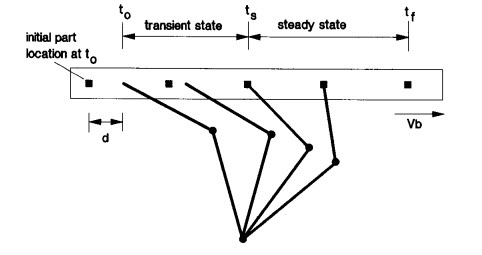
\includegraphics[width=9cm]{Thesis-report/Figures/ik.jpeg}  
    \caption{Kinematics \cite{ref14}}
    \label{fig:Photoneo Cmaera}
\end{figure}

Robot motion must meet certain conditions to maximize the usable performance of the manipulator on conveyor tracks, including \cite{ref14}:
\begin{enumerate}
    \item \textbf{Steady-state error} : The task's accuracy may be reduced due to location and velocity errors in the steady state. Therefore, the steady-state error in the conveyor tracking trajectory must be as low as possible \cite{ref14}.
    \item \textbf{Constraints on torque and smoothness}: The trajectory must be created so that all joint torques remain within their ranges at all times\cite{ref14}.
    \item \textbf{Settling time}The time needed for the task gets less as the robot quickly reaches a steady state.The robot's torque and smoothness restrictions, the conveyor belt speed, and the initial positions of the robot and the part should all be considered for minimizing the settling time\cite{ref14}.
\end{enumerate}
The joint variables in the forward kinematics issue establish the end-effector's position and orientation in Cartesian space, also known as the workspace. The link extensions for prismatic joints and the angles between the links for rotational joints are the joint variables. Finding the values of the joint variables that allow the manipulator to reach the designated location, given a desired end-effector position and orientation, is the challenge of inverse kinematics.  Figure 2 below shows the connection between joint space, Cartesian space, and forward and inverse kinematics\cite{ref10}.\\

\begin{figure}[h]
    \centering
    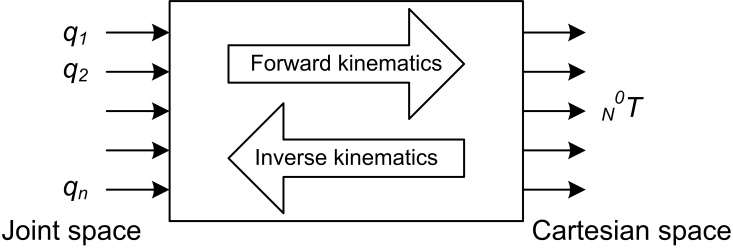
\includegraphics[width=12cm]{Thesis-report/Figures/fk.png}  
    \caption{Forward and Inverse Kinematics \cite{ref10}}
    \label{fig:inverse-kinematics}
\end{figure}

Finding the joint variables that allow a robot to be manipulated into the required position requires an understanding of its inverse kinematics. This is used to control the robot's position, motion, and other features. This study presents a detailed explanation and comparison of two popular approaches for manipulating robots: Jacobian inverse techniques and inverse kinematics.Sixteen alternatives are available for a general six-DOF robot, as shown below, and they list the number of analytical solutions for robots with varying degrees of freedom. Consequently, a precise set of answers among several inverse kinematic solutions is needed for a robot to move constantly\cite{ref10}.\\


The benefit of analytical expression is that it provides formulas for the connection between link parameters and joint angles. The robotics controller can directly incorporate these relationships\cite{ref10}.\\

\begin{table}[h]
    \centering
    \begin{tabular}{cc}
        \toprule
        \textbf{DOF} & \textbf{Number of Solutions} \\
        \midrule
        6 (6R, 5RP) & 8 \\
        6R (intersecting wrist)
Greater than 6 & 16\\
        (Redundant manipulator) & inf.\\
        \bottomrule
    \end{tabular}
    \caption{DOF vs. Number of Solutions \cite{ref19}}
    \label{tab:dof_solutions}
\end{table}
\newpage
\subsection{Jacobian inverse method}
The time derivative of the kinematic equations that connect the end-effector's velocity to the joint rates is known as the Jacobian in robotics. The following is the phrase for the Jacobian \cite{ref19}.
\subsubsection{Kinematic Velocity Equations}

The following equations are taken from \cite{ref19}:
The end-effector angular and linear velocities are given by
\begin{align}
  \omega_e &= J_{\omega}(\theta)\,\dot{\theta}, \\
  v_e      &= J_{v}(\theta)\,\dot{\theta},
\end{align}
where,

\begin{description}
  \item[$\theta$]%
    Joint coordinate vector of size $n$.
    \begin{itemize}
      \item 0i is the i-th joint displacement for prismatic joints, and 0i is the i-th joint angle for revolute joints.
    \end{itemize}

  \item[$\dot{\theta}$]%
    Joint velocity vector (time derivative of $\theta$).
    \[
      \dot{\theta} = \begin{bmatrix}
        \dot{\theta}_1 \\ \dot{\theta}_2 \\ \vdots \\ \dot{\theta}_n
      \end{bmatrix},
    \] 
    with units: rad/s for revolute and m/s for prismatic joints.

  \item[$J(\theta)$]%
    Geometric Jacobian, a $6\times n$ matrix mapping $\dot\theta$ to the end-effector twist.
    \[
      J(\theta) = 
      \begin{bmatrix}
        J_v(\theta) \\[6pt]
        J_\omega(\theta)
      \end{bmatrix}.
    \]

  \item[$J_v(\theta)$]%
    Linear‐velocity submatrix of $J$. It’s the top 3 rows:
    \[
      J_v(\theta) \in \mathbb{R}^{3\times n},
      \quad
      v_e = J_v(\theta)\,\dot\theta
      \;\in\; \mathbb{R}^3.
    \]

  \item[$J_\omega(\theta)$]%
    Angular‐velocity submatrix of $J$. It’s the bottom 3 rows:
    \[
      J_\omega(\theta) \in \mathbb{R}^{3\times n},
      \quad
      \omega_e = J_\omega(\theta)\,\dot\theta
      \;\in\; \mathbb{R}^3.
    \]

  \item[$v_e$] the end‐effector linear velocity vector in the base/world frame:
    \[
      v_e = \begin{bmatrix} \dot{x} \\ \dot{y} \\ \dot{z} \end{bmatrix},
    \]

  \item[$\omega_e$]is the end‐effector angular velocity vector in the base/world frame:
    \[
      \omega_e = \begin{bmatrix} \omega_x \\ \omega_y \\ \omega_z \end{bmatrix},
    \]
\end{description}
where the $3\times6$ matrices $J_\omega$ and $J_v$ relate the joint velocities or rates $\theta$ to the end-effector velocity $v_e$ and angular velocity $\omega_e$, respectively. Note that $J_\omega$ and $J_v$ are both functions of $\theta$, denoting the relation to the robot orientation. It is possible to rewrite the end effector displacement as a function of the Jacobian $J(\theta)$ as \cite{ref19}:

  \[
    \Delta x_e = J(\theta) \, \Delta \theta 
  \]

This is a first-order Taylor expansion and is valid for small $\Delta \theta$
\newpage
\subsection{Inverse Kinematics Using Jacobian}

If the Jacobian $J(\theta)$ is square and invertible (e.g., for a 6-DOF manipulator), then:\cite{ref19}

  \[
    \Delta \theta_k = J_k^{-1} \Delta x_e ,
  \]

And the joint update becomes:

  \[
    \theta_k = \theta_{k-1} + J_k^{-1} \Delta x_e  
  \]

\subsection{Redundant manipulators and pseudoinverse Solution}

For manipulators where $J$ is not square (e.g., redundant robots with $n > 6$), we use the moore–Penrose pseudoinverse $J^\dagger$:\cite{ref19}

  \[
    \theta_k = \theta_{k-1} + J^\dagger \Delta x + (I - J^\dagger J)\Delta \phi 
  \]

where:
\begin{itemize}
    \item $J^\dagger$ is the pseudoinverse of $J$ \cite{ref19}. 
    \item $(I - J^\dagger J)$ projects into the null space of $J$\cite{ref19}.
    \item $\Delta \phi$ is a secondary objective function direction (e.g., for obstacle avoidance or joint limit avoidance)\cite{ref19}.
\end{itemize}

\subsection{Jacobian Construction}

Every column in the Jacobian matrix represents a joint's contribution to the motion of the end-effector: \cite{ref19}.
\begin{itemize}
    \item For a revolute joint $i$:\cite{ref19}.
    \[
        J_i = \begin{bmatrix}
            \mathbf{z}_i \times (\mathbf{o}_n - \mathbf{o}_i)\\
            \mathbf{z}_i 
        \end{bmatrix}
    \]
    \item For a prismatic joint $i$:\cite{ref19}.
    \[
        J_i = \begin{bmatrix} 
            \mathbf{z}_i \\
            \mathbf{0}
        \end{bmatrix}
    \]
\end{itemize}
where:
\begin{itemize}
    \item $\mathbf{z}_i$ is the axis of joint $i$ in base coordinates.
    \item $\mathbf{o}_i$ is the origin of frame $i$, and $\mathbf{o}_n$ is the end-effector origin.
\end{itemize}

\subsection{Robot Coordinate System} 
We must first gain a fundamental understanding of the robot coordinate system before delving deeper into the tracking system's operation. Generally speaking, robotic systems are Cartesian coordinate systems with three axes: the X, Y, and Z axes. Additionally, there is the Rotation Coordinate System, which describes the robot's degree of rotational motion and joint function. However, as this format is more widely used in business and simpler to use and comprehend, we shall solely investigate the Cartesian coordinate system. The following terms used in the system should be understood to obtain the robot's coordinates \cite{ref24}.

\subsubsection{System of World Coordinates (WCS)}
A coordinate system is often specified by the user or developer, but it can exist anywhere in the world. WCS makes it simpler to explain the locations of other things or items in that specific area. Origin placement is typically done at the edge of a group or a room's corner \cite{ref24}.\\

 \textbf{Machine Coordinate System (MCS)}
Robot Base Frame Coordinate System is another name for machine Coordinate System (MCS). All other coordinate systems will be compared to this most significant coordinate system. Where developers and programmers would implement their code based on this coordinate system is equally crucial. For the point of origin, mCS is usually placed close to the robot's base, though it's crucial to keep in mind that different robot types have different bases \cite{ref24}.\\

 \textbf{Coordinate System for parts and Workpieces (PCS)}
The workpiece or monitored items that move along the conveyor belt are referred to here. In certain applications, part orientation plays a crucial role in assembly procedures. In our application, we just want to choose or select the objects, independent of their orientation; thus, this isn't accurate\cite{ref24}.\\

 \textbf{Tool Coordinate System (TCS)}
 This refers to the location of the robot's end-tip. As you can see, a robotic hand typically has a mechanism attached to the end with a gripper. When referring to the robot base frame, this typically requires a small amount of offset and aids the robot in completing its responsibilities \cite{ref24}.
 \textbf{ Coordinate Transformation matrix}  \\
 In essence, the coordinate transformation matrix is a matrix that depicts how a coordinate system's orientation changes from one frame to another. It describes both rotation and translation transformation and is composed of a 3x3 rotation matrix and a 3x1 displacement vector.  In the case of three dimensions, the matrix is 4x4.  The homogeneous transformation matrix is a more popular and often used term for this matrix.  Keep in mind that this matrix can be used for forward kinematics calculations and standard coordinate transformation procedures, among other coordinate transformation scenarios \cite{ref24}.

\begin{figure}[h]
    \centering
    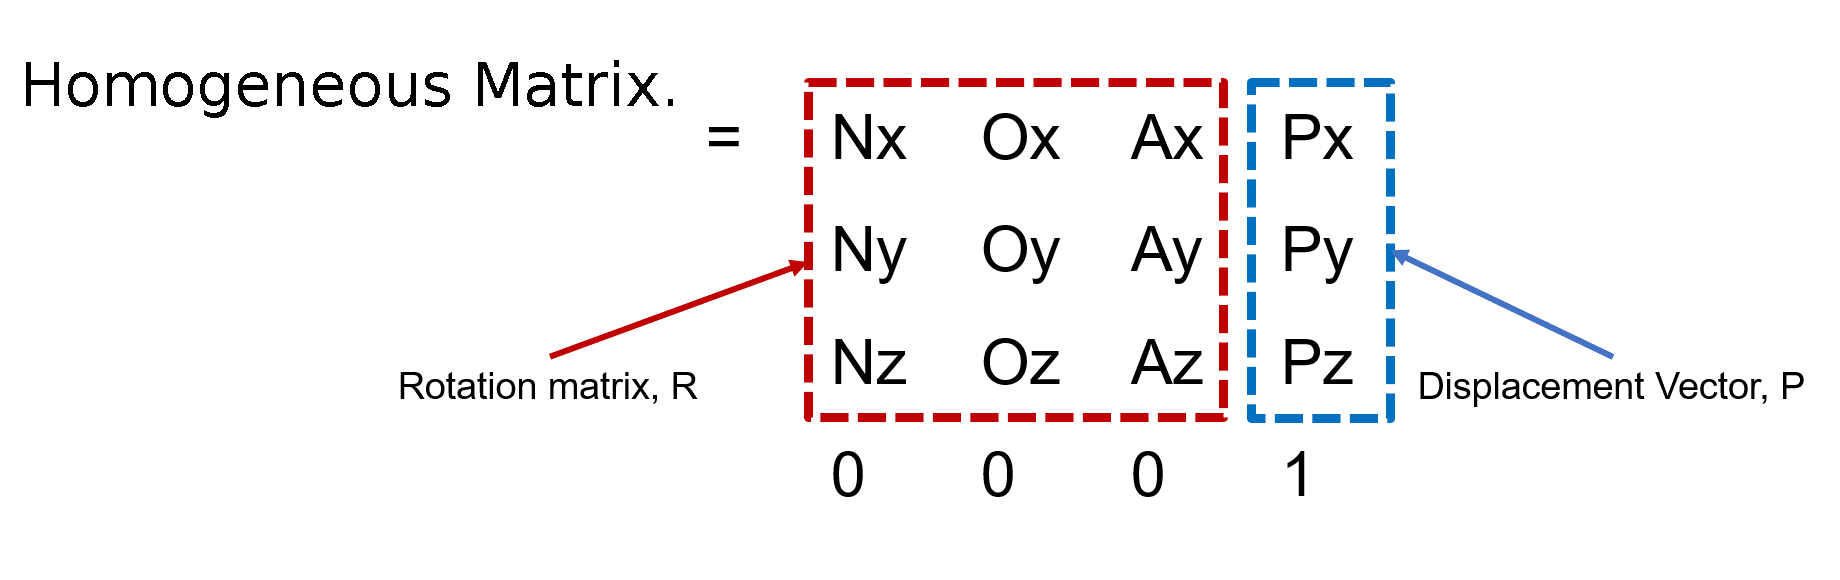
\includegraphics[width=15cm]{Thesis-report/Figures/transform.png} 
    \caption{Homogenous transform \cite{ref25}}
    \label{fig:Photoneo_Camera}
\end{figure}
\newpage
\section{Working Principle}
\subsection{Workflow}
\begin{enumerate}
    \item Start
    \item Initially, check if the operation type is OBJECT pOSE
    \item If not, raise a problem to demonstrate that there is an unforeseen problem.
    \item If yes: Receive object pose data
    \item Then unpack the object pose and set them as ([X,Y,Z,ex,ey,ez])
    \item Convert the first three elements to meters ([X.Y, Z])
    \item Set the velocity and timeout for picking
    \item Record the start time
    \item Calculate the current time and update the position X with the equation \[  
X = X_0 + v\,t
\]

    \item Create the target position with the quaternion values received from the camera
    \item Check the condition where the object needs to be picked; if the distance is less than 700, then do the motion of move linear ()
    \item If not successful,  break the loop and print that the target is too far
    \item Get the current joint angles and TCP pose, and calculate the distance to the object.
    \item If the distance to the object is less than 5, then send the signal to the gripper and pick the object.
    \item If the timeout to pick is greater compared to the given input, then break the loop.
\end{enumerate}
\newpage
The following figure shows the flowchart for the dynamic picking:\\
\begin{figure}[h]
    \centering
    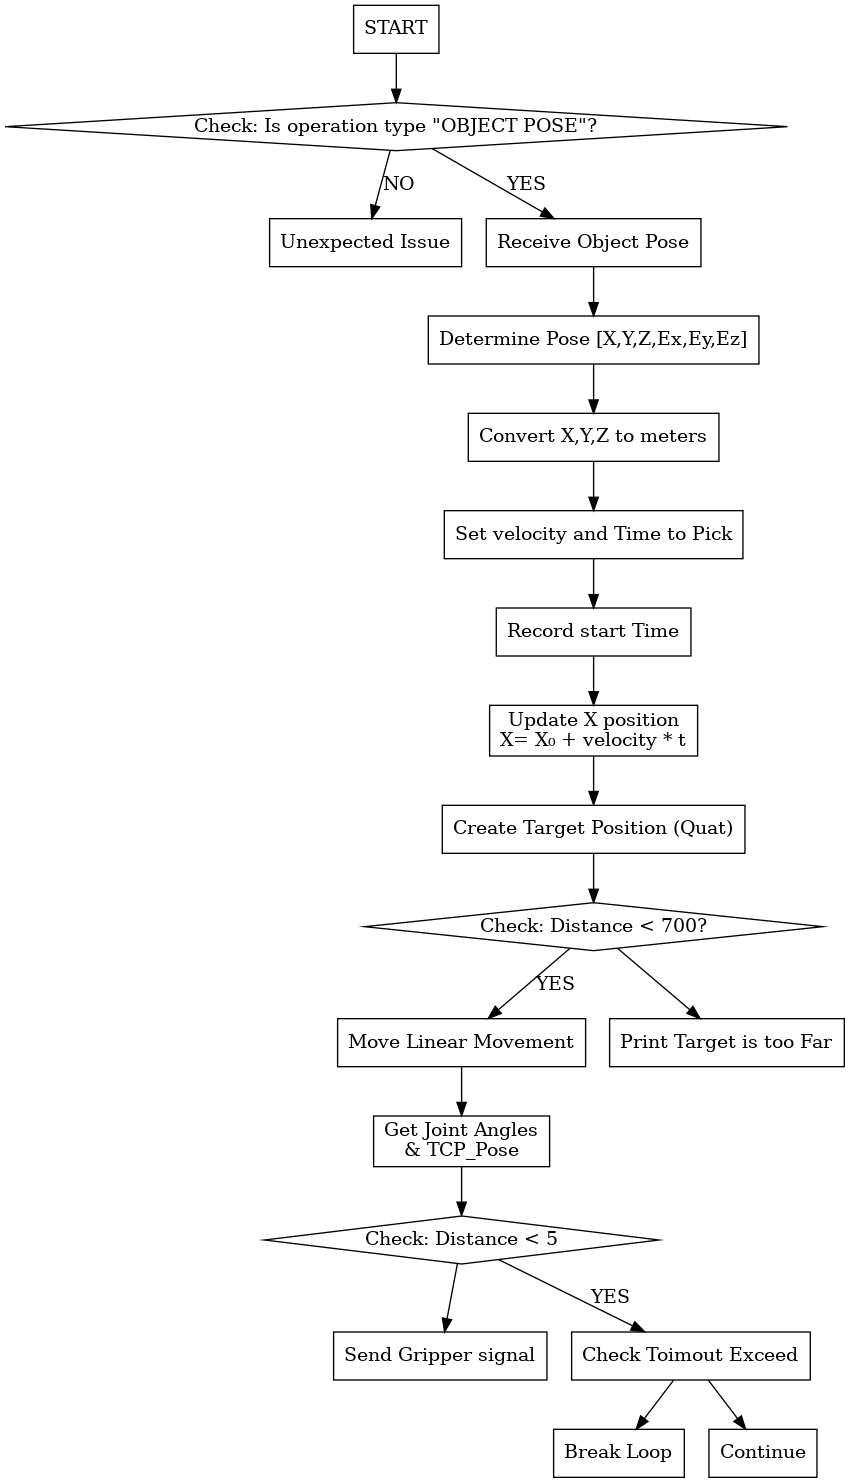
\includegraphics[width=10.3cm]{Thesis-report/Figures/flowchart.png}  
    \caption{Working principle flowchart}
    \label{fig:working-principle}
\end{figure}
\newpage

\newpage

\subsection{Pillars of the Tracking System}
The tracking system's pillars are composed of three primary components. Only a scenario including a camera, a belt conveyor, and a robot will be covered in this post. It is certainly possible to expand the tracking system by including additional robots and cameras. The principles will not change, even if more complex processes will be needed to account for extra elements\cite{ref25}.\\

\subsubsection{Conveyor Belt to Camera Conversion (B1)}
The orientation of the conveyor belt coordinates and the camera origin coordinates deviate from one another. The origin of a camera is the upper left corner of its field of vision (FOV), where the values of its pixels start at (0, 0). This origin is set in stone and cannot be altered. Although the origin's location for the conveyor belt can be freely specified, the normal practice is to first select the picking window's dimensions (it is square), taking into account the robot's picking range limit, and then position the origin in the middle of the bottom of the window\cite{ref25}.\\

\begin{figure}[h]
    \centering
    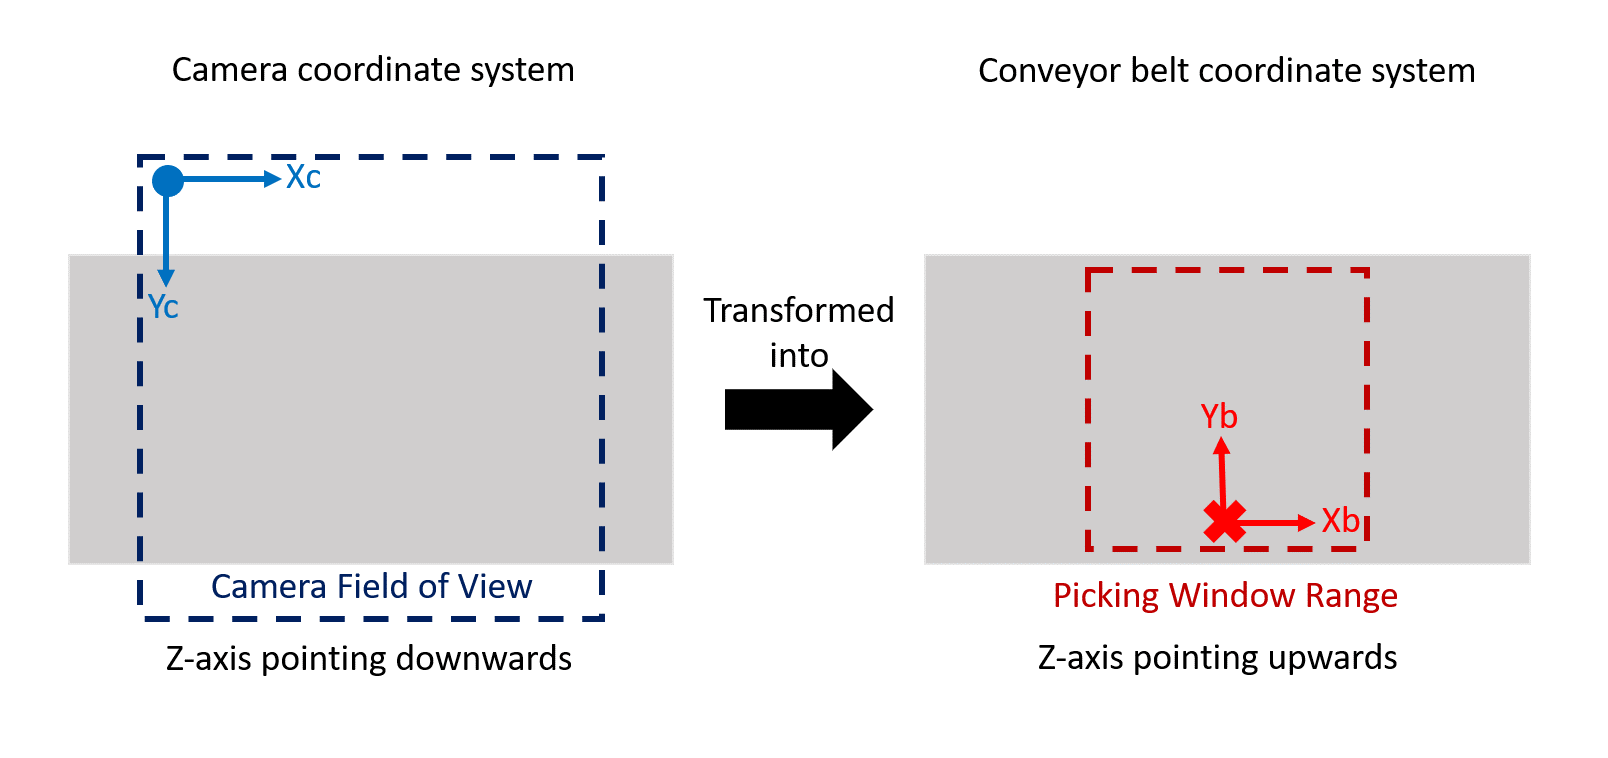
\includegraphics[width=15cm]{Thesis-report/Figures/camera to conveyor.png}
    \caption{Conveyor to camera conversion \cite{ref25}}
    \label{fig:conveyor}
\end{figure}
As can be seen in the above image, to match the origin of the conveyor belt, we must perform a translation transformation on both the X and the Y axes. We must do a rotation transformation for the Z-axis, since the belt origin faces the other direction from the camera origin. In summary, this section contains two transformations: the rotation transformation, $\text{Rot}(x, 180^\circ)$, and a translation in the X-axis and Y-axis, $\text{Trans}(\Delta X, \Delta Y, 0)$. Observe that both the Y and Z axes changed their facing directions when we rotated the X axis. For this section, some offset will be required \cite {ref25}.\\

\subsubsection{Conveyor belt (B1) to conveyor belt (B2) transformation}
For this part, it is quite simple. This transformation is about the movement of the conveyor belt from the camera’s field of view to the robot’s workspace/pick range. The only value that changes in this transformation is the X-axis value. As was indicated in the beginning, we also use the encoder's reading to monitor the conveyor belt's travel distance\cite{ref25}.\\

\begin{figure}[h]
    \centering
    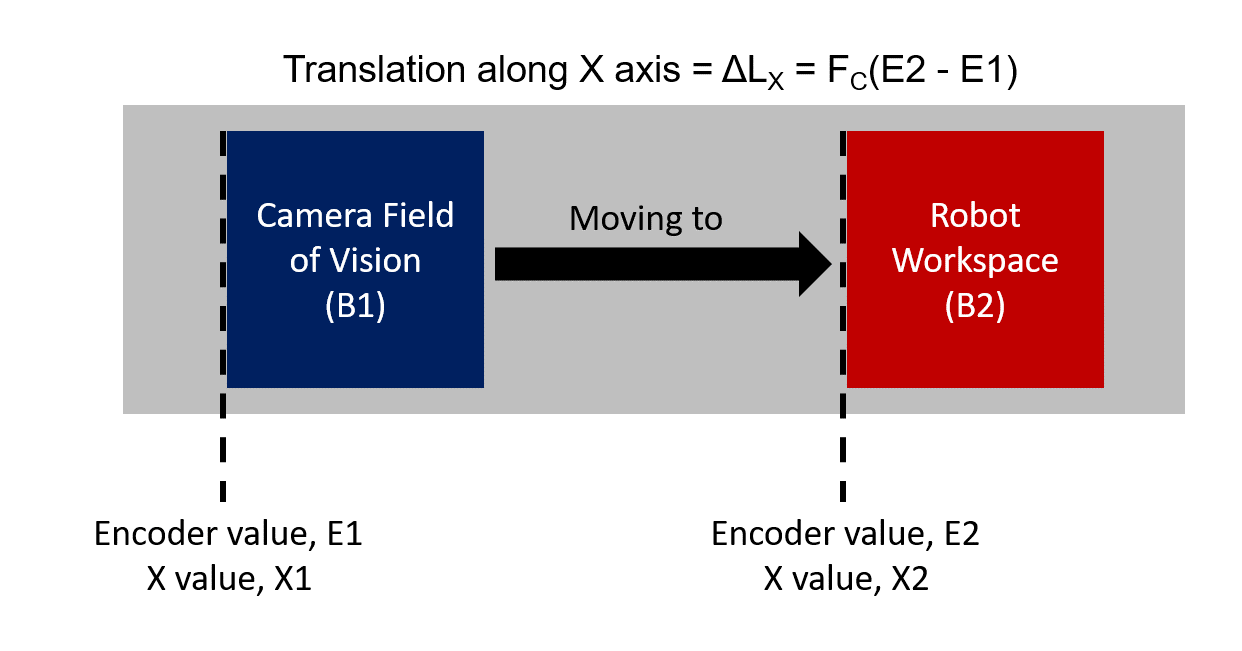
\includegraphics[width=10cm]{Thesis-report/Figures/cam to conv.png}
    \caption{Conveyor belt b1 to b2 conversion \cite{ref25}}
    \label{fig:conv-b12}
\end{figure}
\newpage
\subsection{Robot Motion Modes}
The robot can be operated with 3 motion modes, namely \textit{ServoX}, \textit{ServoJ}, and \textit{MoveLinear}.\

\begin{enumerate}
    \item \textbf{ServoX.} The Servo X motion involves moving the robot in Cartesian motion, using the quaternion poses $[X, Y, Z, Q_x, Q_y, Q_z, Q_w]$ as a representation of the coordinates we receive from the camera.These are already in Cartesian poses, which can be directly passed to the robotic controller, giving these values as the target position and moving the robot to the desired location. During motion, the camera coordinates were not in the correct order as those of the robotic movement, so initially, the target position had to be changed as in this form [X, Y, Z, W, Qx, Qy, Qz].
    \item \textbf{ServoJ.} When using ServoJ, the robot moves with the joint movements rather than Cartesian. The object coordinates that we get from the camera are in Cartesian form; they need to be converted into joint form and given as the target position. The final orientation values of the coordinates when providing the target position will differ from the robot's TCP coordinates. To set this, we have to implement the method of inverse kinematics.
    \item \textbf{MoveLinear.} With the movelinear controller, the camera scans the objects to deliver the quaternion values, which are then used to immediately determine the target position for the robot to pick up the object. Here, we specify the top speed and acceleration.  Through a servo interface, quaternion values are sent to the robot as the target position in order to move it to the desired location.
\end{enumerate}

\newpage
\subsection{Coordinate Transformation}
The availability of 3D data is essential for numerous applications in the fields of vehicle automation ,manufacturing and autonomy.  Time-of-flight (ToF) sensors are getting cheaper and more available. They offer in-depth information for every pixel at every pixel in addition to intensity. Within its field of vision, the ToF sensor gives spherically coordinated range data about the surrounding environment. The spherical coordinates are transformed into Cartesian coordinates, as described in the following section, with the origin of the coordinate system located at the center of the camera.  With the origin at a known reference point, the 3D point cloud in the camera coordinate system is converted to the belt coordinate system. The tests examine the capacity of ToFsensors to provide sensing for a robot tasked with handling goods traveling on a conveyor belt in an indoor scenario. The range data is utilized to identify and calculate the dimensions of objects traveling along a conveyor belt.  The robot then receives the geometry and recognition data for additional action.  The findings suggest that ToFsensors have immediate potential for automating these kinds of applications \cite{ref5}.\\

 The coordinate transformation is necessary for two reasons:\cite{ref5}
 \begin{enumerate}
     \item  To enable the robot to be guided by the range camera's measurements, the robot and the camera must agree on a coordinate system\cite{ref5}.

    \item In the belt coordinate system, the z-axis is normal to the belt plane.  By referring to points above the belt plane ($z >= 0$) and inside the belt limits, this alignment of the coordinate axis makes it easier to extract item point clouds on the belt \cite{ref5}.
 \end{enumerate}
 \subsection{Robotic motion}
Given a point in the world coordinate, the angle of each joint is calculated based on an inverse kinematics (IK) equation. In general, there may be no analytic IK solution from a manipulator for the configurations of each joint. The numerical method is introduced to solve the problem for
general manipulators. The velocity of the joint can be mapped to Cartesian space with the Jacobian linearization method\cite{ref19}.
\\

\[
v = J(q) \dot{q} 
\]

Pseudo-inverse is used to solve the joint:\cite{ref19}


\[
\dot{q} = J^\dagger \dot{x}, \quad J^\dagger = (J^T J)^{-1} J^T
\]

Velocity for the linear velocity in Cartesian space. First, FK is used to determine the manipulator's pose. Next, the IK solver uses a pseudo-inverse calculation to update the joint angles. Until the end tip reaches the desired posture with an acceptable error, these two stages are repeated. If the starting value and changing rate are appropriately calibrated, the dynamic gain causes the speed to reach its maximum and minimum quickly. Joint angles have an impact on the inaccuracy during the iteration process. Inappropriate angles cause the gain to drop dynamically, and vice versa \cite{ref19}.

\subsubsection{Steps for Conveyor Tracking Visual System}

Two steps are necessary for conveyor visual tracking: \cite{ref12}
\begin{itemize}
\item Item detection
\item Object tracking.
\end{itemize}
There are several ways to identify items. Some potential limitations are, however,info-based recognition, self-organizing maps, template matching, and the temporal difference between two consecutive image samples. Due to their slowness, self-organizing maps cannot function in real time. To match objects, template matching necessitates prior object information knowledge.  Unfortunately, this approach cannot be employed in real time due to the required processing load. The color information solution overcomes the first two limitations; however, it is not compatible with binary images. The object recognition method that leverages the difference between two photographs can be useful when the environment does not change quickly over time\cite{ref12}.
\subsubsection{Photoneo Camera}
The main Vision camera we have used to track the moving object's motion through the conveyor belt is a photoneo camera (MotionCam 3D m+), which has advanced settings that can capture and detect the object's position.The photoneo camera mainly consists of 3D sensing technology, which contains parallel structured light that helps provide the light source to detect objects. This camera is capable of capturing conventional intensity images of the object as well as precise point clouds.[2]. Three parts comprise the 3D camera: a camera unit with our proprietary mosaic Shutter CMOS image sensor, a laser projection unit, and a processor unit with a GPU that acts as the brain behind intelligent applications. A sequential structured light, which is utilized in numerous meteorological applications, is the primary technological driver in the first group. One well-suited representative of this category is the 3D scanner range from photoneo \cite{ref2}. \

\subsubsection{Robot Interface}
There are two software components, which include
\begin{enumerate}
    \item   Robot interface: utilized to configure the vision controller's Ethernet port on the network\cite{ref2}.
    \item   Robot controller: utilized to determine the robot controller's IP address\cite{ref2}.
\end{enumerate}
\begin{figure}[h]
    \centering
    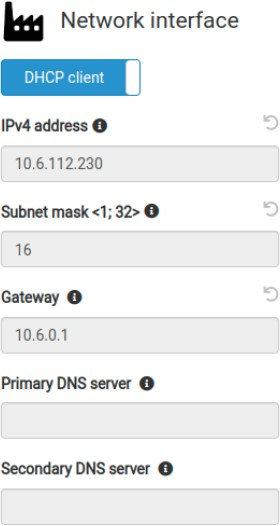
\includegraphics[width=5cm]{Thesis-report/Figures/network_interface.jpeg}
    \caption{Robot Network Interface\cite{ref2}}
    \label{fig:network-interface}
\end{figure}
 As outlined in the Robot Communication, the Action Request Communication Channel helps the visual controller and the robotic controller communicate with one another.  The vision controller creates a TCP server, which the robotic controller connects to and sends requests to.
 It is advised to keep the Action Request Server port section empty and use the default port for this TCP server.  It is necessary to use the same port on the robot side when a custom port is defined \cite{ref2}.

\subsubsection{Vision Controller Interface}
To connect the 3D sensor, gigabit Ethernet cables (Cat5e or higher category) are required.  multiple 3D sensors can be connected using a gigabit switch.  The switch or Ethernet connection of the 3D sensor is always connected to the network of the scanner \cite{ref2}.
\begin{figure}[h]
    \centering
    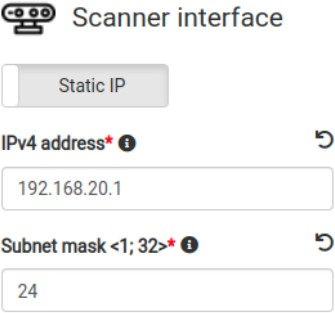
\includegraphics[width=5cm]{Thesis-report/Figures/scanner_interface.jpeg}
    \caption{Robot Network Interface \cite{ref2}}
    \label{fig:scanner-interface}
\end{figure}

 Setting up localization settings, calibrating the robot camera, and seeing 3D scans all require a well-configured connection to the 3DSensor. To set up the network interface that the vision controller uses to connect to the photoneo 3D Sensor, select the Scanner Interface section under the Network tab\cite{ref2}.\\

 photoneo 3D Sensors have both a programmable IPv4 address and a fixed IPv6 link-local address. IPv6 connections are better than IPv4 ones. However, in the event that the IPv6 connection is blocked or fails, the IPv4 address is used.  It is therefore recommended to have a valid IPv4 network configuration. We use the proper IP address settings on the sensor side using the phoXi Control program in all scenarios. The interface can be configured to run a DHCP server or to use any random static IP address\cite{ref2}.\\

\subsubsection{Communication of Robot With Vision Camera}
Communication between the vision controller and the robot controller is made possible via the robot interface on the vision controller and the robot module running on the robot controller\cite{ref2}.\\

\begin{figure}[h]
    \centering
    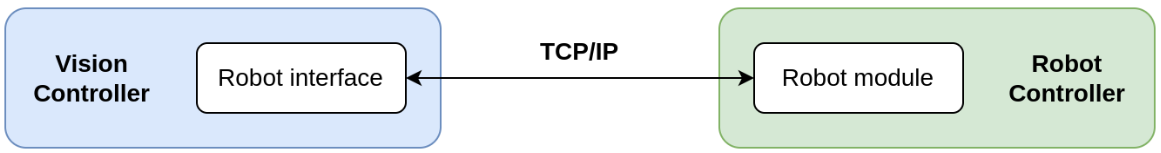
\includegraphics[width=14cm]{Thesis-report/Figures/communication.png}
    \caption{Communication with camera \cite{ref2}}
    \label{fig:camera-comms}
\end{figure}

The Vision Controller's scanner port is directly attached to a single photoneo 3D sensor. 
The vision controller's network port is directly connected to a desktop pC for remote control.
The robot controller is directly attached to the vision controller's robot port\cite{ref2}.

\begin{figure}[h]
    \centering
    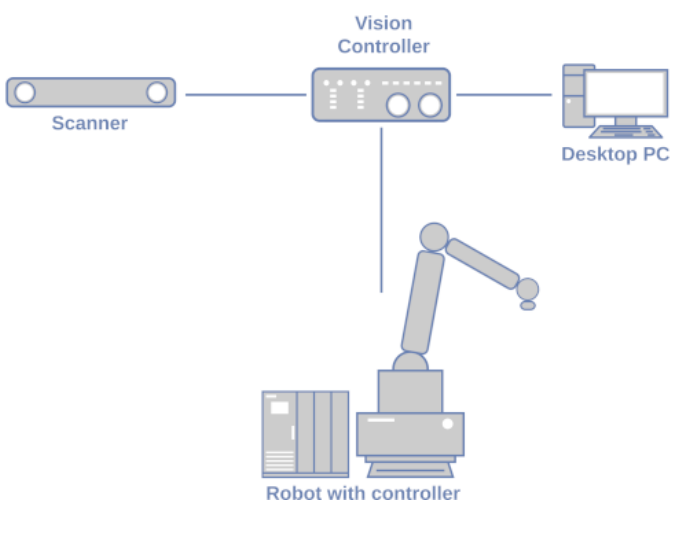
\includegraphics[width=12cm]{Thesis-report/Figures/connection.png}
    \caption{Whole camera with Robotic controller setup\cite{ref2}}
    \label{fig:whole-camera}
\end{figure}

\newpage
 \subsubsection{Protocol TCP/IP}
The robot controller and the vision controller communicate via the TCP/IP protocol. Network connectivity is an optional feature that some robot controllers do not come with by default\cite{ref2}.

\subsubsection{Channel of communication}
The robot module functions as a TCP client, while the vision controller establishes a TCP server. The client is called the Action Request Client, while the server is called the Action Request Server. The Action Request Client communicates with the Action Request Server over this channel. After receiving the action request, the vision controller carries it out and replies to the robotic controller\cite{ref2}.


\begin{figure}[h]
    \centering
    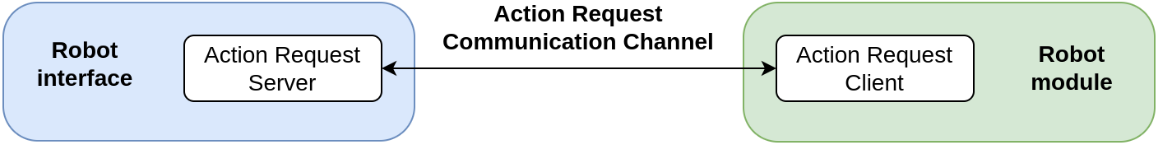
\includegraphics[width=14cm]{Thesis-report/Figures/channel.png}
    \caption{Channel Communication \cite{ref2}}
    \label{fig:Photoneo Camera}
\end{figure}

The robot connection status is currently indicated by the following indicator:

 Action Request Client: The condition of the Action Request Server and the Action Request Client's connection via the Action Request Communication Channel. It may exist in one of two states: \cite{ref2}
 \begin{enumerate}
     \item  \textbf{CONNECTED} Due to its connection to the Action Request Server, the Action Request Client can send requests\cite{ref2}.
      \item   \textbf{DISCONNECTED} The Action Request Client is awaiting a fresh connection because it is not currently linked to the Action Request Server\cite{ref2}.

 \end{enumerate}

 Every vision system has a status indication that shows the current status of the connection to the related photoneo 3D Sensor.

        Each indicator bears the identification number of the vision system to which it belongs.
  \begin{enumerate}
  \item  \textbf{CONNECTED} The vision system's 3D sensor is connected\cite{ref2}.
  \item   \textbf{DISCONNECTED}  There is no connection to the 3D sensor linked to vision system 2\cite{ref2}.
 \end{enumerate}

\subsubsection{Network (EC, HC)}
For the vision controller to connect with the robot and the 3D sensor, the robot interface (and robot controller IP) and the vision controller's 3D sensor interface need to be set up correctly. This is not required for marker space calibration\cite{ref2}.
\subsubsection{Vision }
It is necessary to thoroughly configure the visual system that will be calibrated. make sure the following vision system parameters are set up correctly before beginning the calibration:
 Scanner ID: This vision system uses a 3D sensor. If the scanner interface is configured correctly, the linked 3D sensors will show up in the drop-down list of accessible 3D sensors.
The calibration space and scanner position specify the 3D sensor's mount point and, consequently, the calibration type. The scanner model is automatically calculated based on the selected 3D sensor\cite{ref2}.



%%%%%%%%%%%%%%%%%%%%%%%%%%%%%%%%%%%%%%%%%%%%%%%%%%%%%%%%%%%%%%%%%%%%%%%%%%%%%%%%%%%%%%
\subsubsection{6-Axis Cobot-Delta}
The cobot that we have used for the conveyor tracking system is a 6-axis cobot called a Delta robot. The robot mainly moves towards its target position by getting the values from the camera in the form of quaternion values\cite{ref2}.

\begin{figure}[H]
  \centering
  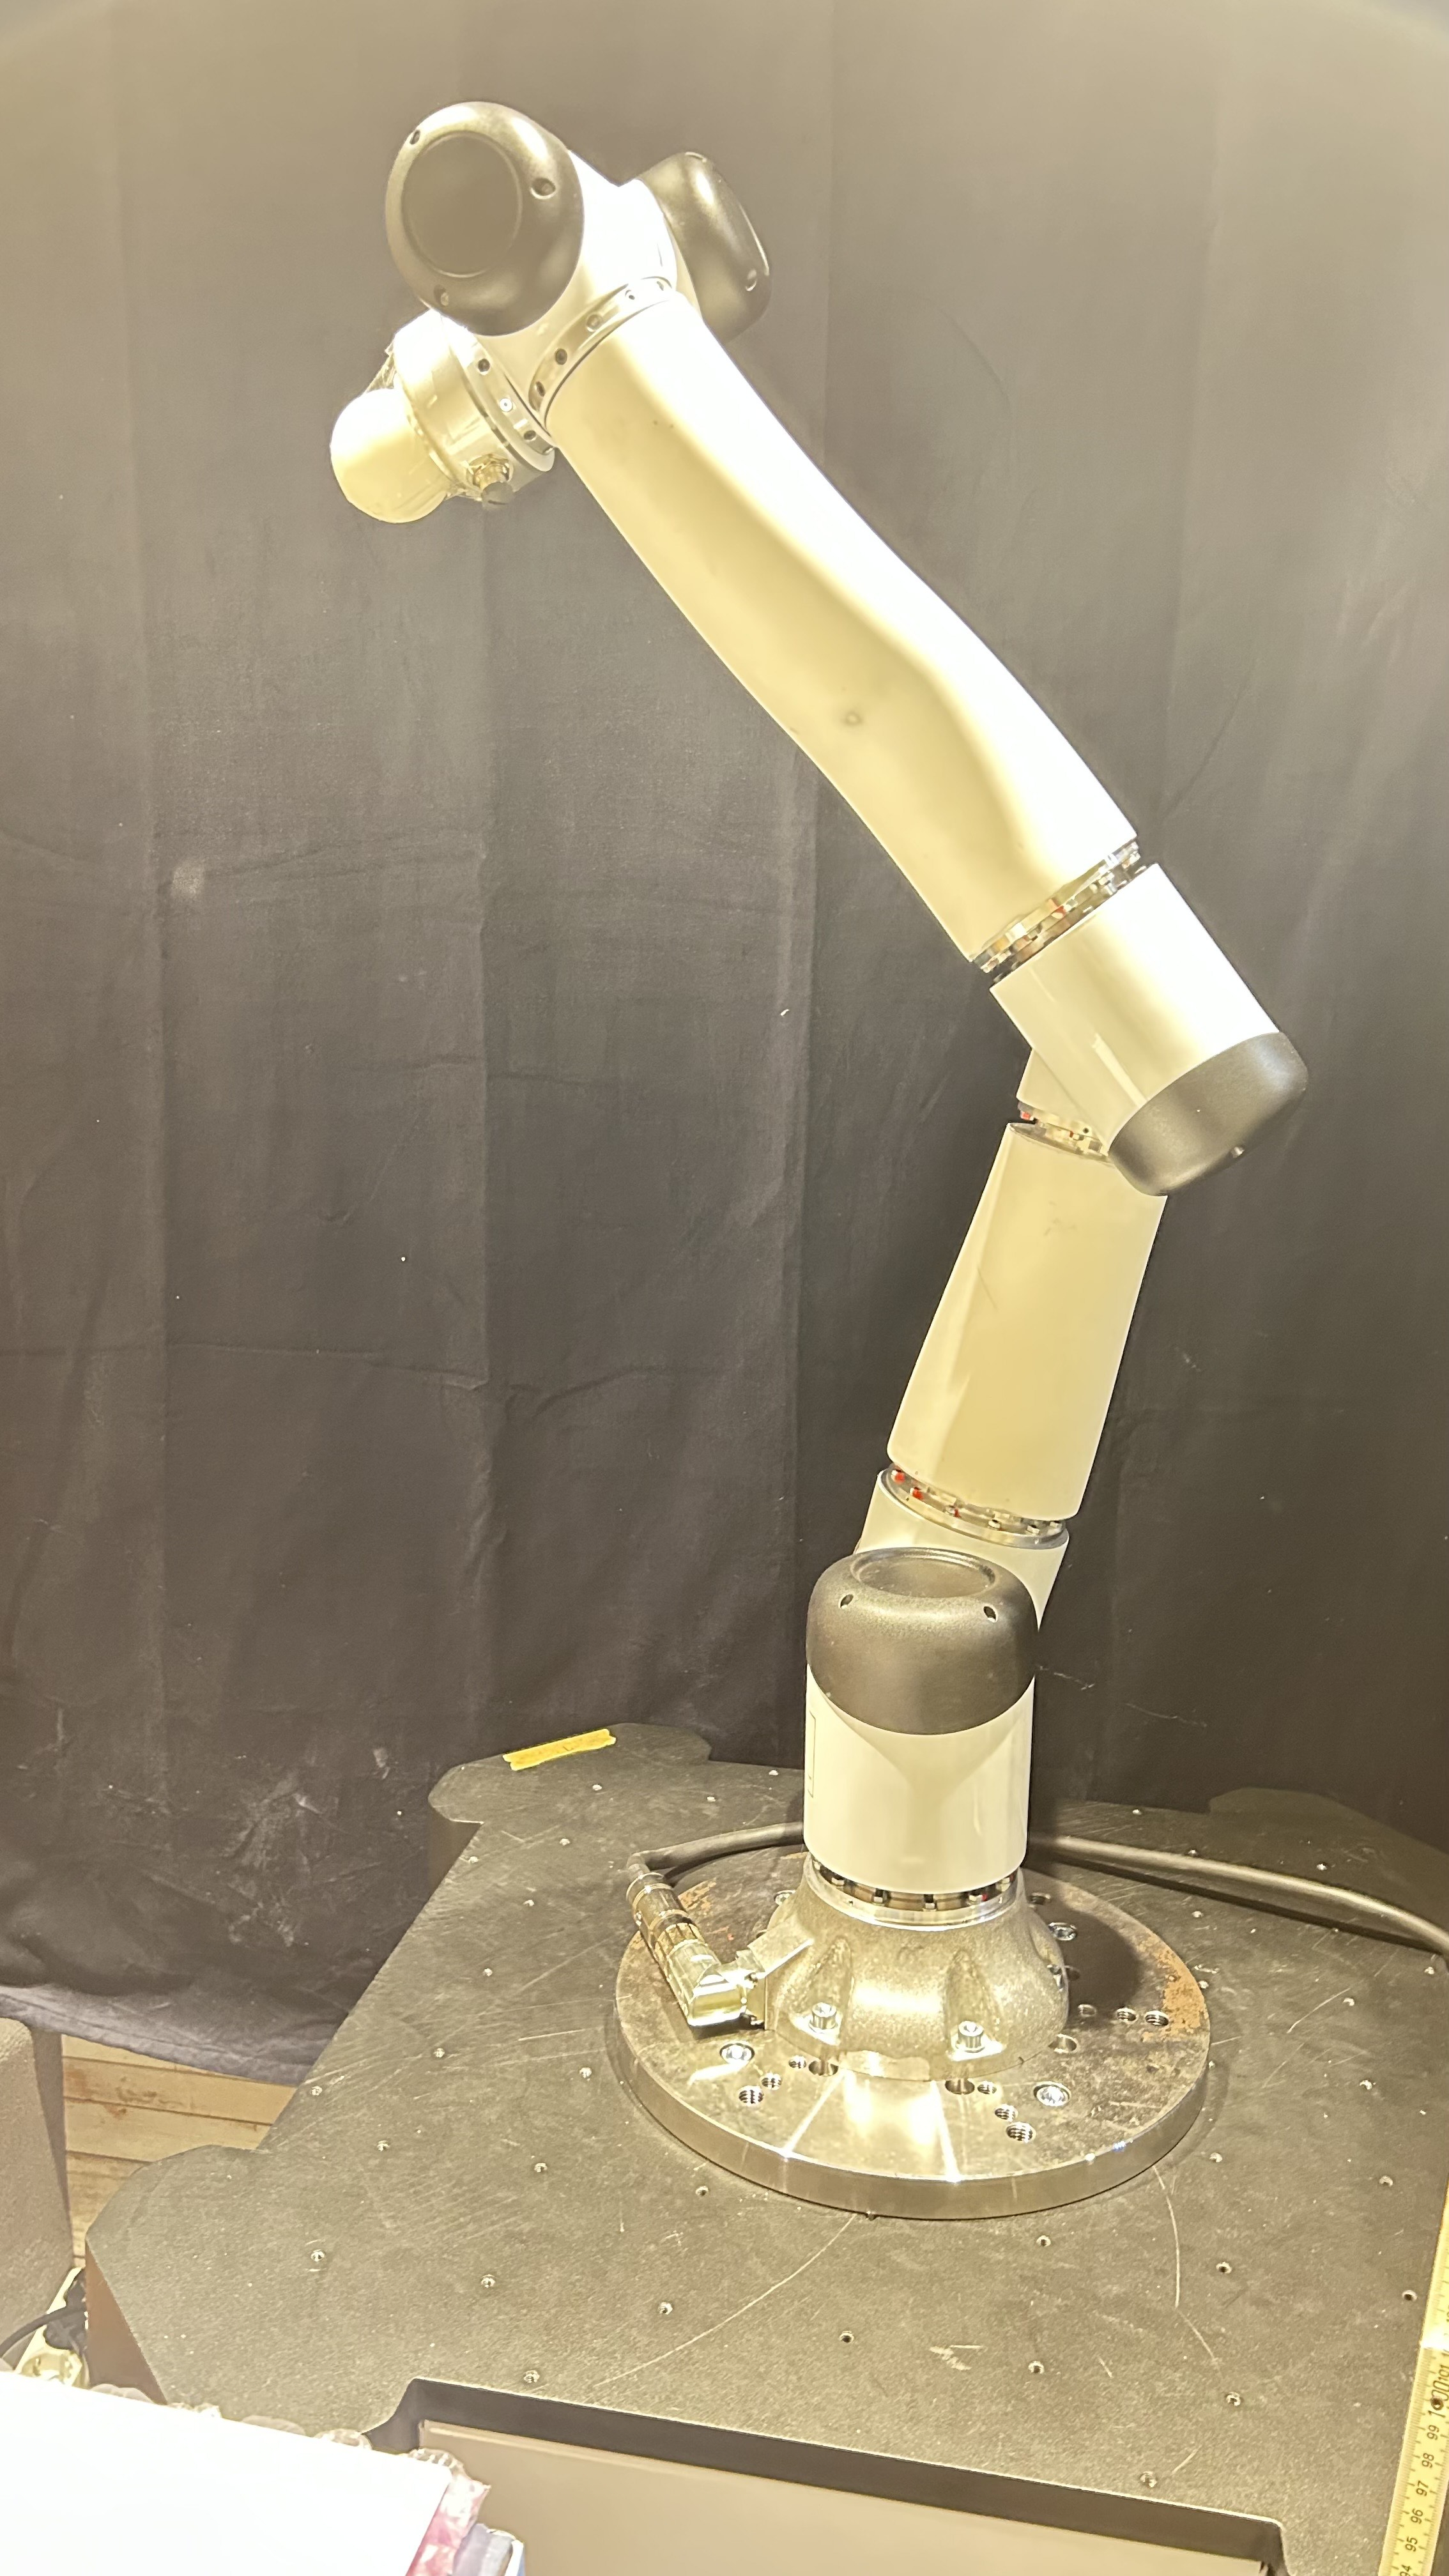
\includegraphics[width=3.5cm]{Thesis-report/Figures/robot.jpeg}
  \caption{Delta Robot}
  \label{fig:delta_robot}
\end{figure}


\subsubsection{RobotiQ 140 Gripper}
The RobotiQ 140 gripper is a two-finger gripper that mainly works under the principle of modbus communication. Its 85 mm stroke, 230 N max gripping force, and 5 kg max payload make it ideal for low-volume, high-changeover settings.

\begin{figure}[H]
  \centering
  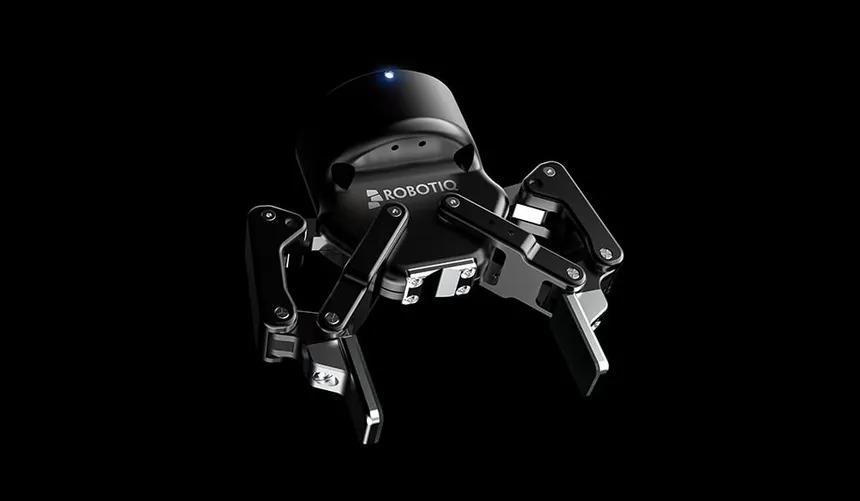
\includegraphics[width=7cm]{Thesis-report/Figures/cobot_gripper_2F_85-ezgif.com-webp-to-jpg-converter.jpg}
  \caption{RobotiQ 140 Gripper\cite{ref26}}
  \label{fig:robotiq_140}
\end{figure}

\subsection{3D Scanning}
The act of gathering data from an object's surface and turning it into data points is known as 3D scanning. These data points are utilized for a digital replication of the scanned object or for a dimension analysis\cite{ref17}.\\

\subsection{Types of 3D scanning}

\subsubsection {Laser Scanning}
Two devices are often used in laser scanning; one directs a laser beam onto a surface, and the other records the precise spot where the object contacts the beam. The angle of reflection and the distance between the surface and the scanner can be determined via triangulation.  Time of flight measurement, structured light scanning, stereophoto-grammetry, laser interferometry, and many other techniques are comparable to the Train-gulation method\cite{ref17}.

\subsubsection {Structure Light Scanning}
This technology projects structured light patterns, such as simple geometric patterns or parallel lines, onto a surface.  The object's shape will cause the patterns to distort.  It is feasible to rebuild the scanned surface using a camera to analyze these deformations, distinguish edges, and determine the separation between the item and the scanner \cite{ref17}.

\subsection {Photogrammetry}
Triangulation is used in photogrammetry to intersect particular points within 2D images based on the angles at which those points can be found. The size, quantity, and quality of the item's images all have a big impact on creating an appropriate 3D model\cite{ref17}. 

\subsection{Time of Flight}
The time of flight is a measure of how long it takes light to move from an illumination source to a scene and back. The main barrier in this case is the speed of light itself.  Time is typically measured using a modulated signal's phase shift. High pixel modulation frequencies must be used to achieve a respectable level of depth accuracy. The primary drawback in this case is physics, since a greater frequency results in less charge transfer, which lowers contrast and Signal‑to‑Noise Ratio. The restriction suggests an accuracy level that ToFsystems can achieve. Usually, it falls within the centimeter range. Another issue is interreflections, which can significantly bend the surface\cite{ref15}.

\subsection{Active stereo}
By projecting a synthetic texture onto an object, active stereo addresses the unreliable passive stereo. Nevertheless, it still has to resolve the computationally demanding picture correspondence matching problem. Because of the complexity of the matching problem, the projected texture can be either high frequency, which can satisfy a higher resolution but usually has poor reliability, or low frequency, which typically uses random laser dots and can provide higher reliability but poor resolution (the features 15 are sparse)\cite{ref15}.

\subsection{Structured patterns/dots}
A spatially encoded pattern is used in structured patterns/dots technology to encode depth disparity information into pattern patches, which are usually projected through a laser diffraction grating in the form of a carefully planned dot collection. The camera needs to be able to see enough of the patch in order to properly record the depth information and reconstruct the code. This produces artifacts on the surfaces' edges and tiny objects. To reconstitute individual dots in the projection (and hence 3D measurements), the Nyquist-Shannon theorem necessitates an order of magnitude better camera resolution. modern systems use about 25 camera pixels for each 3D measurement, producing about 70k 3D points \cite{ref15}. 

\subsection{Parallel Structured Light}

Parallel Structured Light parallelizes the sequential structured light using a sophisticated sensor design, which enables it to record the scene illuminated by various patterns. In addition to sharing many of the sequential structured light's benefits, such as resolution and accuracy, it also overcomes one of its main drawbacks: the inability to capture a dynamic environment. photoneo's parallel Structured Light gets around the restriction by projecting and capturing numerous encoded patterns. pixel modulations within our proprietary CMOS sensor are used to accomplish this. multiple groups of separately modified pixels make up the sensor itself \cite{ref15}.  \\


The parallel Structured Light's main advantages are:
\begin{enumerate}
 \item  Rapid motion scanning: 40 m/s motion is achieved with single frame acquisition \cite{ref15}.
\item A more effective depth coding method with accurate, per-pixel measurement that offers ten times greater resolution and accuracy than rival technologies\cite{ref15}
 \item No motion blur: exposure time of 10 µs per pixel\cite{ref15}
 \item Quick capture of 1068 x 800 point clouds at 60 frames per second\cite{ref15}
\item patent-pending active ambient light rejection technology for outdoor use in direct sunlight\cite{ref15}
 \item Active rejection of ambient light through interreflection suppression\cite{ref15}
\item Several devices using the same space at the same time\cite{ref15}\\
\end{enumerate}

A control unit that operates in tandem with the projection is in charge of these groups. The coded patterns are inserted into the groups rather than changing the projection itself. The coded patterns injected at the end of the frame may cause the sensor to produce more than 20 different virtual representations of the scene.  Any pattern commonly used for sequential structured light can be utilized to adapt the universal approach on the fly to suit different materials and light sources\cite{ref15}. \\

After undergoing embedded processing, these virtual images are sent via gigabit Ethernet to a client pC.  Three types of outputs are provided by the sensor: \cite{ref15}
\begin{enumerate}
    \item point Cloud: 32 bits per channel  XYZ \cite{ref15}
    \item 32 bits per channel is the normal map.  XYZ \cite{ref15}
    \item Texture: Grayscale, 10/12 bits \cite{ref15}
\end{enumerate}

The sensor produces outputs with a resolution of 1068 x 800 when in "one frame" camera mode.  Approximately 500k individual measurements were used to interpolate these positions. The typical z-noise standard deviation at a distance of one meter is less than 0.5 mm (key advantage 1).  Because of the pixel design, each photon makes the best possible contribution to the 3D measurement.  The technology surpasses its rivals and offers the best XYZ resolution thanks to sub-pixel accuracy coding (high z-precision) and an efficiency of just 4.5 pixels per 3D measurement (benefit 2)\cite{ref15}. \\

The "scanner mode," which is designed for still photos, is the alternate operating mode.
 The sensor's raw sensoric output in this mode is 1602 × 1200 individual measurements. This is recorded in three consecutive frames. A laser that has been deflected by a mirror illuminates the scene.  The projection's 10 µs per pixel exposure may guarantee constant, motion-blur-free data (benefit 4)\cite{ref15}.


\subsection{Vision Controller}
The figure 3 below shows the vision controller connected to the photoneo camera and the robotic controller using Ethernet (IPV4 address).
\begin{figure}[h]
    \centering
    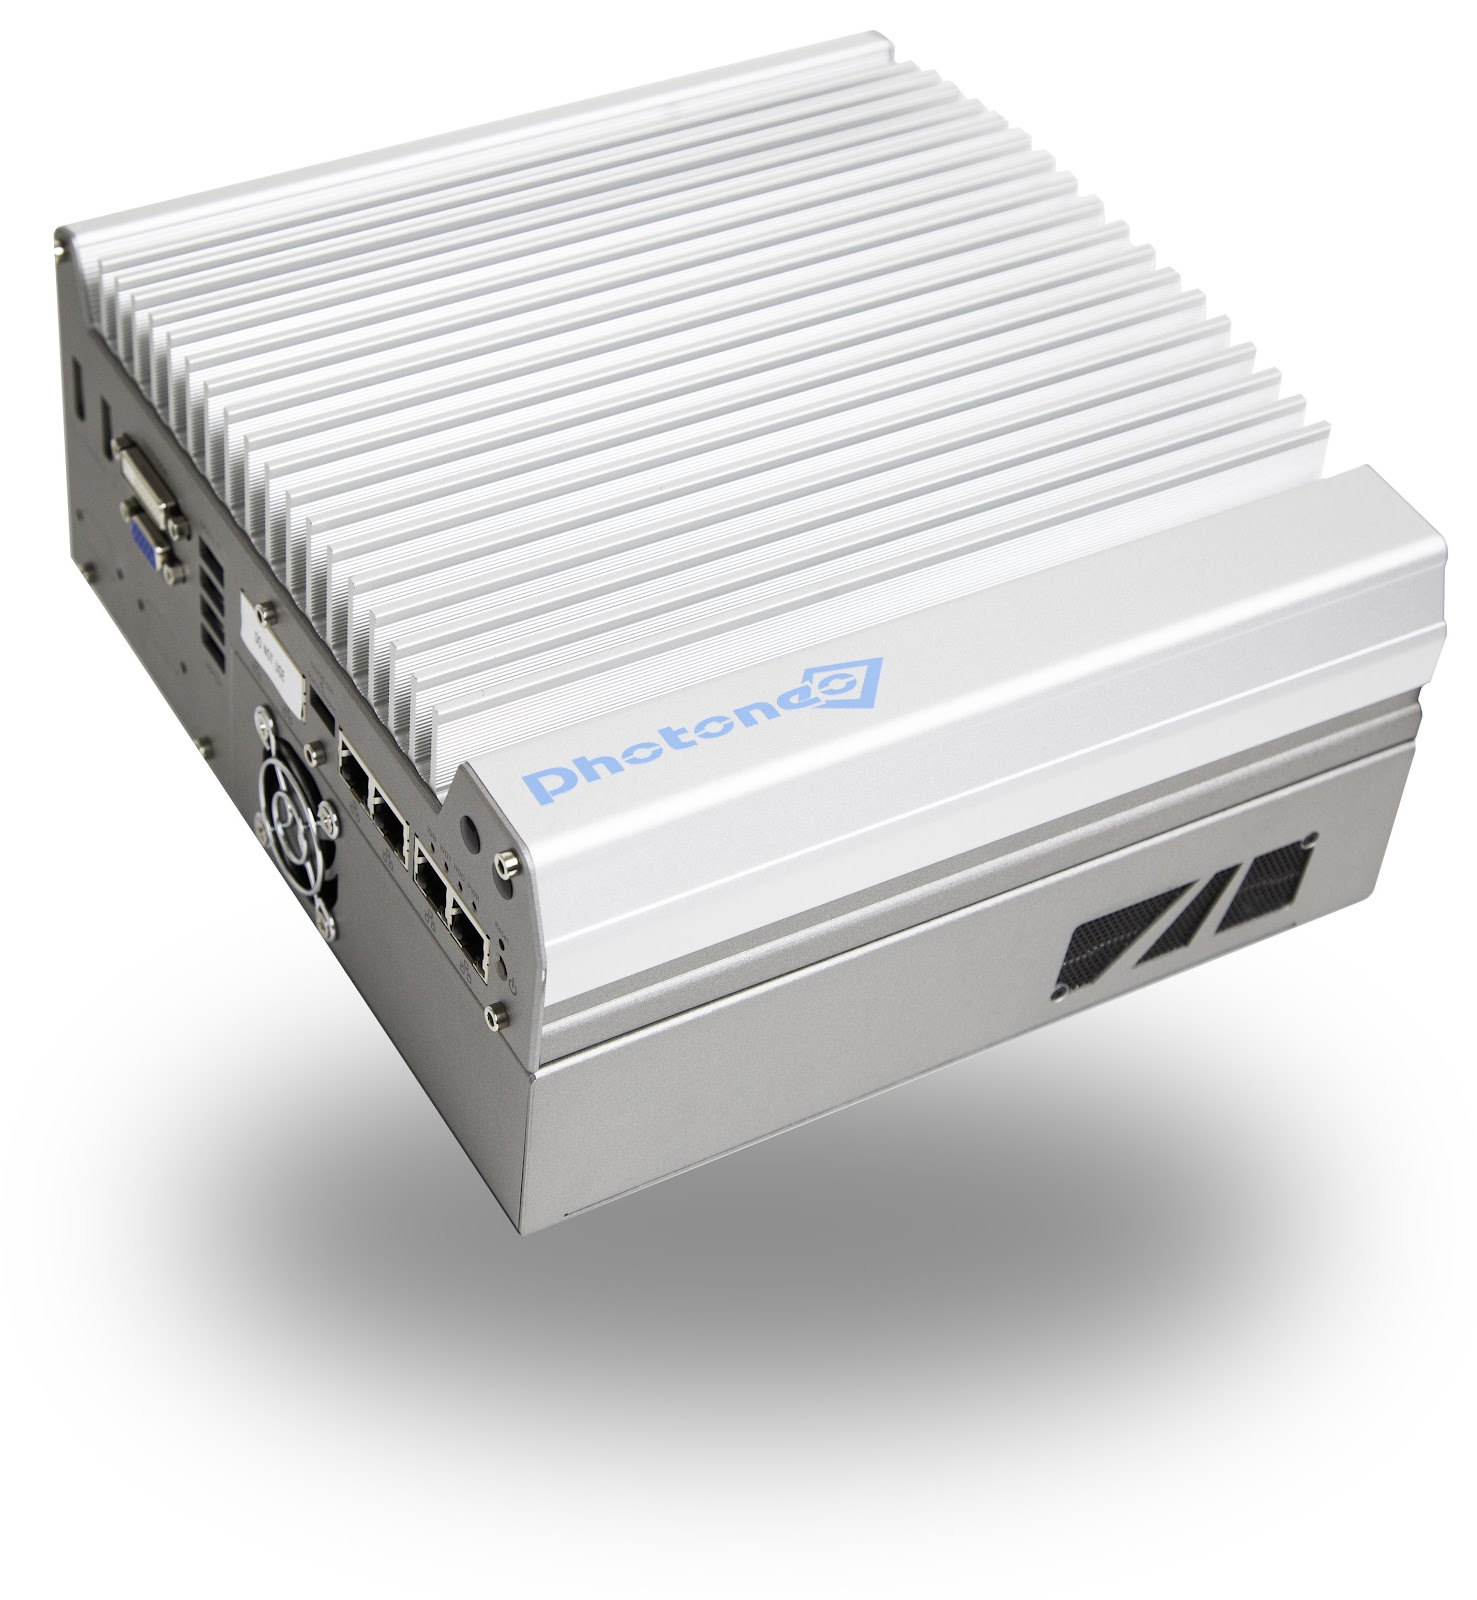
\includegraphics[width=4cm]{Thesis-report/Figures/vision controller.png}
    \caption{Vision Controller \cite{ref2}}
    \label{fig:vision-controller}
\end{figure}
The vision controller is connected to a pC through the web interface to trigger the camera and see the Web interface for communication.To connect the 3D sensor, gigabit Ethernet connections of Cat5e or above are needed.  multiple 3D sensors can be connected using a gigabit switch.  multiple 3D sensors can be connected using a gigabit switch. The Ethernet connection from the switch or 3D sensor is linked to the scanner's physical network port in both scenarios. To visualize 3D scans, calibrate robot cameras, and establish localization settings, a connection to the 3D sensor is required.To set up the network interface that the vision controller uses to connect to the photoneo 3D sensor(s), enter the Network page and select the Scanner Interface section. Both a fixed IPv6 link-local address and a programmable IPv4 address are features of photoneo 3D sensors.\cite{ref15}

\subsection{Marker pattern}
\begin{figure}[h]
    \centering
    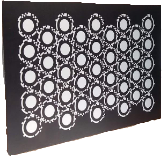
\includegraphics[width=4cm]{Thesis-report/Figures/marker_pattern.png}
    \caption{Marker pattern \cite{ref2}.}
    \label{fig:marker-pattern}
\end{figure}

Figure \ref{fig:marker-pattern} above shows the S30 calibration board that helps calibrate the conveyor belt, which aligns the coordinates of the object with the conveyor belt for objects passing through the belt. To enable the robot to retrieve objects from the moving conveyor belt, the belt can be used to align the object coordinates with the conveyor belt\cite{ref2}.

\subsection{Active ambient light rejection}
The inability of all area-based 3D sensors to function in direct sunshine is a typical problem.  Direct sunshine has a maximum power output of 1120 W/m³. High-end band-pass filters installed in all of photoneo's sensors lower ambient light levels to around 15 W/m².  Although it can oversaturate the image or produce high shot noise, this still performs better than the majority of projection systems.

Delivering active lighting as a brief pulse, which raises the projection's optical power output and shortens the system's exposure time overall, is one way to lessen the impact of ambient light.  This method has drawbacks, such as limited parts availability, complicated power supply management, hazards to eye safety, or problems with heat control\cite{ref15}.

The sensor and projection can cooperate to regulate the light sensitivity of the sensor surface through active ambient light suppression. The direct reflection of the projection at any one time during the acquisition may only reveal about 1 percent of the sensor surface due to geometrical constraints.  The remaining 99 percent of the sensor can be turned off by the camera's control circuit, preventing any photoelectrons from being collected.  Scanning in direct sunshine is made possible by the technology's efficient 1:100 suppression of ambient light from any source (key benefit 5)\cite{ref15}.

The same method significantly reduces internal reflections between pixels at the same 1:100 ratio (important advantage 6).  The technique rejects the second scanner's projection in 99 percent of the image when two sensors are working in the same area at the same time, affecting only 1 percent of the pixels. It is simple to recognize and remove these pixels from the output (key advantage 7)\cite{ref15}.
 
\begin{figure}[h]
    \centering
    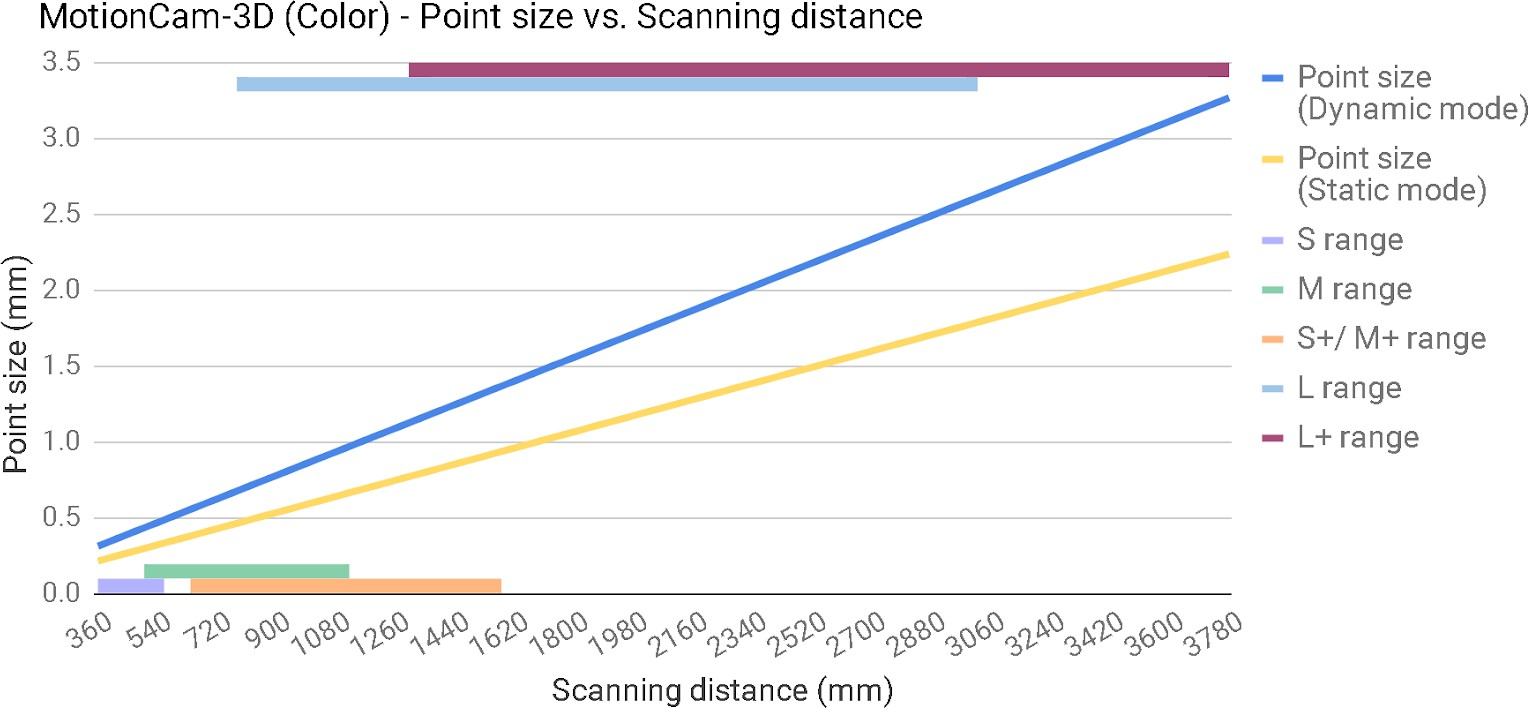
\includegraphics[width=12cm]{Thesis-report/Figures/scanningdistance.jpg}
    \caption{Point Size vs. Scanning Distance \cite{ref15}}
    \label{fig:scanning-distance}
\end{figure}

Figure 15 below shows the scanning distance of various cameras vs. their point size. The m+ Range camera has been utilized in this instance \cite{ref15}. 

\newpage
\subsection{Object for picking}
We have used a trapezoid for object picking 

\begin{figure}[h]
    \centering
    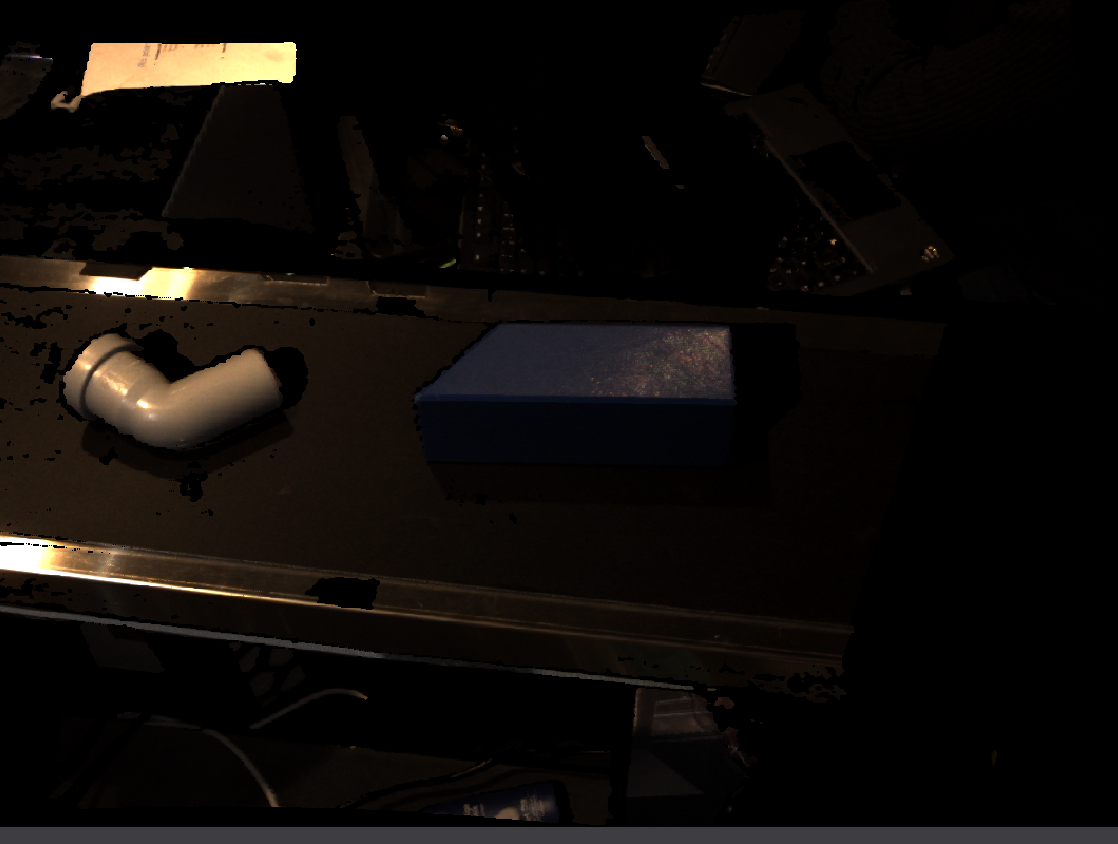
\includegraphics[width=4cm]{Thesis-report/Figures/two.png} 
    \caption{Trapezoid}
    \label{fig1:two}
\end{figure}

\subsubsection{Trapezoid}
The trapezoid  is:\\
\begin{figure}
\centering
\begin{minipage}{0.58\textwidth} % Adjust width as needed
    \centering
    \includegraphics[width=6.5cm]{Thesis-report/Figures/trapezoid_stl.jpg} 
    \caption{STL file for Trapezoid object}
    \label{fig:trapezoid_stl}
\end{minipage}
\hfill
\begin{minipage}{0.28\textwidth} % Adjust width as needed
    \centering
    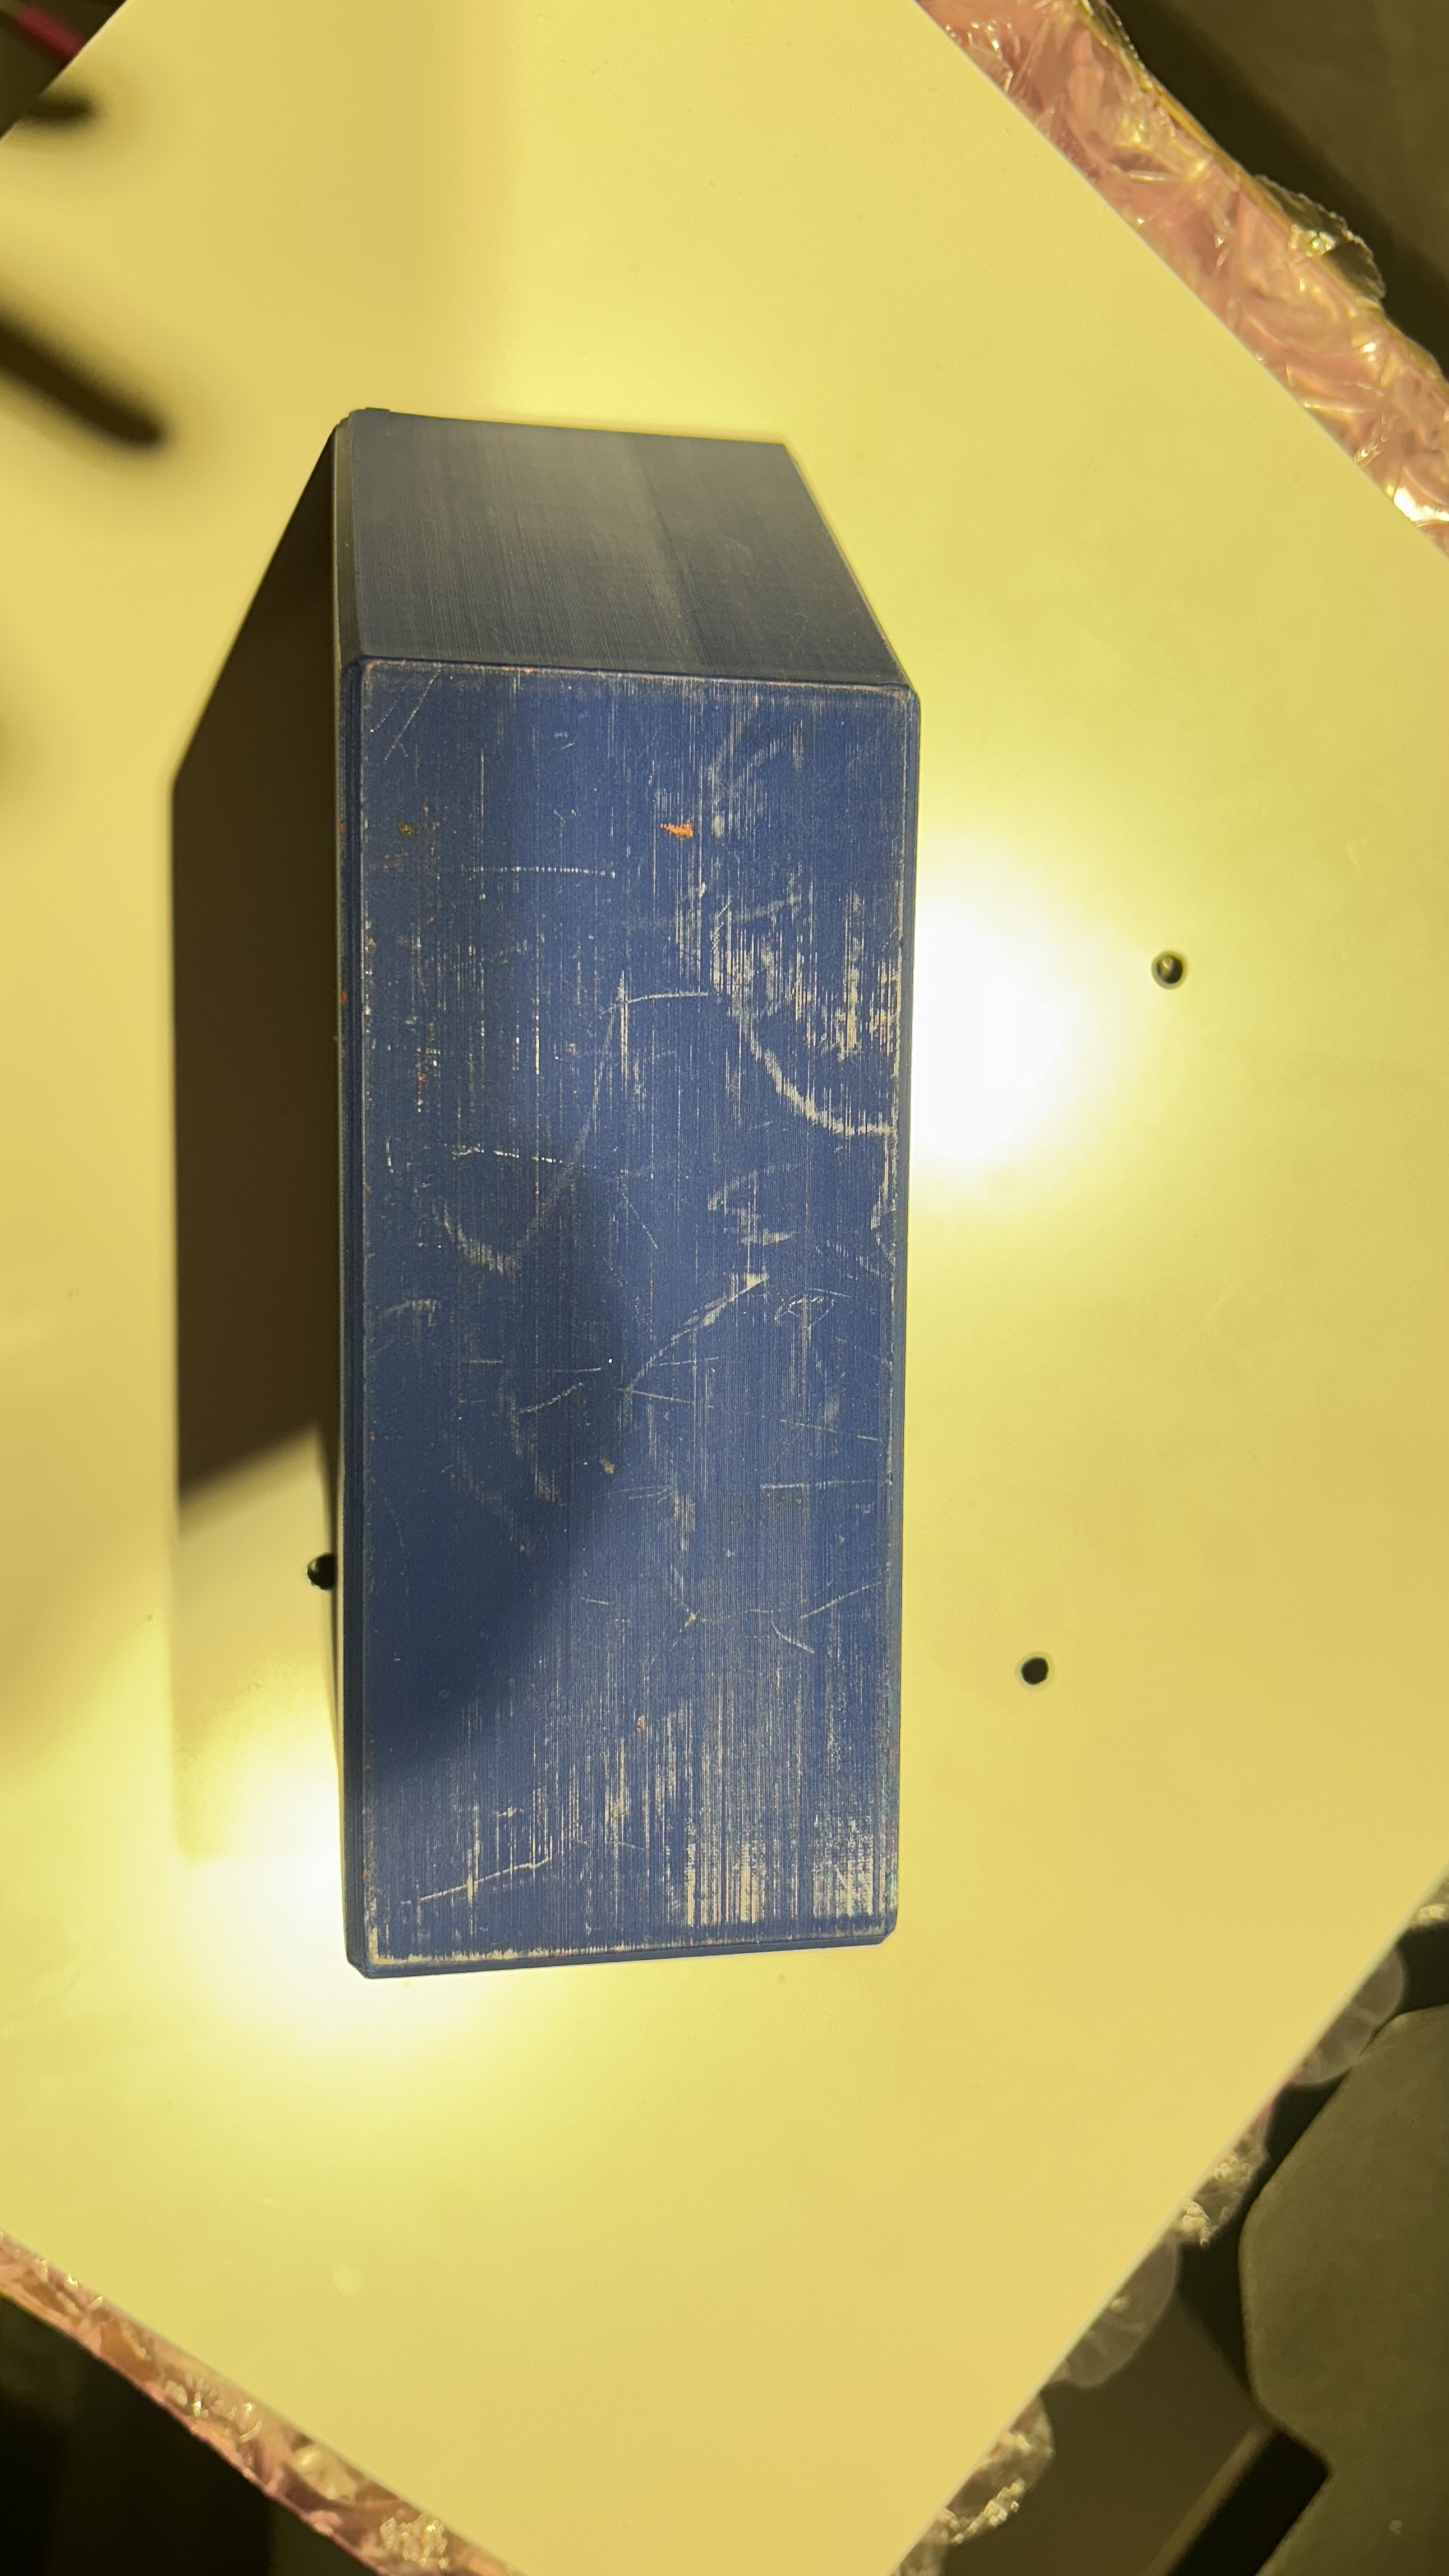
\includegraphics[width=3cm]{Thesis-report/Figures/trapezoid.png} \caption{Trapezoid object}
    \label{fig:trapezoid}
\end{minipage}
\end{figure}
The figure above shows the STL file of the trapezoid, which is used to pick up the object. While loading the STL file for the object, we will get the X, Y, and Z coordinates for the object.

\subsection{Camera Examples Under Different Settings}

The following figures illustrate examples of the same object captured under various camera settings.

\noindent\textbf{1. Texture} The texture image helps ensure that object details appear natural and are visually understandable.
\begin{figure}[H]
    \centering
    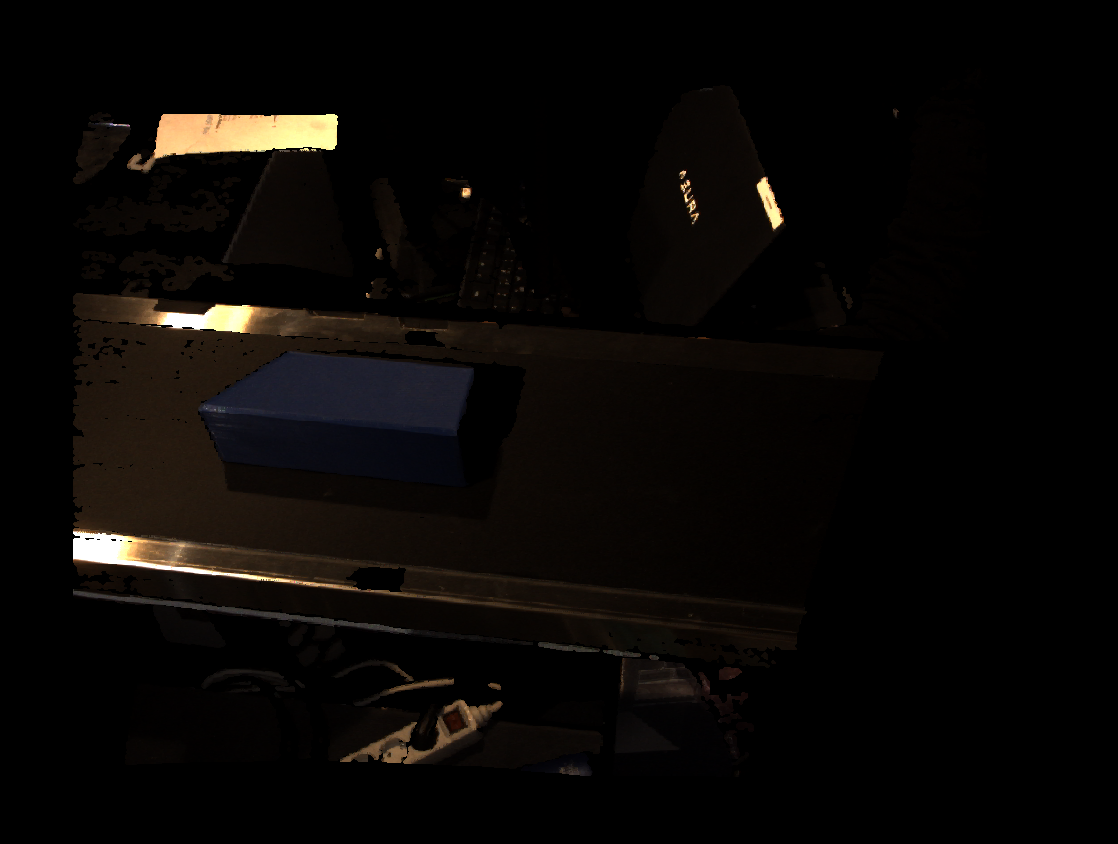
\includegraphics[width=6cm]{Thesis-report/Figures/new_Texture.png}
    \caption{Texture}
    \label{fig:texture}
\end{figure}

\noindent\textbf{2. Event map} The event map captures fast-moving objects without motion blur and ensures full frames at a fixed rate.
\begin{figure}[H]
    \centering
    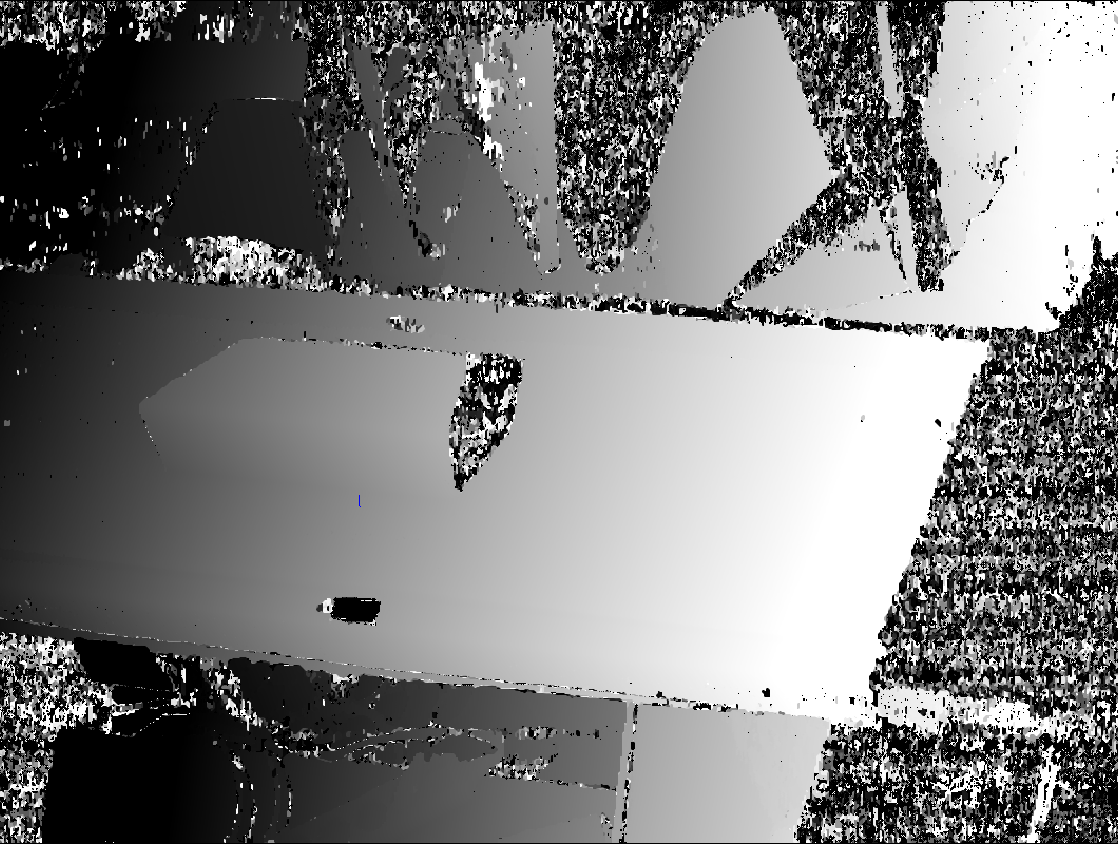
\includegraphics[width=6cm]{Thesis-report/Figures/new_EventMap.png}
    \caption{Event map}
    \label{fig:eventmap}
\end{figure}

\noindent\textbf{3. Depth map (Grayscale)} The grayscale depth map stores complex 3D coordinates, where brighter pixels represent closer distances and darker pixels represent farther ones.
\begin{figure}[H]
    \centering
    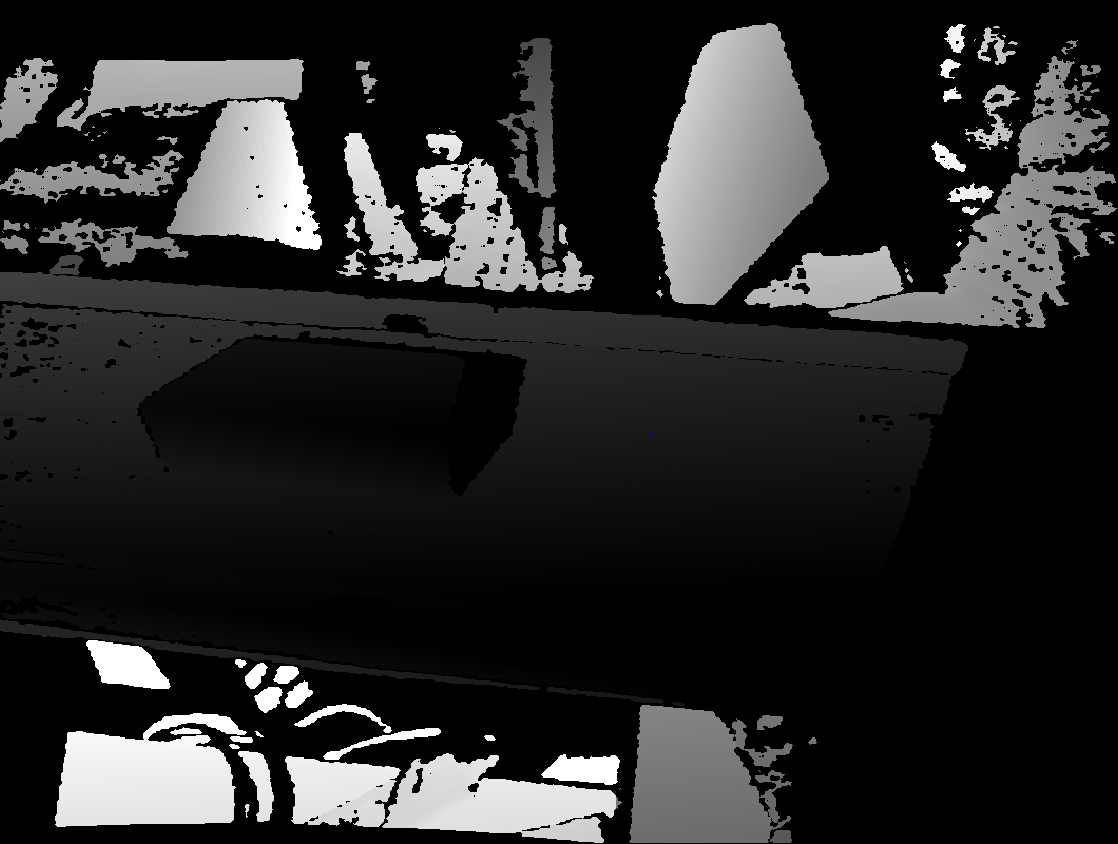
\includegraphics[width=6cm]{Thesis-report/Figures/new_DepthMap.png}
    \caption{Depth map (Grayscale)}
    \label{fig:depthmap_gray}
\end{figure}

\noindent\textbf{4. Depth Hue} Depth Hue provides a more intuitive and visually distinct way to represent depth compared to grayscale.
\begin{figure}[H]
    \centering
    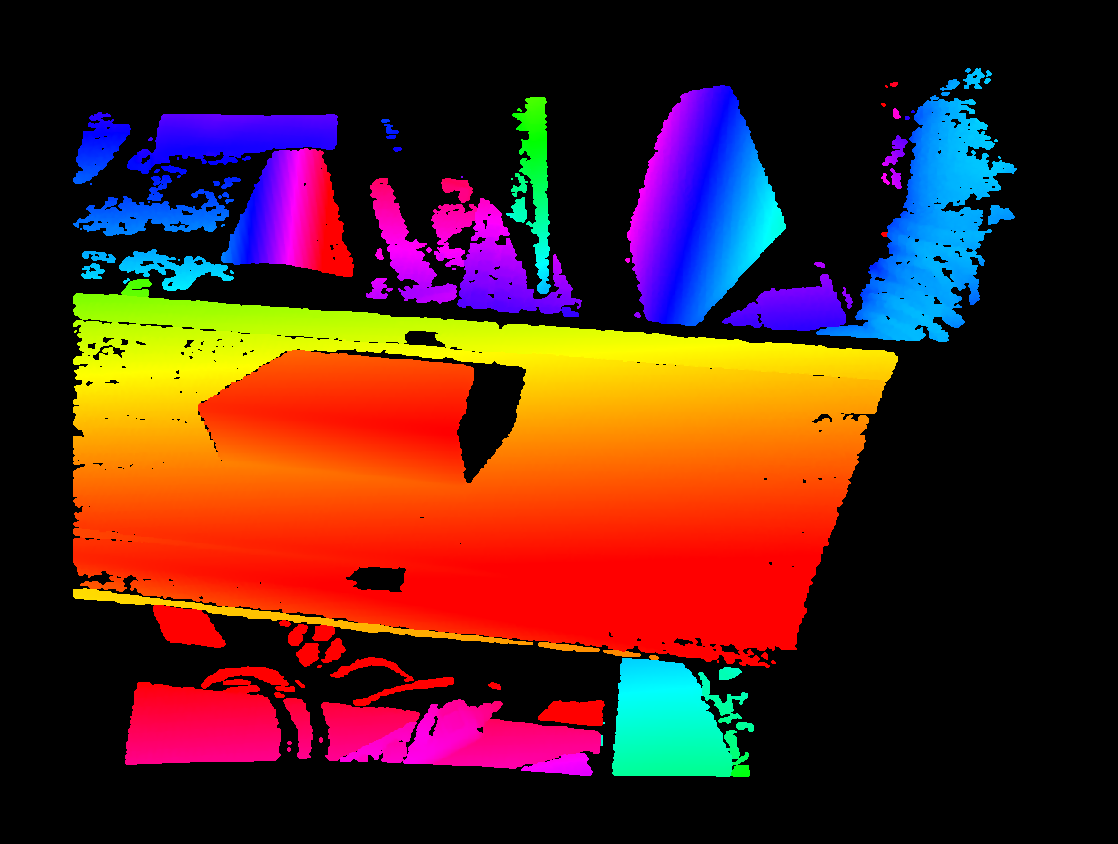
\includegraphics[width=6cm]{Thesis-report/Figures/new_Depth_Hue.png}
    \caption{Depth Hue}
    \label{fig:depth_hue}
\end{figure}

\noindent\textbf{5. Confidence map} The confidence map indicates the reliability of the captured depth or image data, helping to filter out noisy and unreliable regions.
\begin{figure}[H]
    \centering
    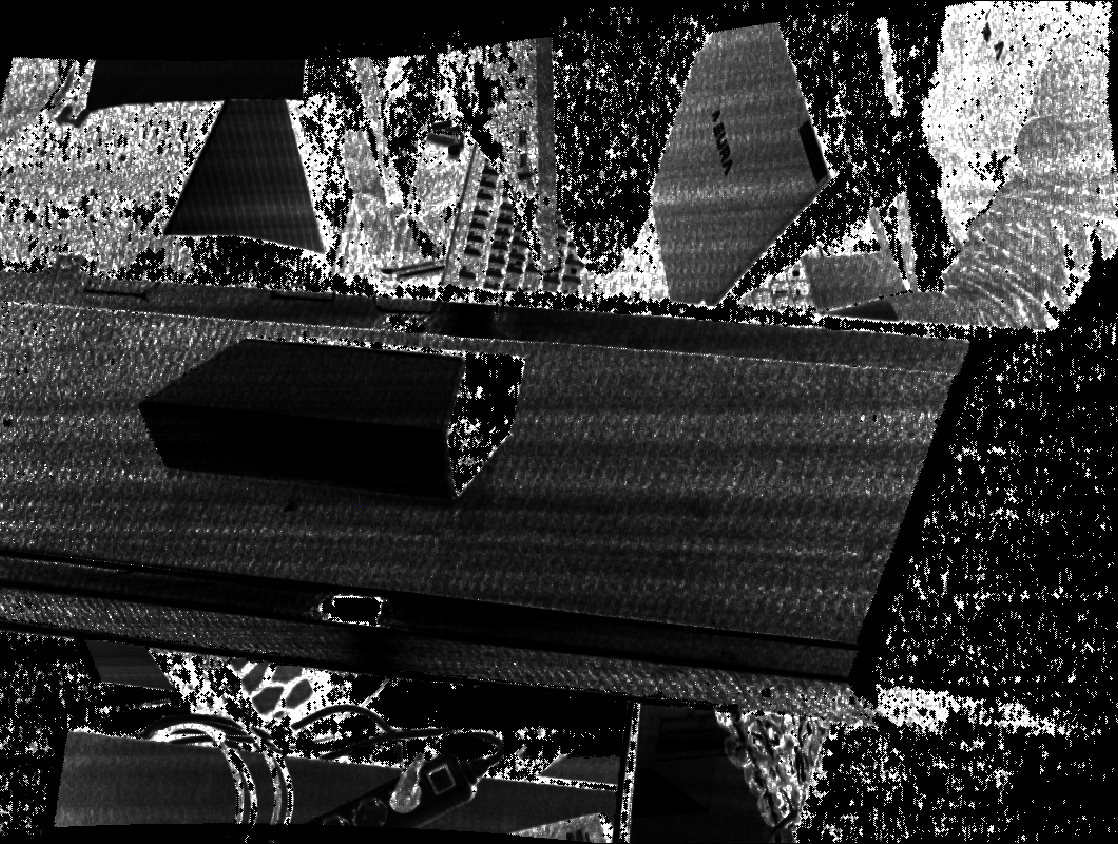
\includegraphics[width=6cm]{Thesis-report/Figures/new_ConfidenceMap.png}
    \caption{Confidence map}
    \label{fig:confidence_map}
\end{figure}

\noindent\textbf{6. Normals} Surface normals are essential for realistic rendering and understanding object orientation. They describe how surfaces interact with light, which is crucial in graphics and computer vision.
\begin{figure}[H]
    \centering
    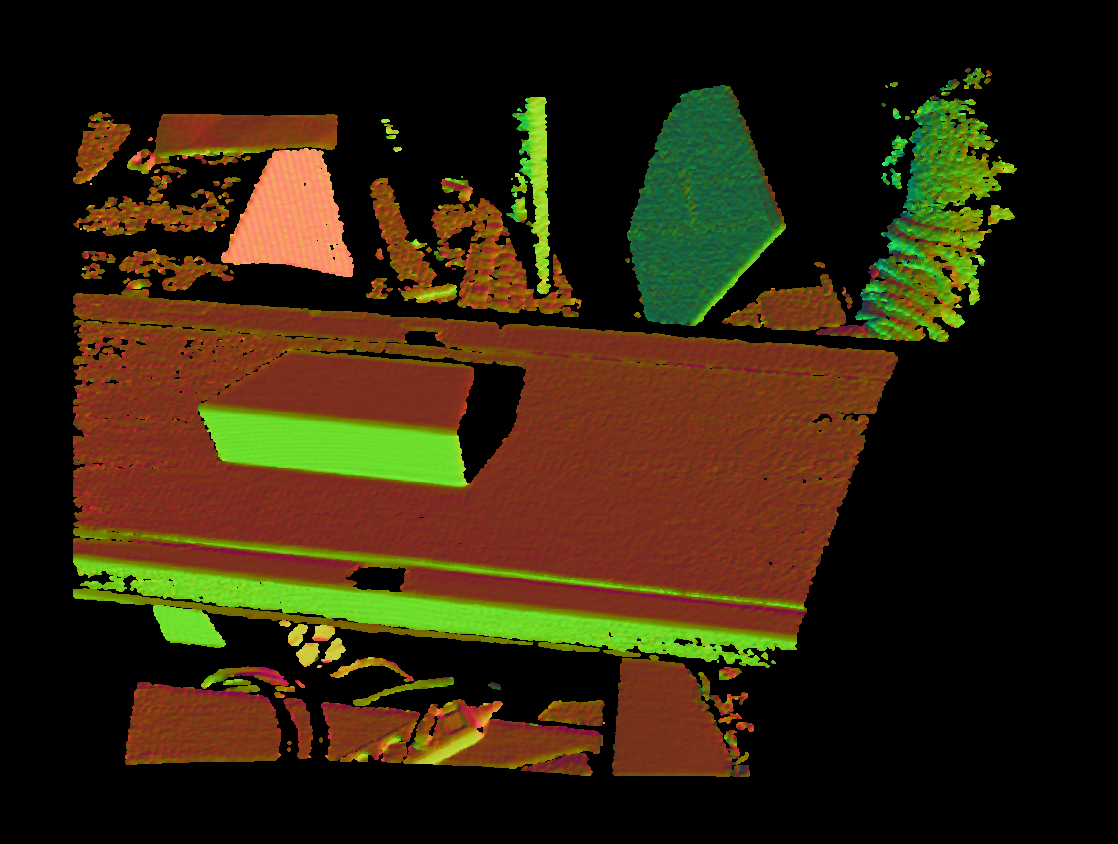
\includegraphics[width=6cm]{Thesis-report/Figures/new_Normals.png}
    \caption{Normals}
    \label{fig:normals}
\end{figure}

\noindent\textbf{7. White Illumination} White light illumination is used to uniformly light the object for color and texture accuracy.
\begin{figure}[H]
    \centering
    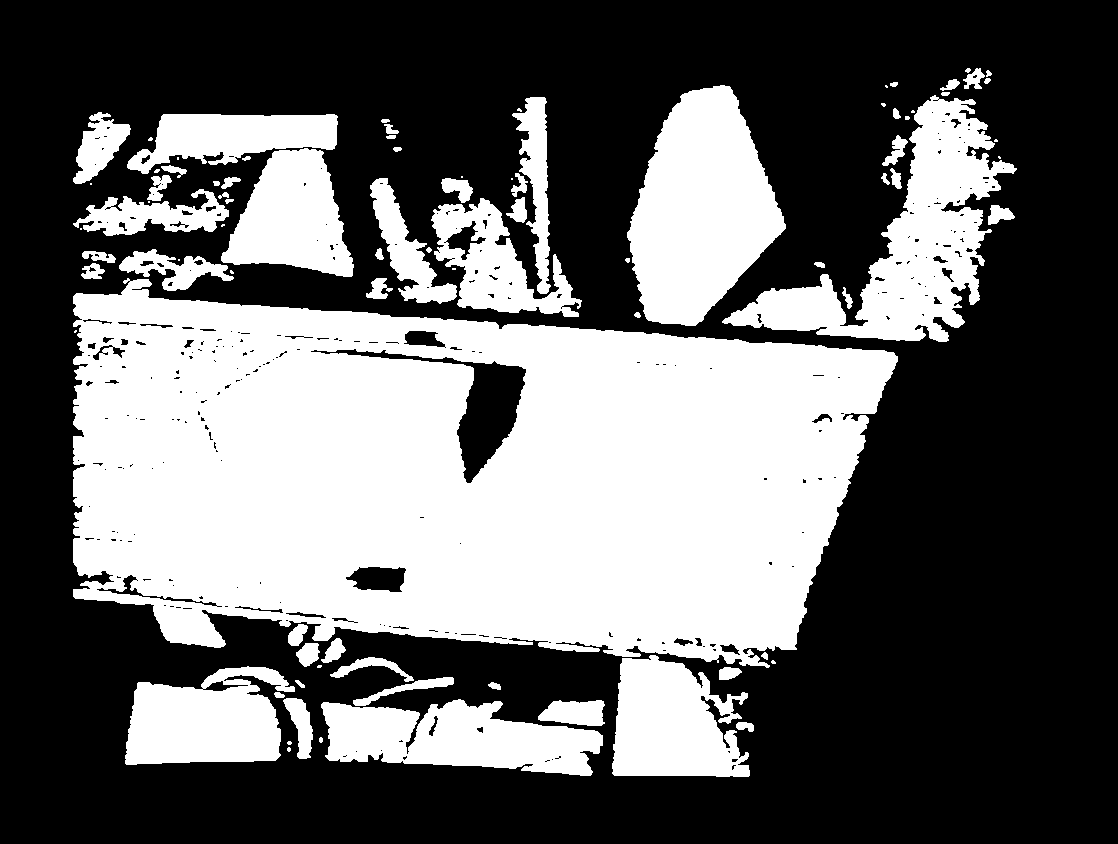
\includegraphics[width=6cm]{Thesis-report/Figures/new_white.png}
    \caption{White Illumination}
    \label{fig:white}
\end{figure}

\noindent\textbf{8. Color Image} In computer vision applications, color images offer the rich visual information required for object recognition, segmentation, and rendering.
\begin{figure}[H]
    \centering
    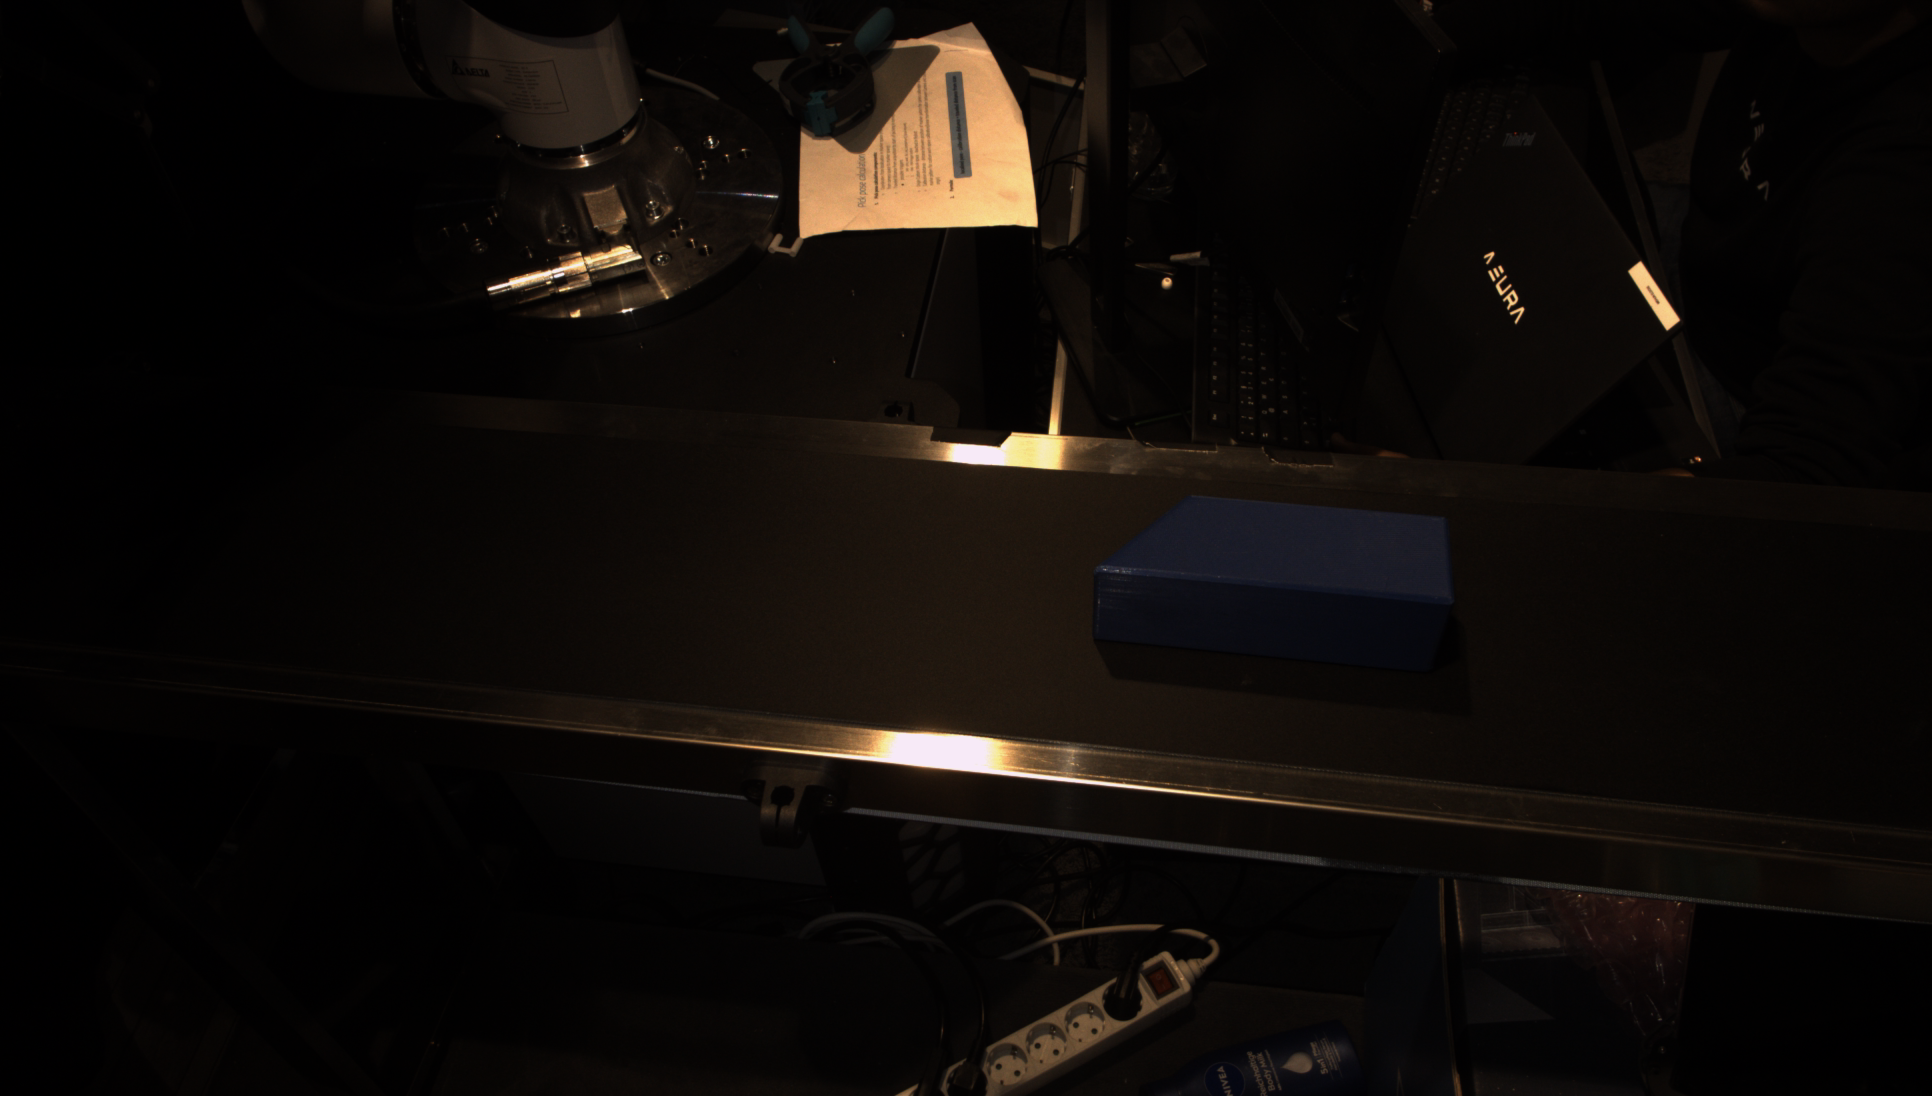
\includegraphics[width=6cm]{Thesis-report/Figures/new_white_IMG_ColorCameraImage_8Bit.png}
    \caption{Color Image}
    \label{fig:color_image}
\end{figure}
\newpage
\subsubsection{Conveyor Belt}

The conveyor belt is the main belt where we have to place the object, thereby putting the object into dynamic mode \cite{ref22}. \\

The conveyor belt specification includes\\
\begin{enumerate}
    \item The item model has Belt size: 59x7.8 in/1498.6x198 mm \cite{ref22}
    \item Table Width: 9.9 in/252mm \cite{ref22}
    \item Load Capacity Limit: 82.67 lbs/37.5 kg \cite{ref22}
    \item material: 201 Stainless Steel \cite{ref22}
    \item product Weight: 40.79/18.5 kg \cite{ref22}
    \item Conveyor belt speed: Bi-directional Variable speed, 28 m/min \cite{ref22}
    \item product Size: 58.86 x 14.17 x 35.91 in/1495 x 360 x 912 mm \cite{ref22}
\end{enumerate}

\begin{figure}[h]
    \centering
{
        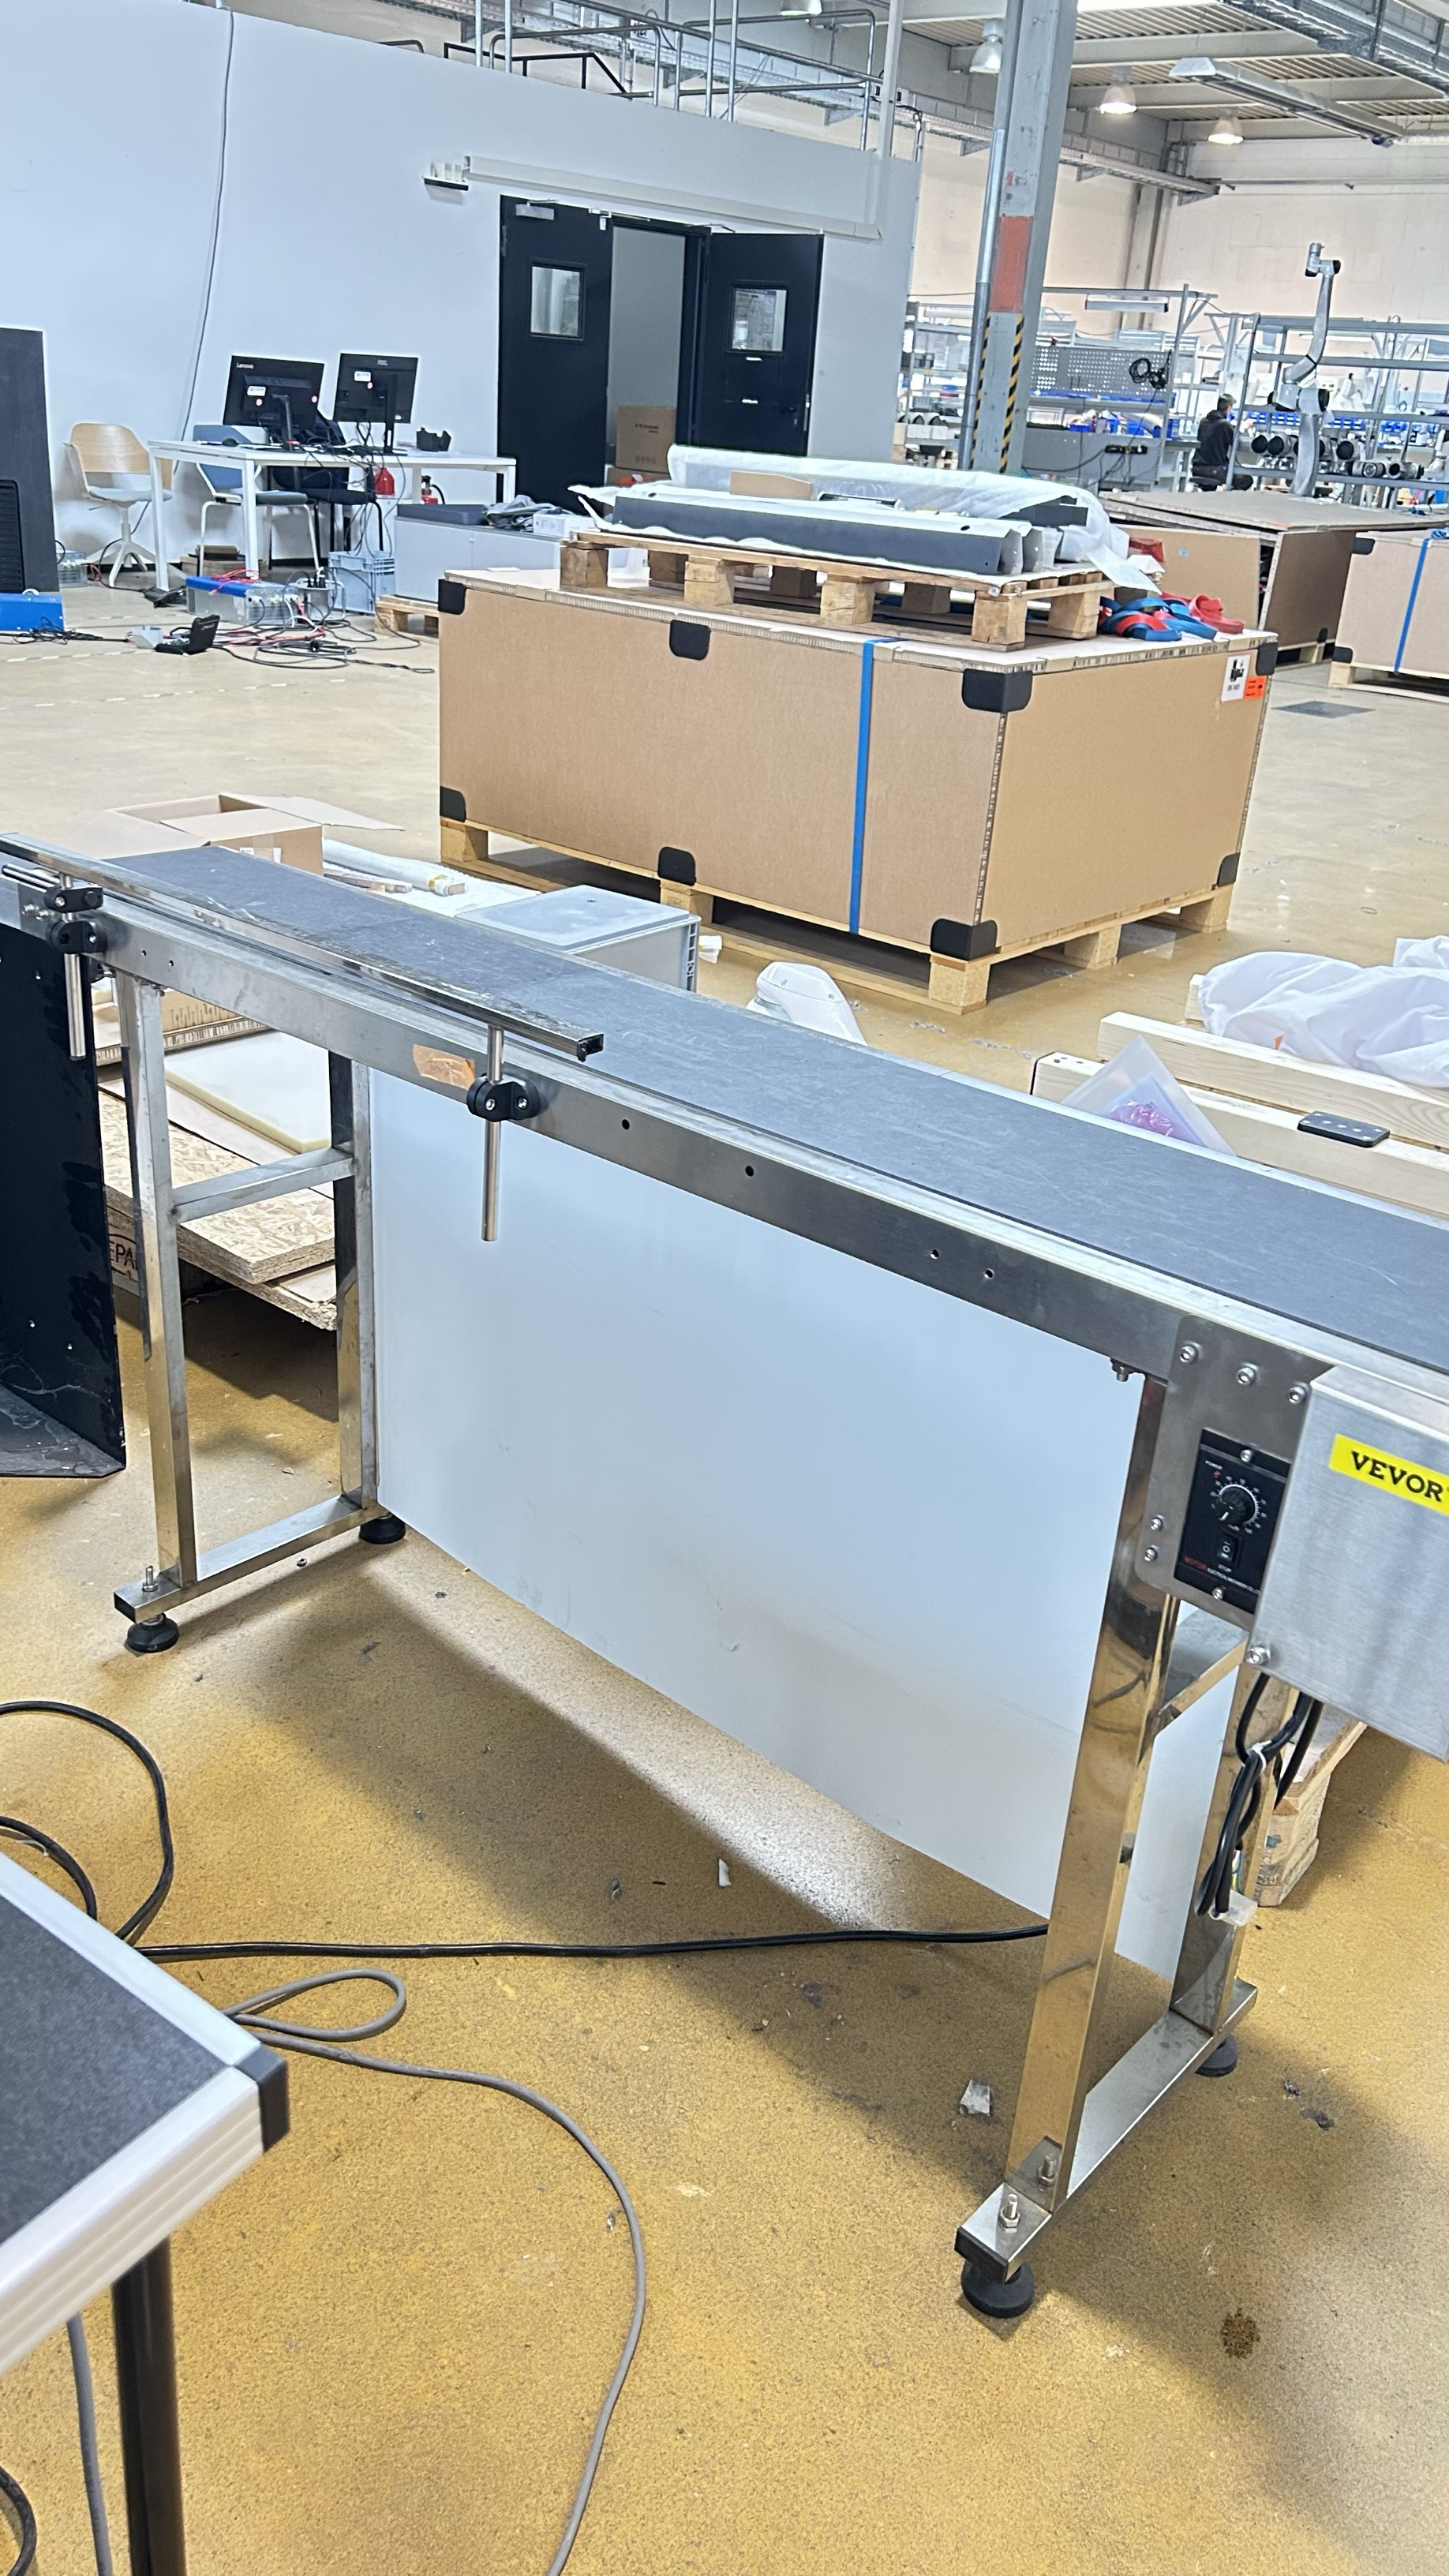
\includegraphics[width=5cm] {Thesis-report/Figures/CV belt1.jpeg}
        \label{fig:cv_belt1}
    }
    \quad
{
        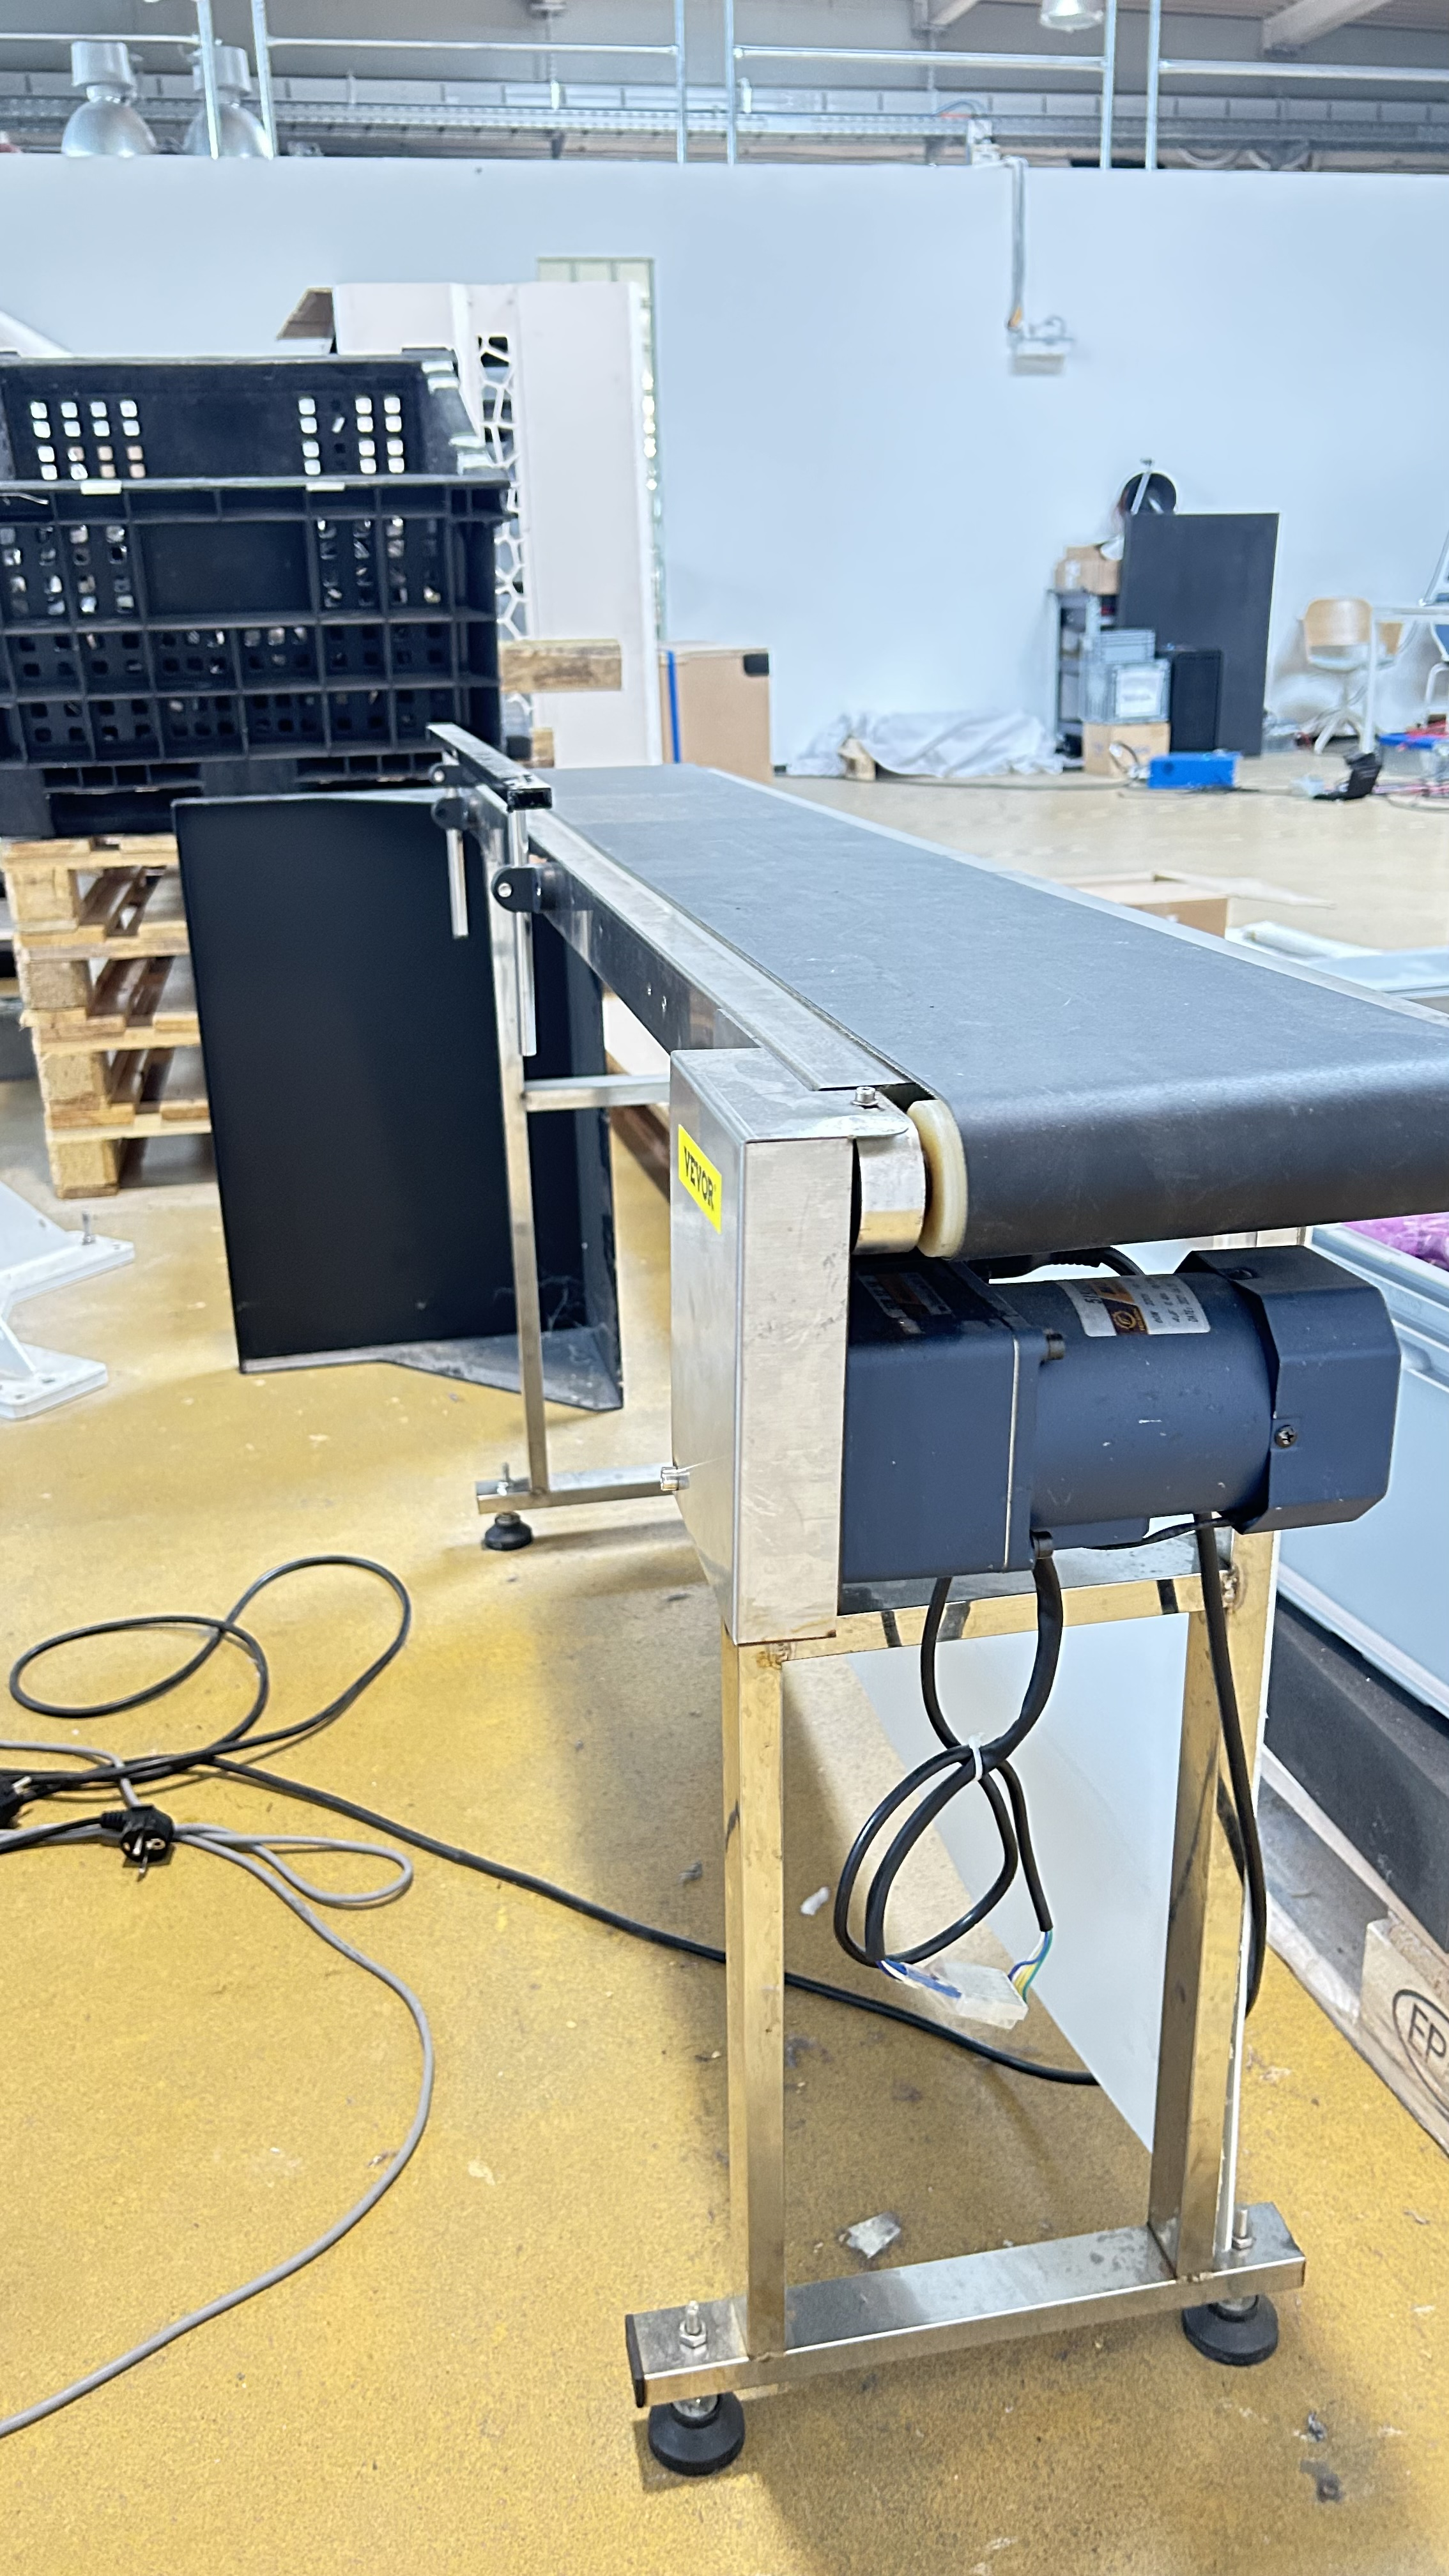
\includegraphics[width=5cm]{Thesis-report/Figures/CV_ belt2.jpeg}
        \label{fig:cv_belt2}
    }
    \caption{Images of the conveyor belt}
    \label{fig:conveyor_belt}
\end{figure}

The components are depicted in the following picture and include:


1. \textbf{Conveyor Belt} The primary surface for moving goods or commodities from one location to another is the conveyor belt.  It efficiently transports objects of all shapes and sizes and always operates when the engine is turned on \cite{ref22}.\\



2.	\textbf {Adjustment Lever}
Function: This lever allows for adjustment of the conveyor system.  To ensure smooth operation and accommodate different materials, it can be utilized to modify the belt's height, alignment, or tension \cite{ref22}.

3.	\textbf {Guardrail}
Function: To stop goods from slipping off the conveyor belt while in transportation, guardrails are positioned along its edges.  It facilitates the safe movement of goods down the belt, especially when handling uneven or slippery objects \cite{ref22}.\\

4.	\textbf {Motor}
Function: It drives the belt by converting electrical energy into mechanical energy, either directly or through a gearbox and pulleys \cite{ref22}. \\
\begin{figure}[h]
    \centering
    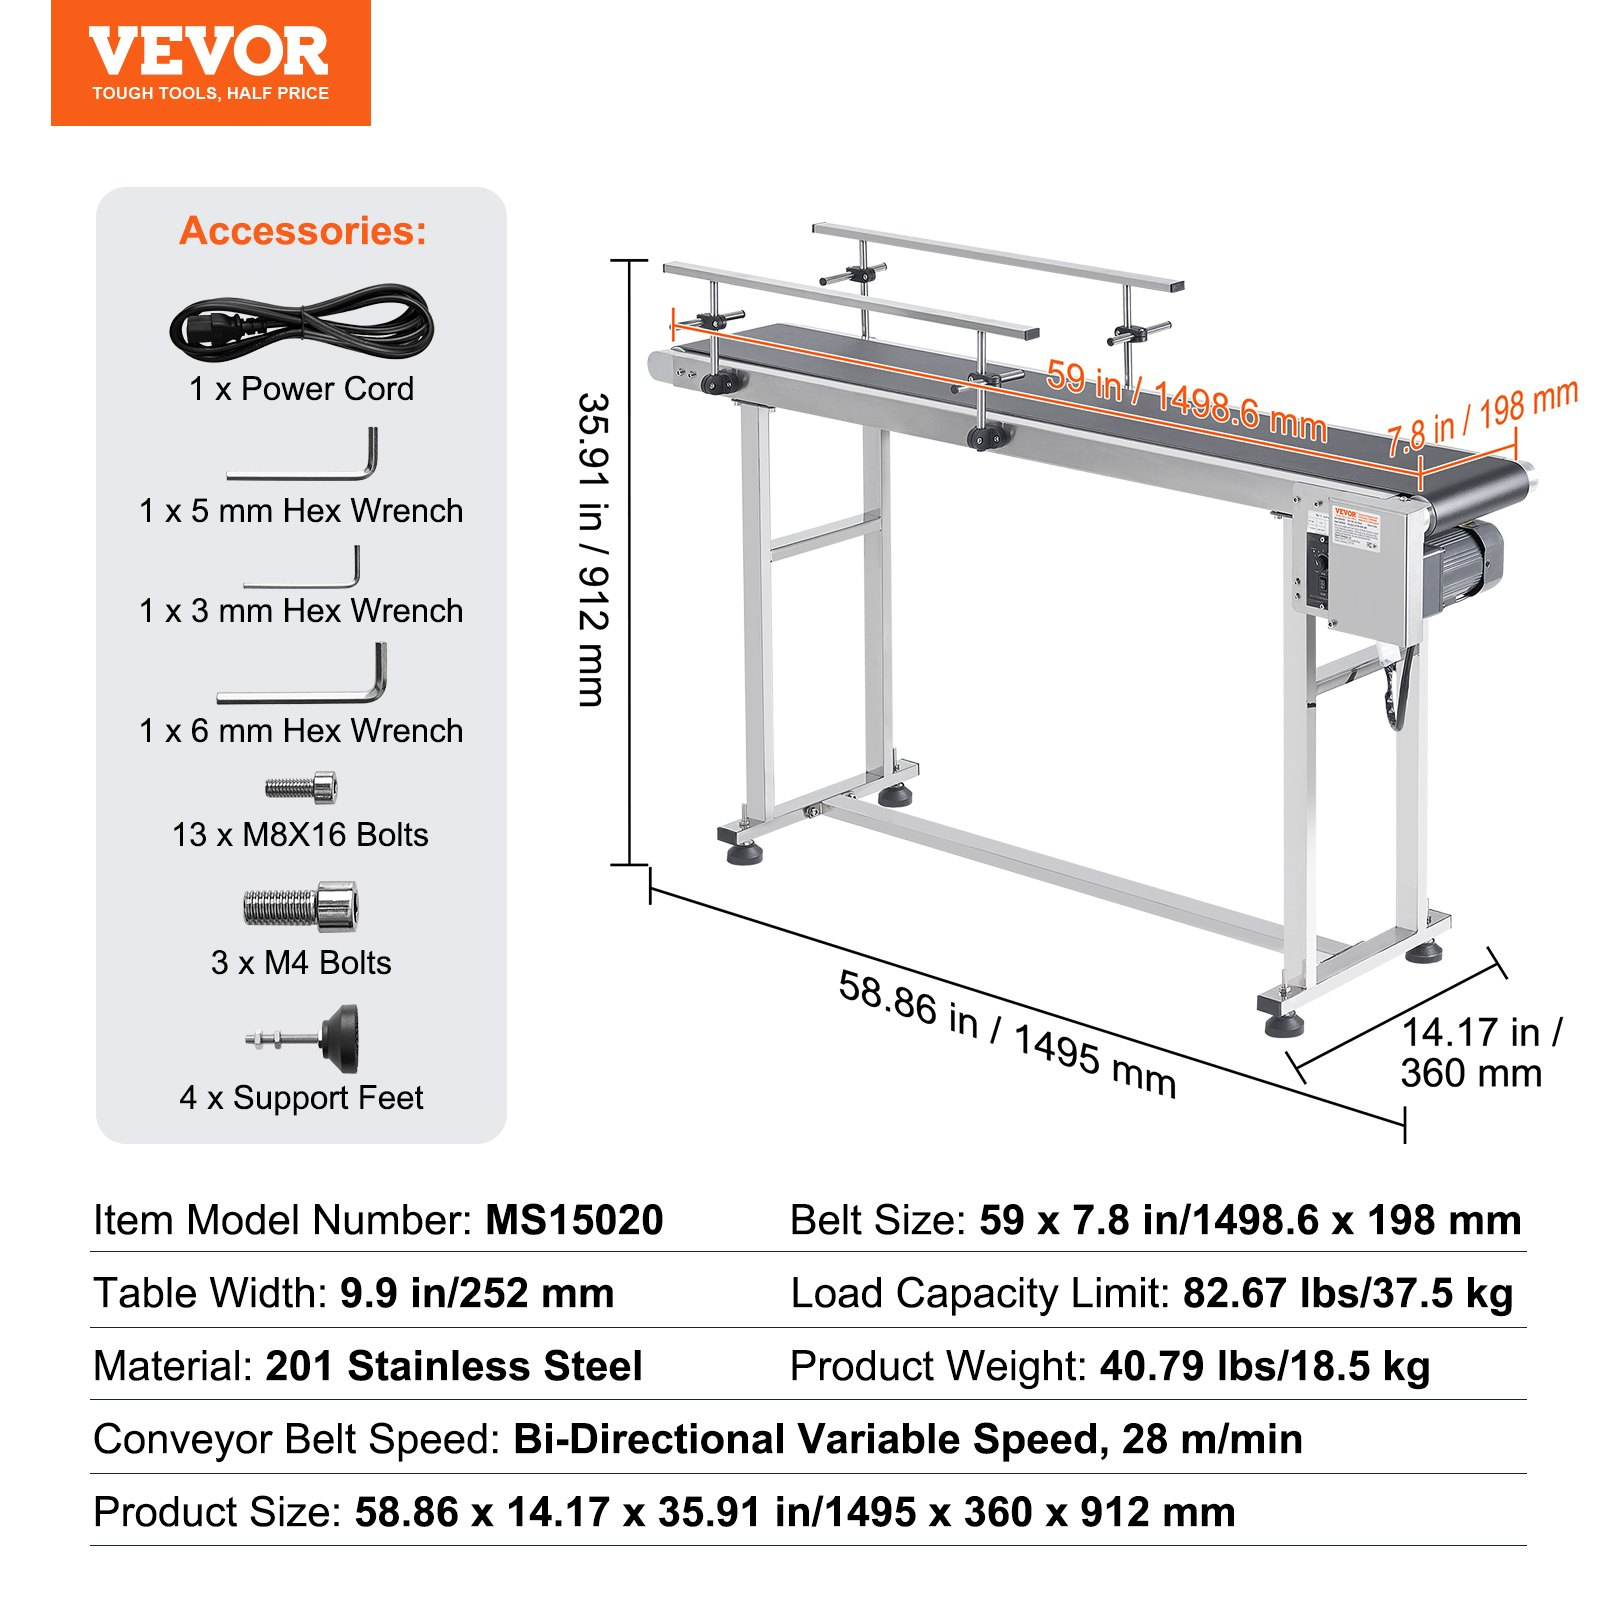
\includegraphics[width=6cm]{Thesis-report/Figures/belt_dimension.jpg}
    \caption{Conveyor belt with Details\cite{ref22}}
    \label{fig1:conveyor-belt-with-details}
\end{figure}

5.	\textbf {Control panel}
Function: Operators can oversee the conveyor's operation from the control panel. Switches, speed controls, emergency stop buttons, and other controls to modify the conveyor's direction, speed, and mode of operation may be included \cite{ref22}. \\

6.	\textbf{Rubber Feet}
Function: The rubber feet steady the conveyor system and assist in absorbing vibrations while it is in use.  Additionally, they shield the floor from scuffs and stop the conveyor from slipping on smooth surfaces, which could lead to motion detection instability\cite{ref22}.\\

\begin{figure}[h]
    \centering
    \includegraphics[width=3cm]{Thesis-report/Figures/cvdimension.jpg}
    \caption{Conveyor belt with Dimensions\cite{ref22}}
    \label{fig:cv-dimension}
\end{figure}

\section{Methodology}

This approach uses an interactive route planning solution for a fixed-based manipulator from an initial to a final configuration, along with a camera system for 3D detection.  Two characteristics of the ideal path should be collision-free and metric minimization.\\
The flowchart below represents the basic topics that we are going to discuss:
\begin{figure}[H]  % requires \usepackage{float}
  \centering
  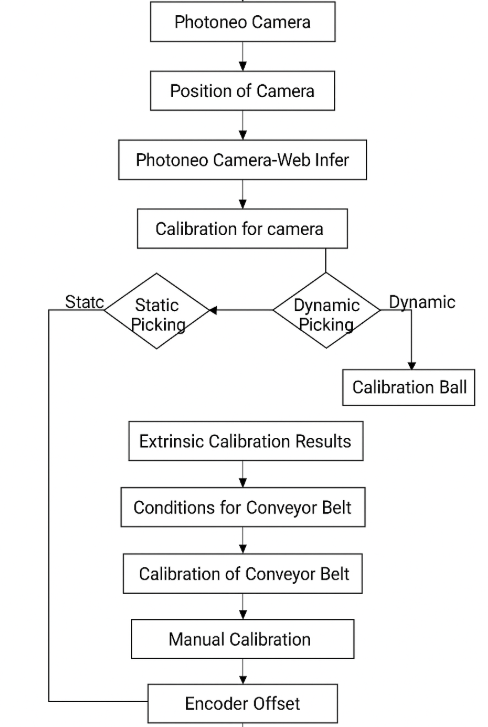
\includegraphics[width=6cm]{Thesis-report/Figures/Methodology.png}
  \caption{Methodology Flowchart \cite{ref18}}
  \label{fig:methodology}
\end{figure}

Surface imaging and geometry estimation are the two primary subtasks that comprise imaging of the item to be inspected. There are numerous ways to implement automated optical inspection systems in the field of optical inspection. The choice of an efficient set of tactics should be guided by the task at hand. Improving the contrast between an object's flawed and perfect areas is crucial for dependable and robust automated detection systems in the field of optical surface inspection.

\subsection{Photoneo Camera}


The camera we have used to track the moving object's motion through the conveyor belt is a 
MotionCam 3D m+, which has advanced settings that can capture and detect the object's position. The photoneo camera mainly consists of 3D sensing technology, which contains parallel structured light that helps provide the light source to detect objects \cite{ref2}.\\

Accurate point clouds and a standard intensity image of the object can be captured by this camera.  Its foundation is a customized CMOS image sensor that utilizes photoneo's patented parallel Structured Light technology\cite{ref15}.

\begin{figure}[h]
    \centering
    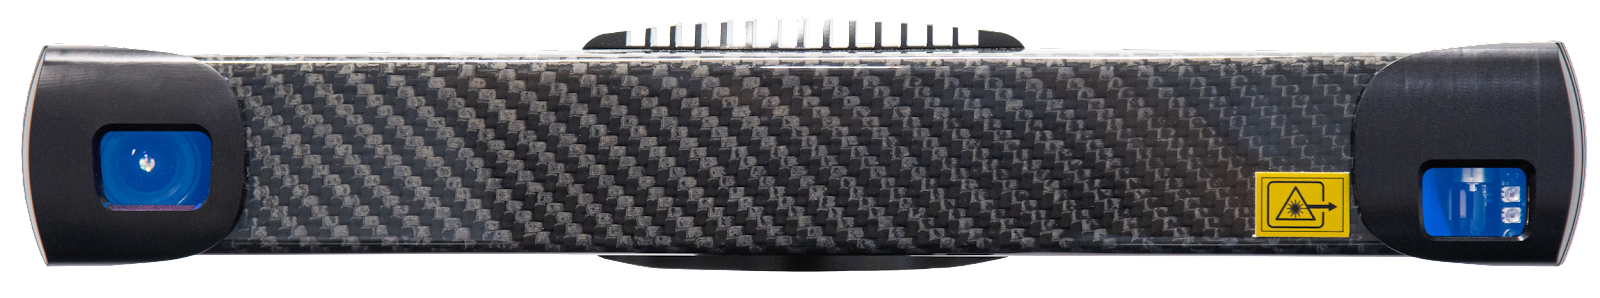
\includegraphics[width=5cm]{Thesis-report/Figures/CAMERA.png}
    \caption{Photoneo Camera \cite{ref2}} 
    \label{fig:Photoneo-camera}
\end{figure}

\begin{figure}[h]
    \centering
    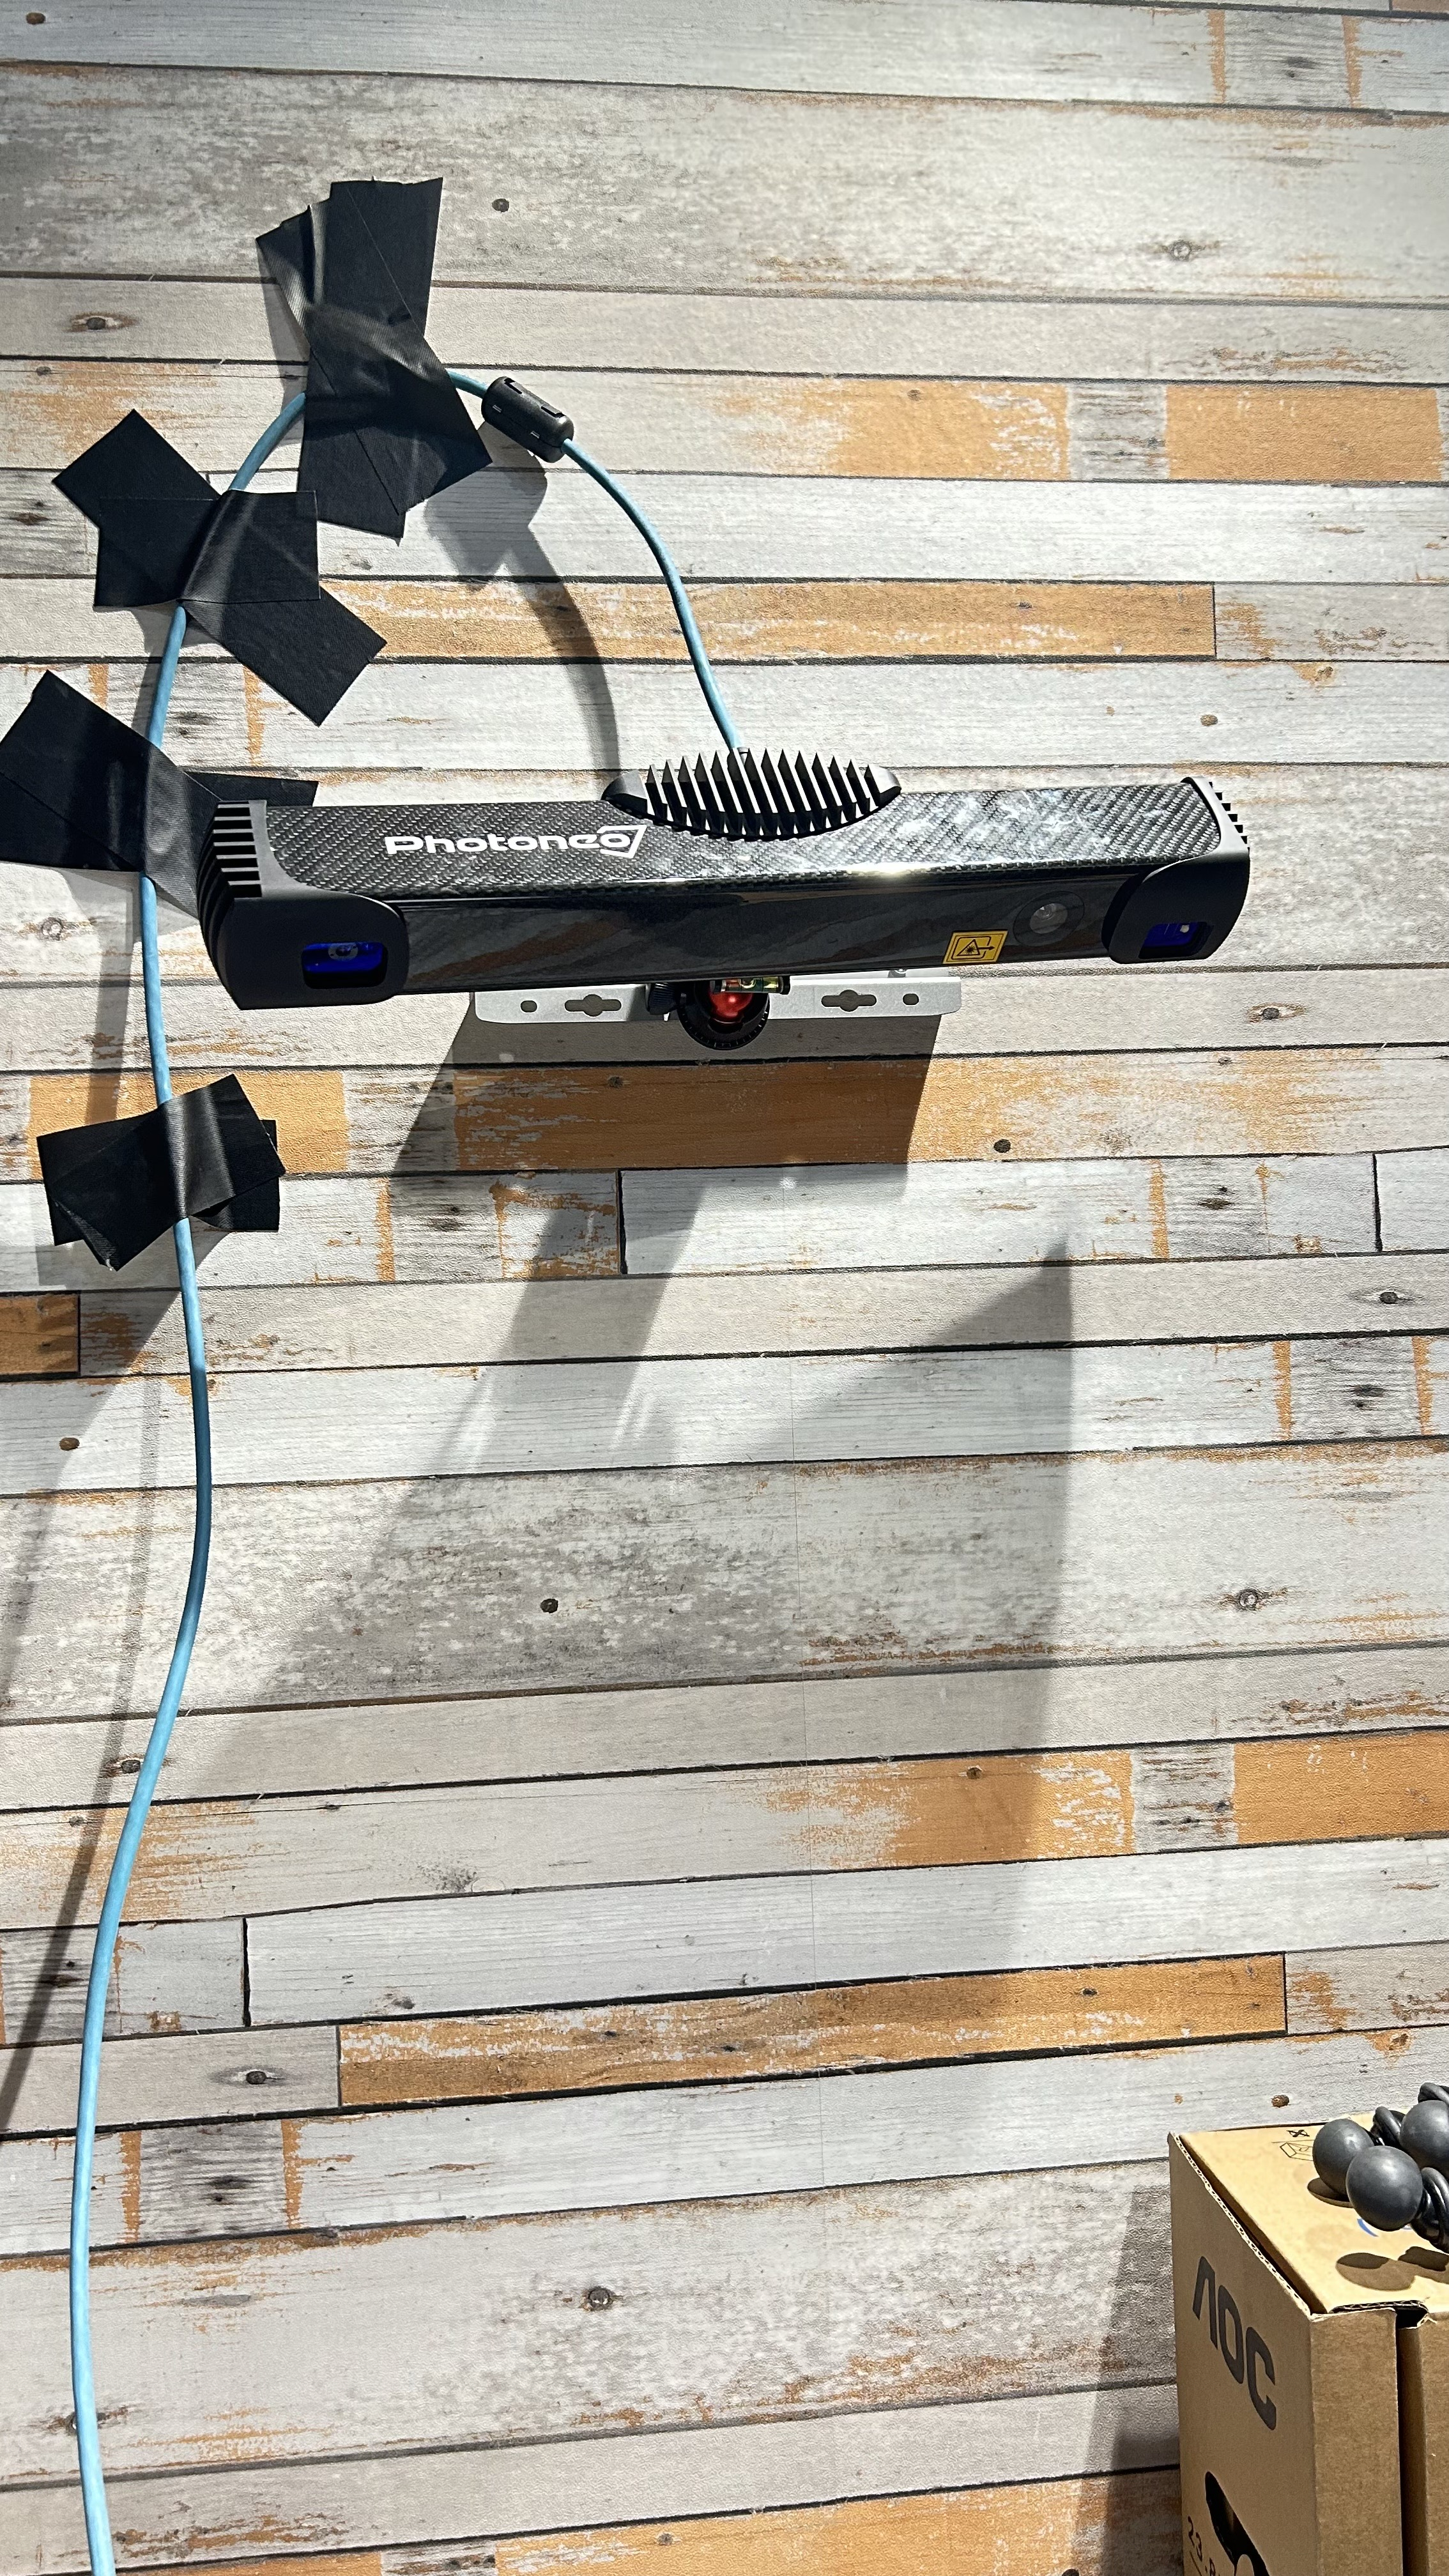
\includegraphics[width=4cm]{Thesis-report/Figures/camera.jpeg}
    \caption{Camera-mounted setup}
    \label{fig:camera-setup}
\end{figure}

The camera is built with a parallel stereo charged-coupled device (CCD) camera system to follow the colored region of the RGB marker accurately. This ROI was also separated from the live stream image using blob analysis, and then the 3D coordinates in the world coordinate frame were triangulated.   The 3D coordinates of the marker were transformed into the robot frame of reference (robot stereo vision coordinate system) and used to evaluate the robot path and trajectory planning.   Consequently, our proposed model determines the real-time distance the robot needs to travel along the three axes to select and position an object\cite{ref15}.

The camera's carbon fiber body is lightweight and guarantees the same degree of stiffness as scanners. Three parts comprise the 3D camera: a camera unit with our proprietary mosaic Shutter CMOS image sensor, a laser projection unit, and a processor unit with a GPU, which is used for intelligent applications.  One well-suited representative of this category is the 3D scanner range from photoneo. This method is appropriate for dynamic scenes because it uses sequential (multi-frame) capturing\cite{ref15}.

\subsection{Position of Camera}
When mounting a camera for vision operation, it is best to keep it stable and as close to the robot's work envelope as feasible, without interfering with or restricting the movement of the robot arm. The longer the part must travel from the camera's location into the robot's reachable workspace, the more errors the encoder counts will produce, since the accuracy of conveyor tracking with vision depends on the coordinate transformation between the camera's picture-taking location and the robot's work envelope. The camera must be oriented downwards since the components are positioned on the conveyor belt's surface, and vision recognition is done on the parts' upper surface. For the camera's 25 mm lens to cover the entire visible portion of the conveyor belt, a camera fixture was constructed to hold the camera directly above the upstream sensor. The upstream sensor is also used to activate the camera to take a photo when parts are presented at this point, so the picture-taking location is placed at the top of the upstream sensor. Following their placement in fixed locations, the camera and conveyor must be calibrated using the calibration program on the robot controller to configure the camera's properties and determine how the locations of the camera and conveyor relate to the robot's world coordinate \cite{ref19}.\

\subsection{Object Identification}
\begin{figure}[h]
    \centering
    \includegraphics[width=8cm]{Thesis-report/Figures/Trapezoid web.jpeg}
    \caption{Object Identification in Web Interface}
    \label{fig:web_interface}
\end{figure}


The STL file is uploaded to the web interface, thereby helping the camera to identify object in the moving conveyor belt tracking system. Once the object is detected, the camera helps in getting the object's position and its quaternion values.

\subsection{Photoneo Camera-Web Interface}

For running the Solution request, after verifying that the environment complies with all necessary safety rules, Button Deploy launches the solution \cite{ref2}.\\

\begin{figure}[h]
    \centering
    
\includegraphics[width=10cm]{Thesis-report/Figures/deploy.jpg}
    \caption{Solution Deployment\cite{ref2}} 
    \label{fig:solution-deployment}
\end{figure}
    
After a defined solution is deployed, runtime requests from action clients are received and carried out.  The user can check the connection statuses of the photoneo 3D Sensors (vision systems) and Action Request Client (robot core software).  It can also stop or resume the deployed solution, as well as call a scan request and a get object request \cite{ref2}.
The deployment page displays a visualizer that displays the following data in addition to console logs that detail earlier events and actions. Real-time visualization of the captured 3D point cloud. Localized objects are displayed with colors that reflect their current state \cite{ref2}.

\begin{enumerate}
    \item Localized \colorbox{green}\\ 
    \item Being picked \colorbox{blue}\\
    \item Rejected \colorbox{red}\\
\end{enumerate}

An inspector tool for each localized object's diagnostics\cite{ref2}

The web interface shows the image of the object being detected; initially, we load the STL file of the object to be captured by the robot. The red color indicates the object, and once the object turns green, the object coordinate will be indicated as quaternion values. After getting the quaternion values, these are transferred to the robotic controller, which helps the robot to reach the desired target position \cite{ref2}.

\begin{figure}[h]
    \centering
    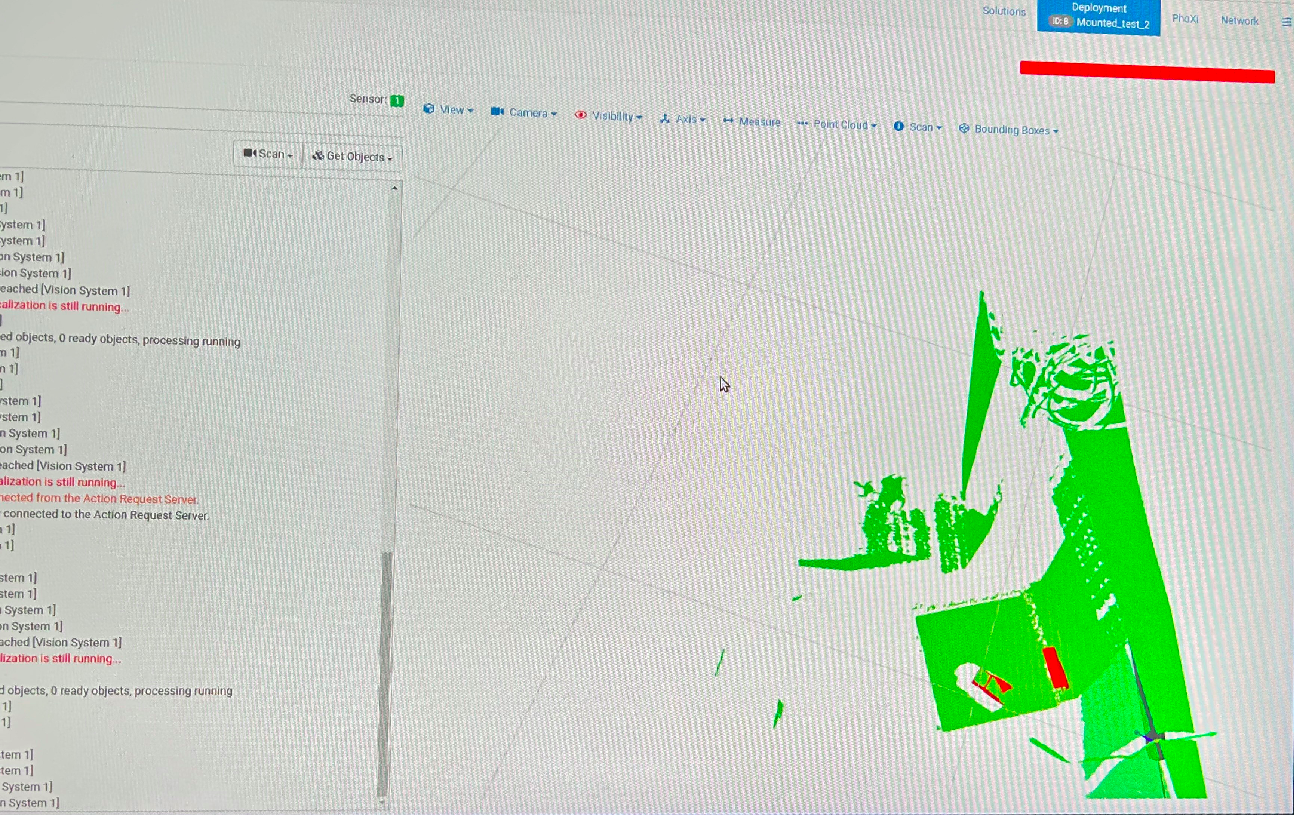
\includegraphics[width=9cm]{Thesis-report/Figures/web_interface.png} 
    \caption{Camera web interface}
    \label{fig:web-interface}
\end{figure}

\begin{figure}[h]
    \centering
    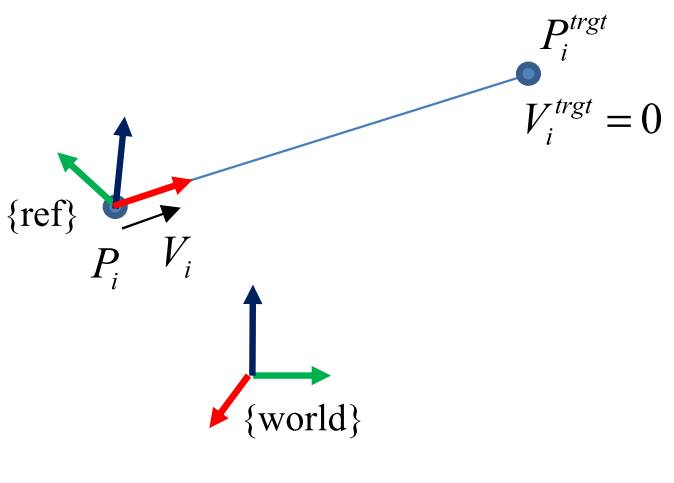
\includegraphics[width=9cm]{Thesis-report/Figures/new.jpeg}
    \caption{Object detection with pipe }
    \label{fig:object-det-with-pipe}
\end{figure}

 The \autoref{fig:object-det-with-pipe}represents the web interface that includes the camera triggering the object placed in the workspace.The red region is the thing that the robot is supposed to pick up, and the green section is the workspace. Using a TCP/IP client, request a connection in which the robot and camera connections are being established. For setting up the connection, the robotic controller and camera IP address (subnet) are made into the same, which helps in communication through a web interface.
 
\begin{figure}[h]
  \centering
  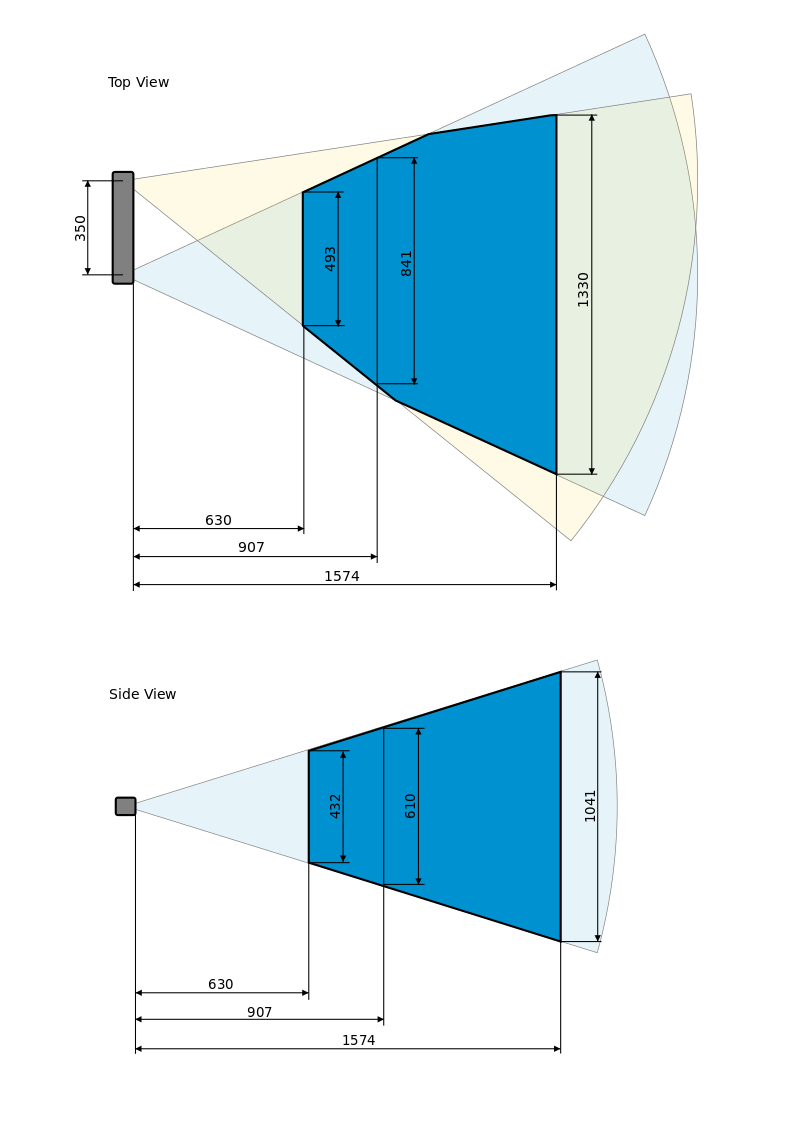
\includegraphics[width=8cm]{Thesis-report/Figures/scanning volume.png}
  \caption{Scanning Volume \cite{ref18}}
  \label{fig:photoneo-scanning-volume}
\end{figure}

The \autoref{fig:photoneo-scanning-volume} shows the volume/area in which the photoneo Camera can scan items and determine object poses. The top view shows the maximum field of view (FOV) reachable by the camera for object coordinate acquisition, which extends up to 15 m. The camera sits around 350 mm tall and projects a pyramidal field of view with colored ones. The Depth lanes at 630 mm, 907 mm, and 1574 mm from the sensor; at each distance, the intersection of the FOV with the flat plane is a rectangle that grows with distance. moreover, the blue trapezoid is the maximum rectangular cross-section of the scan volume with sensor horizontal, vertical, and diagonal field of view limits \cite{ref2}.


\subsection{Calibration for camera}

For camera calibration, the following steps need to be followed and considered: \cite{ref2}
\begin{enumerate}
    \item  ID: the Vision system's ID \cite{ref2}
    \item  Name: the Vision system's name \cite{ref2}
    \item  Scanner ID: the 3D sensor's ID that the vision system uses \cite{ref2}
    \item  Scanner status: the current state of the 3D sensor used by the Vision system\cite{ref2}
    \item  Scanner model: the 3D sensor model that the vision system uses \cite{ref2}
    \item  Calibration type: the type of calibration based on the selected 3D sensor mount position \cite{ref2}
    \item  Calibrated: whether the Vision system has already been calibrated \cite{ref2}
    \item  Accuracy of calibration [mm]: the precision of any prior calibration   \cite{ref2}
\end{enumerate}

\begin{figure}[h]
    \centering
    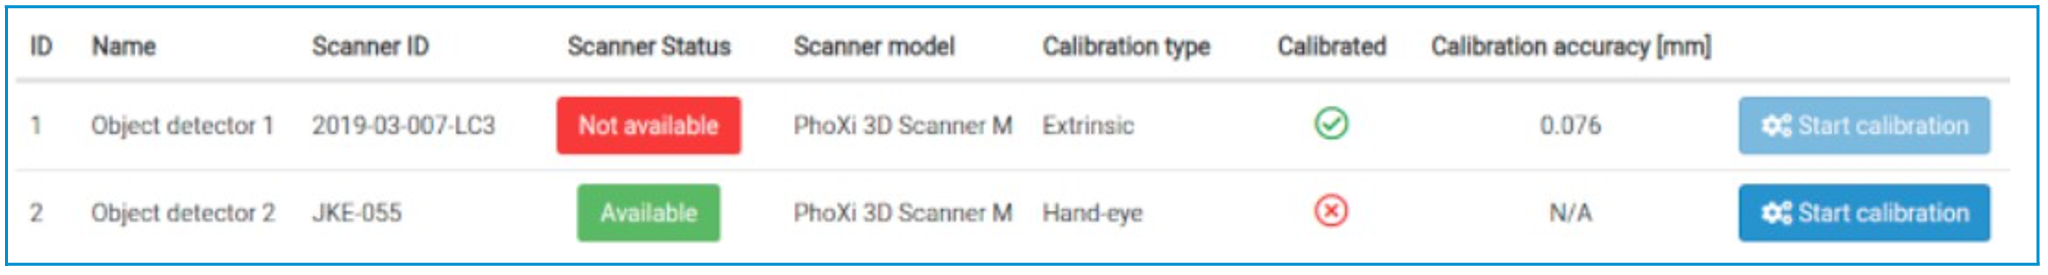
\includegraphics[width=13.5cm]{Thesis-report/Figures/calib.png}
    \caption{Calibration \cite{ref2} }
    \label{fig:Photoneo Cmaera}
\end{figure}
The camera is set in place, and the calibration ball is fixed at the end of the robot's Tool Center point as part of an extrinsic method for camera calibration.\\
\begin{figure}[h]
    \centering
    \includegraphics[width=12cm]{Thesis-report/Figures/calibration.jpeg}
    \caption{Calibration for camera relative to the robot frame\cite{ref2}} 
    \label{fig:Photoneo Cmaera}
\end{figure}
Figure 37 below shows how the calibration is happening by adding the point by fixing the point where the robot coordinates [X, Y, Z] rotation values will save the points (represented as a green point). Here, we need to add 9 points to get the calibration workspace. After the calibration, the average value from the 9 points is taken into consideration. (The lesser the value, the better the accuracy) \cite{ref2}.\\ 

The calibration method employed in this study (extrinsic calibration) (EC) is depicted in Figure 38 below. The camera is fixed in the site, and nine points are considered before the average value is ultimately chosen as the calibration value.  [2]  In configurations where the 3D sensor is fixedly positioned within the robotic cell, frequently above the bin, this type of calibration is used.  The 3D sensor just needs to be stationary concerning the robot's base; it is not required to be stationary concerning the robotic cell itself.  [2]  Finding a camera's intrinsic matrix, extrinsic matrix, and distortion coefficients is the aim of camera calibration \cite{ref2}.\\ 

\begin{figure}[h]
    \centering
    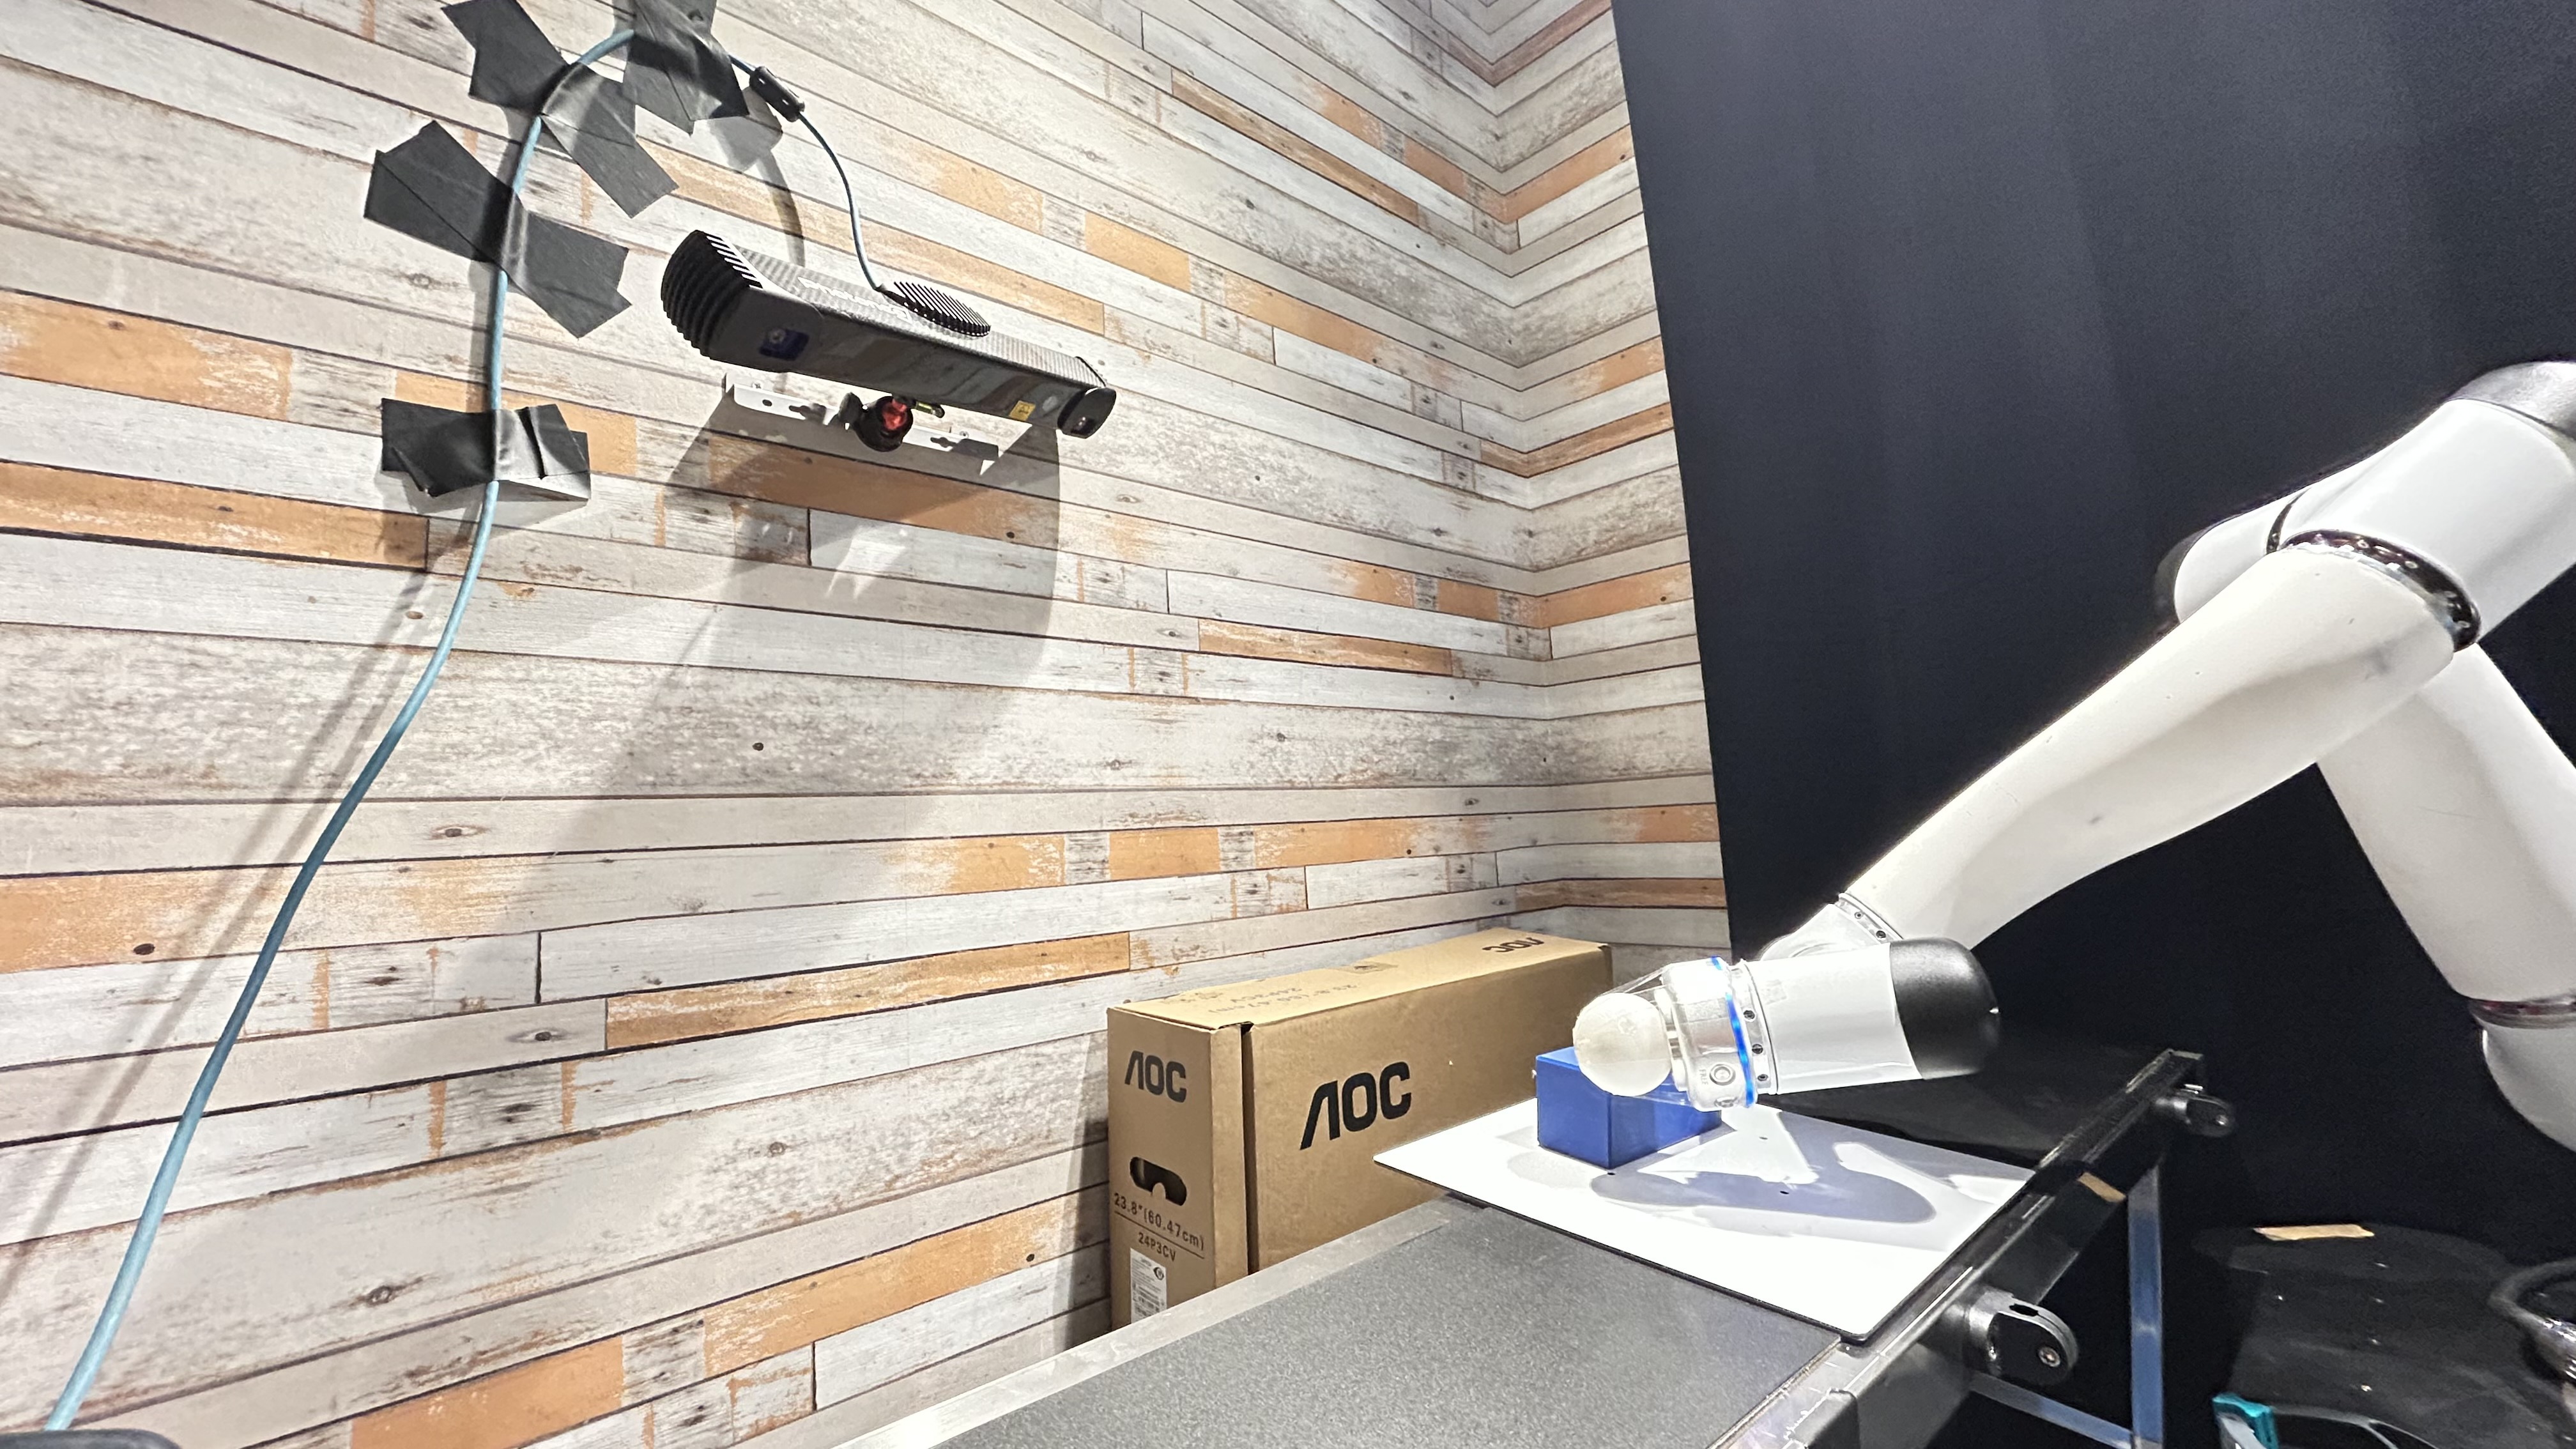
\includegraphics[width=10cm]{Thesis-report/Figures/extrinsic_ball.jpeg}
    \caption{Calibration for the camera relative to the Robot frame}
    \label{fig:Photoneo Cmaera}
\end{figure}
The intrinsic matrix describes the relationship between the picture plane and the camera frame, while the extrinsic matrix describes the relationship between the camera frame and the chessboard frame.  Establishing the transformation relationship between the cameras and the robotic arm is the goal of hand-eye calibration.  Once the transformation link is established, the location of an object in the camera frame may be translated into its location in the robot base frame. The robotic arm will then be able to locate the object and pick it up. Finding the transformation matrix between the robot base and the camera (base H cam) is the aim of an eye-to-hand calibration \cite{ref3}. The equation below is taken from \cite{ref3}.\\

 \[
{}^{\text{cam}}\mathbf{H}_{\text{cal}} = {}^{\text{cam}}\mathbf{H}_{\text{base}} \cdot {}^{\text{base}}\mathbf{H}_{\text{tcp}} \cdot {}^{\text{tcp}}\mathbf{H}_{\text{cal}} = {}^{\text{cam}}\mathbf{H}_{\text{base}} \cdot {}^{\text{base}}\mathbf{H}_{\text{cal}} \tag{3}
\]


The transformation matrix in the equation above that must be computed for the eye-to-hand calibration is the camera H base, or the position of the robot's base frame, as shown in the camera frame. Additionally, the Cam H cal is the transformation matrix from the calibration rig frame to the camera frame and can be calculated using either 3D recognition of the calibration rig or camera calibration (extrinsic matrix)  Base H cal, or the pose of the calibration object's frame cal expressed in the robot's base frame, can be computed using forward kinematics. This is usually accomplished by identifying the calibration target from a known robot pose. The matrix of mathematical transformations between the calibration rig frame and the robot base frame. The calibration matrix will be considered invalid, and the entire calibration process will need to be restarted if the relative positions of the robot and the 3D sensor change after the calibration.  In other words, after the system has been calibrated, the 3D sensor cannot be moved around the robot \cite{ref3}.\\


\begin{figure}[h]
    \centering
    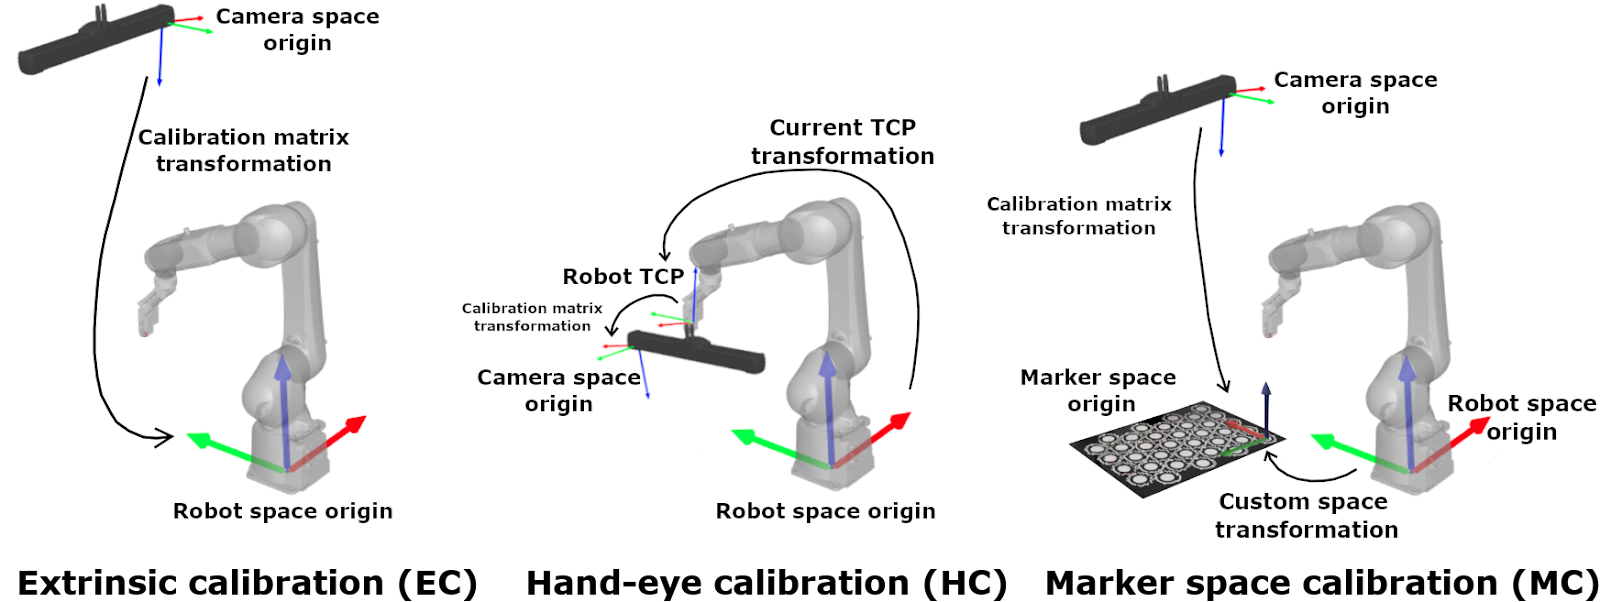
\includegraphics[width=13cm]{Thesis-report/Figures/extrinsic.png}
    \caption{Extrinsic Calibration \cite{ref2} } 
    \label{fig:Photoneo Cmaera}
\end{figure}

The calibration matrix specifies the transformation straight to the robot base coordinate system because the 3D sensor is fixed. With this configuration, the robot's mobility is unrestricted, and it doesn't need to halt during the scan acquisition, unlike with the hand-eye approach\cite{ref2}.
\subsection{Static picking}
\begin{figure}[h]
    \centering
    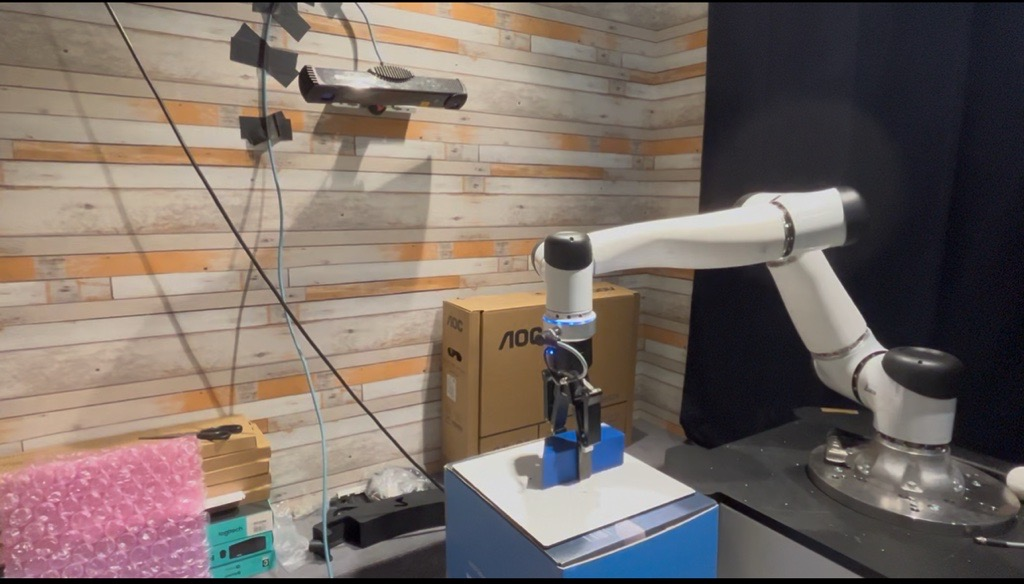
\includegraphics[width=10cm]{Thesis-report/Figures/static.jpeg}
    \caption{Static picking}
    \label{fig:Photoneo Cmaera}
\end{figure}

Static pick-up is the process of picking items from the conveyor belt when it is not moving. Initially, we keep the object on the conveyor belt and then trigger the camera, which helps in getting the object coordinates to the robotic controller. When the robot receives the data, the robot moves to the target position to pick the required target.

\begin{figure}[h]
    \centering
    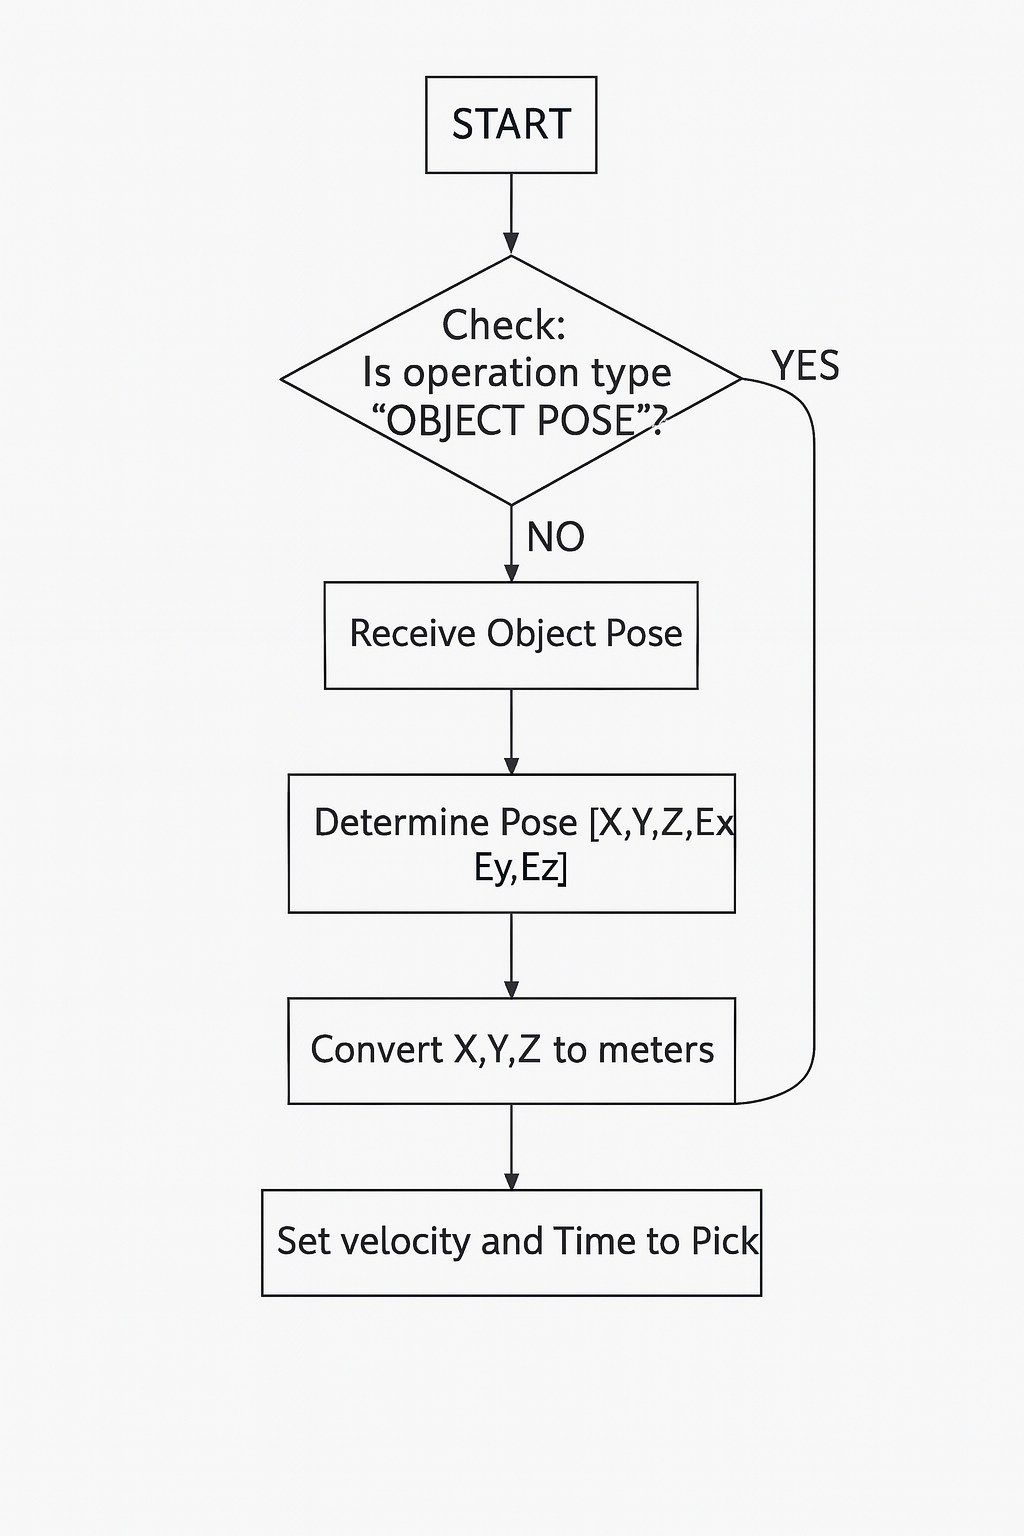
\includegraphics[width=6.5cm]{Thesis-report/Figures/static_flowchart.png}
    \caption{Static picking Flowchart}
    \label{fig:Photoneo Cmaera}
\end{figure}


\subsection{Dynamic picking}
The Dynamic pick involves the process of picking the items from the moving conveyor belt. Here, the object is passed through the moving conveyor belt, where the camera gets object poses that are passed to the robotic controller, which helps the robot move to the required position.\\
\begin{figure}[h]
  \centering
  \begin{minipage}{0.45\textwidth}
    \centering
    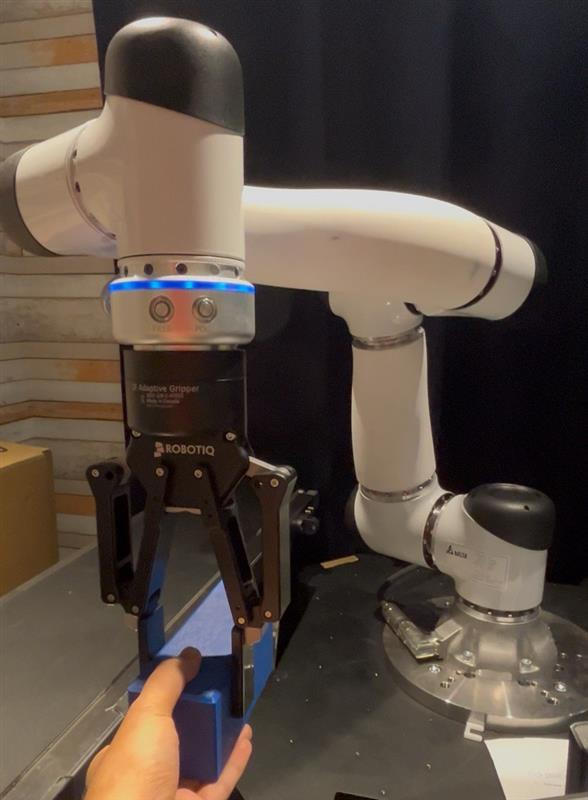
\includegraphics[width=4cm]{Thesis-report/Figures/pick.jpeg}

  \end{minipage}%
  \hspace{5mm}% ← adjust this (or make it negative: e.g. \hspace{-3mm})
  \begin{minipage}{0.45\textwidth}
    \centering
    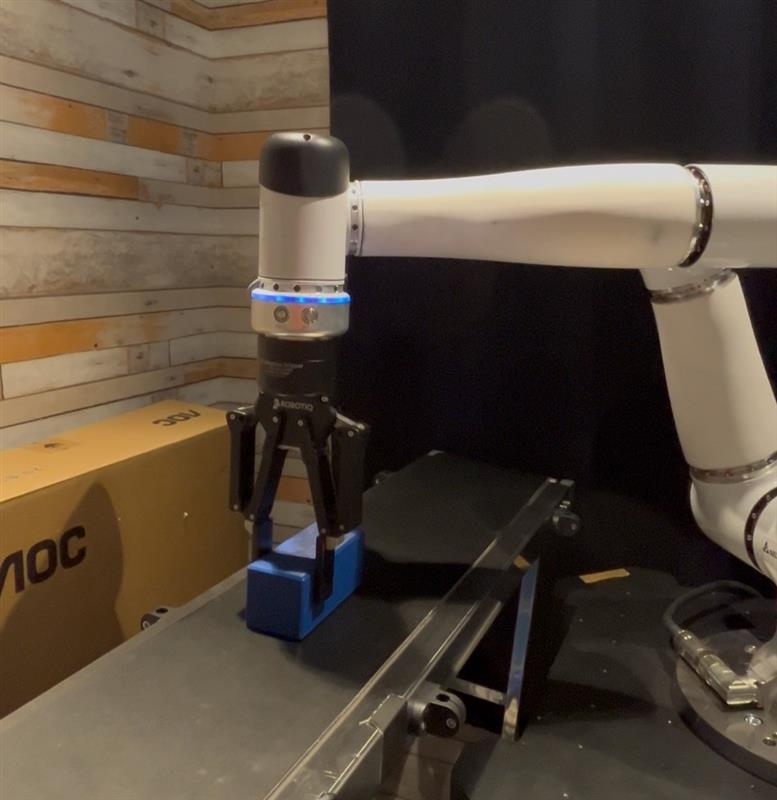
\includegraphics[width=5cm]{Thesis-report/Figures/picking.jpeg}

  \end{minipage}
  \caption{Dynamic picking}
  \label{fig:gripper-combined}
\end{figure}

For dynamic picking, a typical construction site is needed, and quick, real-time modeling is necessary to support decision-making.  Thus, a quick 3D data collection and processing system is required for real-time modeling of a building site.  Only high-quality, rich 3D datasets of static objects are produced using laser scanners; a typical scan has millions of points.  Furthermore, real-time modeling is not practicable due to the slowness of data collection and processing.  Nevertheless, 3D range cameras provide an additional option by enabling wide-field-of-view, low-cost, automatic tracking and detection of both static and moving objects at frame rates higher than 1 Hz in real-time.\\

The dynamic movement can be explained as follows:

Initially, we pass the object through the running conveyor belt and trigger the camera, where we get the initial and final coordinates. We also calculate the timestamps to get the changes in time. The custom velocity must then be determined, which can be done by dividing the position change by the time change.
When we pass the object through the conveyor belt, there is a change in position in the X axis, as this is a linear motion of movement. For the robot to know where to go and get the item from the conveyor belt, it must be notified when the object's position changes.  The following formula can be used to adjust for this:: $X = X_0 + v\cdot t$ where $X_o$ where $X$ is the object's starting position.\\
where X represents the object's starting position\\
X represents its ending position.\\
t is the change in time. 


\subsubsection{Calibration Ball}
A calibration ball serves as the calibration object. It is also possible to replace the calibration ball with a specially designed ball that has the proper properties; the ball must be precisely round and made of a surface that is suitable for scanning (smooth and not very reflective). The ball needs to be attached to the gripper or the flange, which are the robot's endpoints. During the calibration process, make sure the ball is securely attached and stays in place. Verify that the ball can be seen clearly by the 3D sensor\cite{ref2}. \\
\begin{figure}[h]
    \centering
    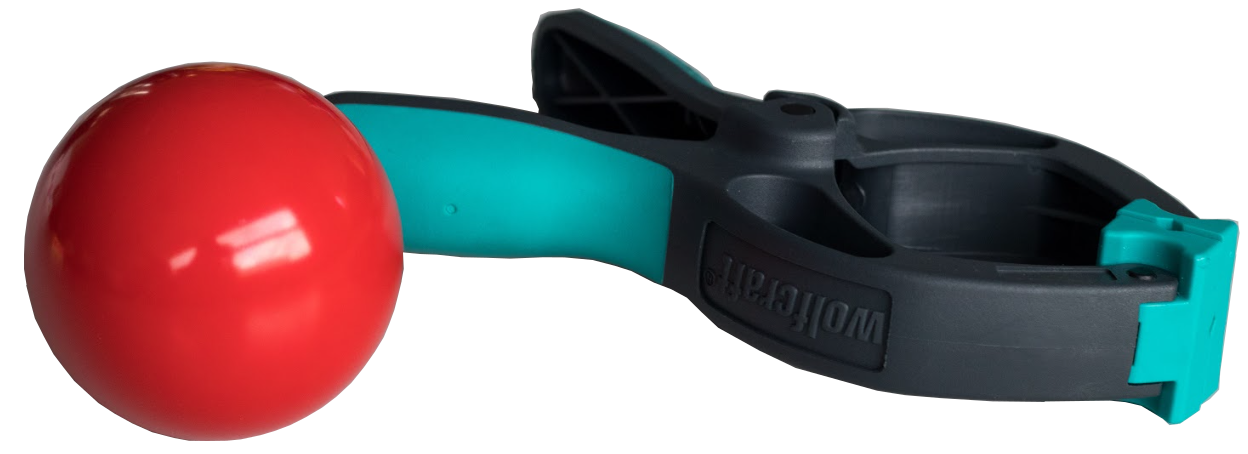
\includegraphics[width=3cm]{Thesis-report/Figures/ball.png}
    \caption{Calibration ball \cite{ref2}}
    \label{fig:Photoneo Cmaera}
\end{figure} 


The following components make up the calibration interface:
\begin{enumerate}
    \item   Visualization: The Verification and Texture tabs can be switched between.
 (Texture tab) Texture image. The texture image was created by the most recent scan acquisition. If the localized calibration ball was successfully located for the extrinsic calibration, it is indicated with a green highlight. However, that portion of the texture will be highlighted in red if there is not enough ball surface visible or if another item with a similar form is found \cite{ref2}.
 \item   3D visualizer (Verification tab) 
The visualizer shows the point cloud and 3D sensors from all vision systems.
 After adding the required number of calibration points, the following items show up: \cite{ref2}
\item  Add calibration point: a button to begin a fresh scan, usually to get the most recent point cloud for validation \cite{ref2}
\begin{figure}[h]
    \centering
    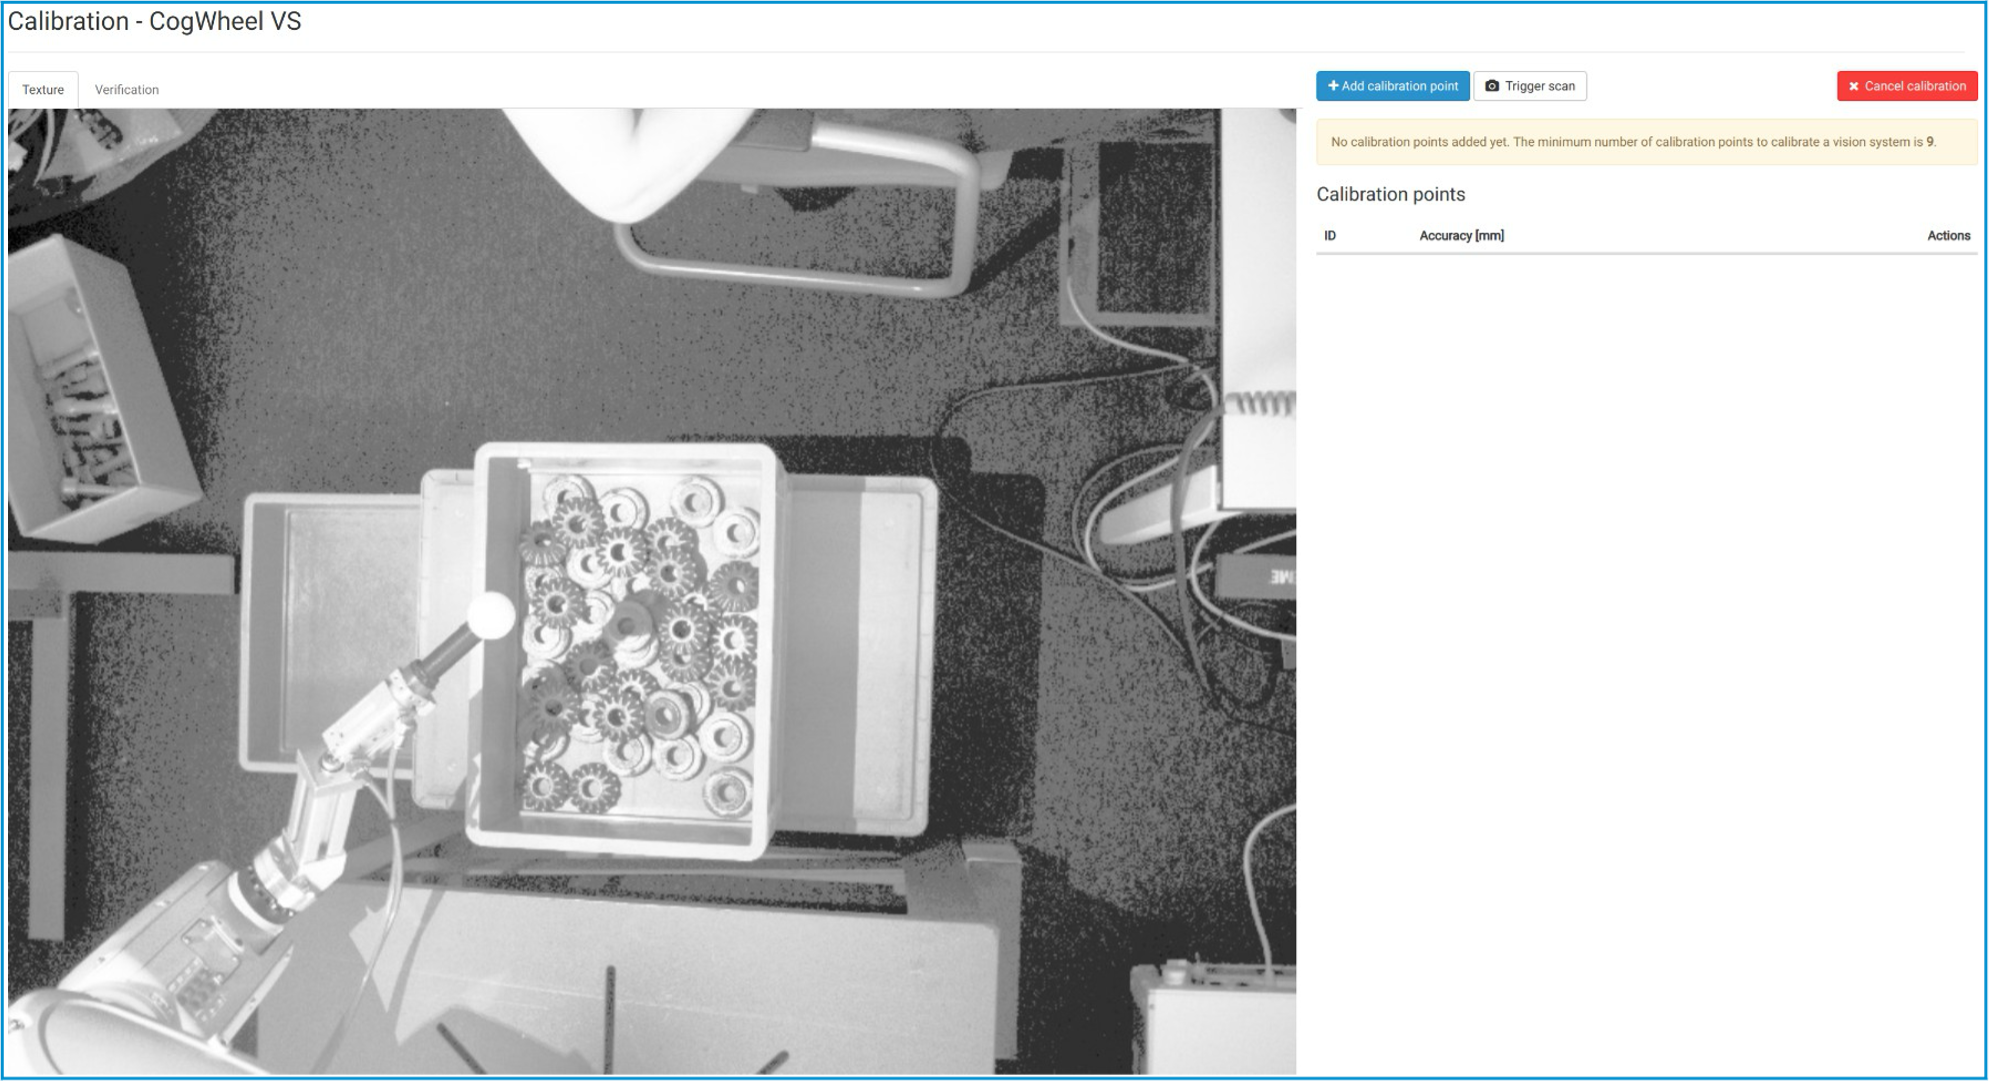
\includegraphics[width=12cm]{Thesis-report/Figures/calibration_procedure.png}
    \caption{Calibration using the calibration ball \cite{ref2} }
    \label{fig:Photoneo Cmaera}
\end{figure} 

\item   Trigger scan: a button for starting a new scan, typically used to obtain the current point cloud for verification purposes \cite{ref2}
\item  List of calibration points: an inventory of all calibration points that have been successfully inserted, together with each point's accuracy and deletion option. The outcome of the calibration process is the calibration matrix\cite{ref2}.
\item   Accuracy of calibration: overall calibration accuracy \cite{ref2}.
\item  To finish the calibration procedure and save the calibration matrix result into the vision system, press the "Finish and save result" button\cite{ref2}.
\end{enumerate}

The 3D sensor must record the calibration ball in several locations throughout the entire region of interest during the extrinsic calibration process. Similarly, during the hand-eye calibration, the marker plate must be captured by the 3D sensor from various angles.  Therefore, by adding a new calibration point, the robot can move in a range of configurations with as many distinct joint orientations as feasible in each position \cite{ref2}.

Either a new calibration point is introduced:
\begin{enumerate}
    \item The Add calibration point button in the calibration web interface can be manually pressed by the operator\cite{ref2}.
    \item The robot can call the Add calibration point request \cite{ref2}.
\end{enumerate}

After starting the scan acquisition, a new calibration point is added to detect the calibration tool (ball or pattern).  A flash message alerting the user to the successful outcome appears if the detection is successful. If the calibration point is not inserted, a permanent error notice 65 will display, explaining the cause of the fault and how to correct it \cite{ref2}.

\begin{figure}[h]
    \centering
    \includegraphics[width=12cm]{Thesis-report/Figures/point.png}
    \caption{Calibration point saved \cite{ref2}}
    \label{fig:Photoneo Cmaera}
\end{figure} 

Three calibration sites are needed for both the hand-eye and extrinsic calibration. The resulting calibration matrix and the calibration accuracy information are only accessible after the required number of calibration points has been added \cite{ref2}.\\
 
 Location of point clouds and 3D sensors: When the fourth point is added during extrinsic calibration and the fifth point is added during hand-eye calibration, the model of the 3D sensor of the currently calibrated vision system starts to mirror the pose of the real 3D sensor.  At the same time, the point cloud is displayed \cite{ref2}.\\
 Every calibration point that has been successfully inserted has an ID and a unique accuracy score that is measured in millimeters.  The confidence level in correctness increases as the accuracy score decreases.  The Delete option can be used to eliminate a point from the dataset if its accuracy score is excessively high \cite{ref2}.

\subsection{Extrinsic Calibration Results}
\begin{table}[h!]
\centering


\label{tab:transformation_matrix}
\scalebox{1.3}{
\begin{tabular}{|c|c|c|c|}
\hline
-0.327147 & -0.736148 & 0.592503 & -1171.593426 \\
\hline
-0.944628 & 0.271707 & -0.183991 & -234.525444 \\
\hline
-0.025543 & -0.619888 & -0.784275 & 685.496959 \\
\hline
0.000000 & 0.000000 & 0.000000 & 1.000000 \\
\hline
\end{tabular}
}
\caption{Calibration Results}
\end{table}

 The total calibration accuracy score, reported in millimeters, is a measure of calibration quality.  Attempt to score the lowest possible score at all times.  Numerous elements, including optic arm size, calibration ball quality,eters, lighting conditions, and conditions, and impact on the value. The calibration accuracy value is used to confirm the calibration's quality . Furthermore, the approximate accuracy of the output (without taking precision into account) can be confirmed by evaluating the position of the 3D sensor and the point cloud in the image.
 The coordinate frame of the robotic controller used for the calibration procedure contains the scene's origin. Usually, that alludes to the robot base's origin.  The relative positions of the scene origin and the 3D sensor model should then coincide or match those of the robot base and the actual 3D sensor.

 \subsection{Conditions for Conveyor Belt}
While setting up the conveyor belt with a vision camera, we need to follow certain conditions:

1. \textbf{Matching the robot speed with the conveyor belt} For the robot to pick up the object from the conveyor belt, the robot's end effector should move at the same speed as that of the conveyor belt \cite{ref21}.

The below eqautions are taken from : \cite{ref21}
\[
V_c = V_r 
\]

where \( V_c \) represents the velocity of the conveyor belt and \( V_r \) represents the velocity of the robot\cite{ref21}.\\

2. \textbf{Target position Calculation} The final position of the robot is calculated by:

\[
\text{Target} = TX + AMS \cdot \theta + TD 
\]

\text{where } TX \text{ is the initial detected position, } AMS \text{ is the marker space displacement, and } TD \text{ is the tracked distance}\cite{ref21}.\\


3. \textbf{Marker Space Displacement (AMS()} \\

\[
AMS \cdot \theta = TX - \text{MPO}
\]

 where mPO is the marker pattern Origin, $TX$ the initial detected position, $AMS$ helps in getting the relative position to this reference, and the marker pattern Origin is the reference\cite{ref21}.

4. \textbf{Tracked Distance} 

\[
TD = \Delta TSC + \Delta CTO 
\]

\begin{itemize}
  \item $\Delta TSC$ is the \textbf{Target Scan Completion Distance}%
        —Distance moved by the conveyor during scan completion\cite{ref21}.
  \item $\Delta CTO$ is the \textbf{Conveyor Tracking Offset}%
        —Conveyor tracking offset, or $\Delta CTO$, is the distance traveled while awaiting the robot to arrive at the pick place\cite{ref21}.
\end{itemize}

5. \textbf{Target Scan Completion Distance (TSC)} 

\begin{center}
    \[
    TSC = V_c \times t_s 
    \]
\end{center}

6. \textbf{Final Adjusted position}\\

After considering the conveyor motion and processing delays, the final position will be the place where the robot should pick the object \cite{ref21}.\\

\[
\text{Target} = TX + (TX - \text{MPO}) + (V_c \times t_s) + (V_c \times t_r)\
\]

where mPO=Marker pattern Origin
\subsubsection{Calibration of Conveyor Belt}
The following methods can be used to calibrate the conveyor belt:  The inputs and outputs are shown in the below \autoref{fig:conveyor_belt with cmaera}. The inputs include:

\begin{figure}[h]
    \centering
    \includegraphics[width=13cm]{Thesis-report/Figures/conveyor_belt with cmaera.jpg} 
    \caption{Conveyor tracking setup}
    \label{fig:conveyor_belt with cmaera}
\end{figure}

\begin{itemize}
\item \textbf{Scan request}\\
The scan request consists of a  python code that is used to send a request to the camera, which is then taken by the vision controller or the vision control box that helps trigger the camera \cite{ref21}.
 \item \textbf{Trigger scan}\\
 The trigger scan can be of the SW or HW method, where the output is hardware or software \cite{ref21}.

\item \textbf{Trigger }\\
Initially, the scan request is given to the vision controller, creating a trigger scan that helps the camera trigger\cite{ref21}.
The output section includes the following:
\end{itemize}

\begin{itemize}
\item \textbf{Coordinates of localized object}\\
The coordinates of the localized object consist of the object [X, Y, Z, Rx, Ry, Rz, and W], where X, Y and Z include the coordinates of the object and [Rx, Ry, Rz, and W] include the quaternion values (rotation values), which are identified by the vision camera \cite{ref21}.

\item \textbf{ Scan}\\
Once the trigger commands reach the camera, the scan will start to take place and take the objects as mentioned above \cite{ref21}.
\item \textbf{Final position} \\ 
The final position is considered the location where the object coordinates, along with the calibration offset and traveled distance \cite{ref21}.
\end{itemize}

\begin{enumerate}
\item {Calculate the pick pose} \\
We must first ascertain the location of the object that needs to be raised \cite{ref21}.

\item {Components of the pick pose calculation}
 Coordinates from localization in marker space (calculate the transformation matrix from camera space to marker space to calibrate the marker pattern)\cite{ref21}

\end{enumerate}
Possible triggers for the distance traveled from acquisition to the beginning of picking in conveyor tracking mode include\\

The scan request function pho wait for req completion() in SW-HW output of the trigger \\

\begin{enumerate}
\item{Calibration Distance:}
The distance between the marker pattern positions for the camera calibration and custom workspace calibration (the linear transformation between the camera and the custom WS origin) is known as the calibration distance\cite{ref21}.\\
\end{enumerate}

\begin{figure}[h]
    \centering
    \includegraphics[width=13cm]{Thesis-report/Figures/conveyor_belt.jpg} 
    \caption{Conveyor Belt setup \cite{ref21}}
    \label{fig:Photoneo Cmaera}
\end{figure}
Figure 47 above depicts the calibration board, which is used to ascertain the object's X, Y, and Z coordinates in conjunction with the conveyor belt.The target position is T[X, Y, Z, Rx, Ry, Rz], which represents the quaternion value of the object that needs to be converted into Euler values that are used to move the robot to that specified location. mSD stands for marker space displacement, TD for travel distance, and TSC for trigger to scan completion in meters \cite{ref21}. \\


In Figure 48 below, the number represents the coordinates of the object after the scanning of the object is done, after the trigger. Once these quaternion values are attained, these values are then sent to the robotic controller for the robot to move to the required target position.\\\\
\begin{figure}[h]
    \centering
    \includegraphics[width=13cm]{Thesis-report/Figures/coordinates.png} 
    \caption{Coordinates of object}
    \label{fig1.Photoneo Cmaera}
\end{figure}

Calibration of the marker pattern from the camera to the conveyor belt, which is the common origin:
\begin{enumerate}
    \item Attach the appropriate calibration pattern to the conveyor belt \cite{ref21}.
    \item Use phoXi Control's marker pattern to save calibration. We can use this setting as a custom scanning mirror in Vision System's Space by adding a triggering item for the sensor at the marker pattern export photo's origin \cite{ref21}.
    \item Robot to conveyor belt: The robot moves the conveyor belt from a shared origin, but the marker pattern stays in place according to the conveyor belt. This allows the robot to reach the marker pattern, calibrate the custom coordinate space in the robot track, and save the "calibration" encoder value, which synchronizes the robot and conveyor\cite{ref21}. 
\end{enumerate}

\subsection{Manual Calibration}
Initially, before we start the calibration, we need to set the camera to a specific mrile setup to marker Space according to the calibration setup and save the mrile as given below: \cite{ref2}

\begin{figure}[h]
    \centering
    \includegraphics[width=13cm]{Thesis-report/Figures/manual.png} 
    \caption{Manual calibration \cite{ref2} }
    \label{fig1.Photoneo Cmaera}
\end{figure}


The conveyor belt can also be calibrated using this technique.  Among the steps are:
\begin{enumerate}
    \item \textbf{First step:}  First, position the picking/triggering object in the camera's field of view, then press the trigger to obtain the object pose, which consists of [X1, Y1, and Z1] in that order\cite{ref2}.
    \item \textbf{Second step:} Switch on the conveyor belt and get the farthest position where the camera triggers the object, and get the coordinates, which include [X2, Y2, and Z3] respectively\cite{ref2}.
    \item \textbf{Third step:}In addition to triggering the camera in the initial and final positions, we attempt to record the camera's timestamps, which determine how long it takes the camera to trigger\cite{ref2}.
    \item \textbf{Fourth step:} The fourth stage involves calculating the change in position for \(X\), \(Y\), and \(Z\), respectively. This comprises calculating \((\Delta X, \Delta Y, \Delta Z)\). Furthermore, we must obtain the change in time \(\Delta t\)\cite{ref2}.
    \item \textbf{Sixth step:} In order to obtain a change in position as linear motion and transmit it to the robotic controller that assists the robot in picking up items from the conveyor belt, we must lastly multiply the custom velocity by the time and position changes along the X position\cite{ref2}.
\end{enumerate}



\subsubsection{Encoder offset}
Types and Technologies of Encoders
Although encoders come in a wide variety of forms, they essentially fall into two primary sensing categories. These include:

\begin{enumerate}
    \item  Linear
    \item Rotating/Rotational
    
\end{enumerate}

There are various encoder measuring types within those categories, including
\begin{enumerate}
    \item Complete
    \item Gradual
\end{enumerate}
Additionally, there are several electromechanical technologies, including
\begin{enumerate}
    \item magnetism
    \item Optical
    \item Inductive
    \item Capacitive
    \item Laser 
\end{enumerate}

The controller receives counts as the encoder rotates. Assume that the count range is between 0 and 10,000. Since this is an incremental encoder, we know that a full rotation of the shaft records a count of 10,000, but we do not know the exact location. When the entrance photo-eye sensor recognizes the object after it has been placed on the conveyor, the current encoder count will be noted. Assume that $5232$ is the number\cite{ref27}.

The below equation are taken from: \cite{ref27}
\[
C_{\text{in}} = 5232 \quad \text{(encoder count at entry)}
\]
\[
C_{\text{out}} = 6311 \quad \text{(encoder count at exit)}
\]
\[
N = 10{,}000 \quad \text{(total counts per revolution)} 
\]

To compute the encoder count difference (accounting for potential wrap-around):

\[
\Delta C = (C_{\text{out}} - C_{\text{in}} + N) \mod N 
\]
\[
\Delta C = (6311 - 5232 + 10{,}000) \mod 10{,}000 = 1079 
\]

The fraction of a full revolution is:

\[
L_{\text{rev}} = \frac{\Delta C}{N} = \frac{1079}{10{,}000} 
\]

The corresponding angular displacement is:

\[
\Delta \theta = L_{\text{rev}} \times 360^\circ = \frac{1079}{10{,}000} \times 360^\circ = 38.844^\circ 
\]

\noindent
Therefore, the object moved a distance equivalent to 1079 encoder counts, or approximately $38.844^\circ$ of the encoder shaft's rotation, between the entry and exit sensors\cite{ref27}.\\

After the object leaves and is picked up by the exit photo-eye, we record $C_{\mathrm{out}}=6311$.  Deducting $C_{\mathrm{in}}=5232$ gives $\Delta C=1079$ counts.  This tells us the object traversed 1079 encoder counts from entrance to exit, though its exact position on the shaft remains unknown.\cite{ref27}.
\subsection*{Linking Encoder Counts to \(v\)}

From your encoder you measured \(\Delta C\) counts over an interval \(\Delta t\). Since one revolution (10\,000 counts) corresponds to moving the belt by one pulley‐circumference \(L_{\mathrm{circ}}\), you get
\[
\text{distance traveled in }\Delta t
\;=\;\frac{\Delta C}{N}\,L_{\mathrm{circ}}
\;\Longrightarrow\;
v
\;=\;\frac{\displaystyle\frac{\Delta C}{N}\,L_{\mathrm{circ}}}{\Delta t}
\;=\;\frac{\Delta C}{N}\,\frac{L_{\mathrm{circ}}}{\Delta t}.
\]
Once you know \(v\), you can predict the object’s future position without waiting for the exit sensor\cite{ref27}.

\subsubsection*{Using \(X = X_0 + v\,t\) for the pick‑and‑Place Robot}

As soon as the entry photo‑eye trips, record
\[
X_0 = 0
\]
(or whatever your belt‑coordinate zero is) and start a timer.

Continuously compute
\[
X(t) = X_0 + v\,t.
\]

When \(X(t)\) reaches the robot’s pickup location, command the robot to grab.

\subsubsection*{Why It’s Helpful}
\begin{itemize}
  \item \textbf{Predictive:} Only time and speed are now required at the pick point, eliminating the need for a second sensor.
  \item \textbf{Smooth motion:} The robot's arm is synchronized with the belt because it may begin moving into position beforehand.

\end{itemize}


\newpage



\newpage
\section{Results and Discussions}
\subsection{Robot TCP Speed vs Conveyor Speed}
The tool-center-point (TCP) speed of the robot is compared to the belt speed.
 The solid blue line indicates the 1:1 identity line, or flawless conveyor tracking, while the red circles plot the average TCP speed over several passes of the robot's end effector.  The robot's average TCP speed increases nearly linearly from 0.08 m/s to 0.31 m/s while the belt speed is scaled from 1.00 m/s to 2.00 m/s, continuously trailing the conveyor by 0.20 to 0.25 m/s.The TCP speed only increases by roughly 0.26 m/s for every 1 m/s increase in belt speed, according to a linear fit (dashed gray) that produces a slope of roughly 0.26 (R2 = 0.995).  When trying to match the belt's high-speed motion, the robot's dynamic limits—inertia, joint acceleration limitations, and control bandwidth—are the main cause of this systematic shortfall.
 
\begin{figure}[h]
    \centering
    \includegraphics[width=11cm]{Thesis-report/Figures/conveyor_speed vs Robot tcp speed.png}
    \caption{Robot TCP speed and Conveyor speed \cite{ref22}}
    \label{fig1.Photoneo Cmaera}
\end{figure}


\subsection{Success Rate vs Conveyor Speed}
Figure 51 compares how effectively our robotic arm picks two shapes—trapezoidal blocks and cylindrical pipes—from a conveyor belt moving between 1.0 m/s and 2.0 m/s. As the belt speeds up, both success rates steadily drop: trapezoid grasps fall from 90 percent at 1.0 m/s to 85 percent at 2.0 m/s, while pipe grasps decline more sharply from 70 percent down to 60 percent. Throughout the range, trapezoids outperform pipes by about 20–25 percentage points, due to their flat faces and edges that give the gripper firm, predictable contact—whereas smooth, round pipes tend to slip or roll under slight misalignments.
\begin{figure}[h]
    \centering
    \includegraphics[width=11cm]{Thesis-report/Figures/conveyor_speed vs success_rates.png}
    \caption{Success rate of dynamic picking versus conveyor belt speed. \cite{ref22}}
    \label{fig1.Photoneo Cmaera}
\end{figure}

\subsection{Average pick Time vs Conveyor Speed}
Conveyor belt speed and the amount of time it takes an operator to grab and remove a single item are related, as shown in Figure 52.  Belt speed, which we varied in discrete increments from 1.0 m/s to 2.0 m/s, is plotted along the horizontal axis. The corresponding average pick time, calculated over 50 trials at each speed setting to assure statistical reliability, is plotted on the vertical axis.The average pick time is about 0.5 s at the slowest tested speed of 1.0 m/s.  pick time grows nearly linearly with belt speed: at 1.2 m/s, it rises to around 0.7 s, at 1.4 m/s, it reaches 0.9 s, and so on, until the average pick time reaches approximately 1.5 s at the top speed of 2.0 m/s.  The kinematic demands of reaching for, gripping, and safely removing things become significantly more difficult as the belt moves faster, as evidenced by the continuous, almost one-second rise in pick time for every 1 m/s of additional belt speed.

\begin{figure}[h]
    \centering
    \includegraphics[width=11cm]{Thesis-report/Figures/conveyor_speed vs avg pick_up_time.png}
    \caption{Avg. pickup time vs the conveyor speed \cite{ref22}}
    \label{fig1.Photoneo Cmaera}
\end{figure}


\subsection{Average pick Time vs Lighting Condition}
The robot's capacity to select two distinct part geometries—pipes and trapezoidal blo-cks under two lighting conditions, bright and dark is contrasted in Figure 53.  The technology obtains an 80 percent pick success rate on cylindrical pipe segments and a 90 percent success rate on trapezoidal sections when the workcell is saturated with uniform, high-intensity illumination.  However, both rates decrease and the effect is noticeably worse for the pipes when the overhead lights are turned down to mimic low-illumination conditions. The trapezoid rate barely decreases by 10 percentage points (from 90 to 80 percent) in low light, whereas the pipe pick rate decreases by 20 percentage points (from 80 to 60 percent).The results also highlight two important insights: first, adequate and evenly distributed lighting is essential for reliable handling of round objects.

\begin{figure}[h]
    \centering
    \includegraphics[width=11cm]{Thesis-report/Figures/Picking_time vs item_type.png}
    \caption{Avg. pickup up time vs the lighting conditions \cite{ref22}}
    \label{fig1.Photoneo Cmaera}
\end{figure}

\newpage
\section{Conclusions and Future prospects}
\label{Conclusion}

\subsection{Conclusion}
    
This thesis demonstrates the design and implementation of a vision-guided conveyor-tracking pick-and-place system for industrial robots, leveraging a photoneo motion-Cam 3D m+ camera, extrinsic hand–eye calibration, real-time coordinate changes, and inverse kinematics. The key achievements are:\\

Robust Calibration \& Coordinate Transformation: By using a ball-based extrinsic calibration over nine poses, the system established a reliable transform between the camera and robot base frames, enabling sub-millimeter positional accuracy\\


Real-Time Dynamic Tracking: The integrated vision pipeline—combining depth and texture maps—enabled continuous object detection and pose estimation on a moving belt, with the robot’s Tool Center point (TCP) speed scaling linearly from 0.08 m/s to 0.31 m/s as belt speed increased from 1.0 m/s to 2.0 m/s.\\


High picking performance: Dynamic picking tests achieved up to 90 percent success on trapezoidal parts at 1.0 m/s, with average pick times rising from 0.5 s to 1.5 s as belt speed increased 
. Under dim lighting, success rates remained above 60 percent, demonstrating good but lighting-sensitive robustness\\

Together, these results confirm the feasibility of deploying vision‑guided robots for adaptive pick‑and‑place on moving conveyors, achieving a balance of speed, accuracy, and flexibility suitable for modern automated production lines.
\newpage
\subsection{Future Scope }
To improve performance and applicability, the following extensions are suggested based on the findings of this thesis:
\begin{enumerate}    
  \item \textbf{Multi‐Shape \& Multi-Shape Handling:}  
    Incorporate learning-based descriptors to generalize beyond trapezoidal parts and handle pipes, cylinders, and arbitrary geometries in real time.\\
  
  \item \textbf{Enhanced Lighting \& Material Robustness:}  
    Fuse HDR imaging or polarization-bipolarization-based to mitigate errors when sensing reflective, transparent, or very dark surfaces under varying ambient light conditions.\\
  
  \item \textbf{Predictive Motion \& Latency Compensation:}  
    Integrate Kalman filter or model‐predictive control algorithms to forecast object trajectories on the conveyor, reducing pick latency at higher belt speeds (above 2 m/s).\\
  
  \item \textbf{Multi‐Sensor Fusion:}  
    Combine data from multiple Photoneo cameras, stereo rigs, or LiDAR scanners to handle occlusions, expand the field of view, and improve pose estimation accuracy beyond the current 1–2 m range.\\
  
  \item \textbf{Collaborative Multi-Cobot Task Allocation}  
    Explore distributed vision architectures and synchronous task allocation among multiple cobots sharing the conveyor to boost system throughput and resilience.\\
  
  \item \textbf{Safety, Reliability \& Industry 4.0 Integration:}  
  Use IIoT connectivity, official safety verification techniques, and real-time collaborative time-dance for remote monitoring, predictive maintenance, and smooth integration into smart manufacturing frameworks.
\end{enumerate}

%%%%%%%%%%%%%%%%%%%%%%%%%%%%%%%%%%%%%%%%%%%%%%%%%%%%%%%%%%%%%%%%%%%%%%%%%%%%%%%%%%%%%
\newpage
\printbibliography
\end{document}
